% !TEX encoding = UTF-8 Unicode
% !TEX TS-program = pdflatex

\documentclass[svgnames]{beamer}

\usepackage[utf8]{inputenc}
\usepackage[T1]{fontenc}
\usepackage{lmodern,textcomp}
\usefonttheme{serif}
\usepackage{booktabs}
\usepackage{pict2e}[2009/06/01]
\usepackage{etoolbox}

\usepackage[english,brazil]{babel}

\usepackage{graphicx}
\usepackage{amsmath,amssymb,array}

%\usepackage{minted} % Use pygments to code highlight
%\usemintedstyle{tango} % Set stile of code highlight:

\usepackage[all]{xy}

\usetheme{Boadilla} % Warsaws
\beamertemplatenumberedballsectiontoc
\usecolortheme[RGB={68,78,204}]{structure}
\useoutertheme{split}
\setbeamertemplate{caption}[numbered]

\definecolor{LC background}{rgb}{1,.97,.86}
\colorlet{LC foreground}{DarkBlue}
\colorlet{LC alerted fg}{DarkRed}

\setbeamercolor{alerted text}{fg=blue!80!black}
\setbeamercolor{aalerted text}{fg=red}
\setbeamercolor{LaTeX code}{fg=DarkBlue,bg=LC background}
\setbeamercolor{alerted LaTeX code}{fg=DarkRed,bg=LC background}

\setbeamertemplate{footline}{\leavevmode%
\begin{beamercolorbox}[wd=.33\paperwidth,left,ht=2.5ex,dp=1.5ex,rightskip=4pt
  plus 1pt, leftskip=4pt]{subsection in head/foot}
  \insertshortauthor\ (\insertshortinstitute)
\end{beamercolorbox}%
\begin{beamercolorbox}[wd=.33\paperwidth,center,ht=2.5ex,dp=1.5ex]{section in head/foot}
  \usebeamercolor[fg]{section in foot/head}\insertshorttitle
\end{beamercolorbox}%
\begin{beamercolorbox}[wd=.34\paperwidth,ht=2.5ex,dp=1.5ex,leftskip=4pt plus 1pt,rightskip=4pt plus 1pt]{subsection in head/foot}
  \insertshortdate\hfill\insertframenumber/\inserttotalframenumber
\end{beamercolorbox}%
}

\newcommand<>{\aalert}[1]{\begin{alertenv}#2\usebeamercolor[fg]{aalerted text}#1\end{alertenv}}

\newcommand{\bs}{{\char'134}}% Backslash -> \
\newcommand{\lb}{{\char'173}}% Left brace -> {
\newcommand{\rb}{{\char'175}}% Right brace -> }
\newcommand{\ls}{{\char'133}}% Left bracket -> [
\newcommand{\rs}{{\char'135}}% Right bracket -> ]

\newcommand<>{\Lsty}[1]{\begin{actionenv}#2\usebeamercolor[fg]{structure}\ttfamily #1\end{actionenv}}
\let\Lcls\Lsty
\def\Lopt#1{\LCmd[]{#1}}
\let\Lenv\Lopt
\def\LOpt#1{\LCmd[]{\ls#1\rs}}
\def\LO[#1]{\LCmd[]{\ls#1\rs}}

\def\@inframetitle{}
\addtobeamertemplate{frametitle}{\def\@inframetitle{pippo}}

\newenvironment<>{LaTeXcode}[1][]%
{\begin{actionenv}#2%
  \def\insertblocktitle{#1}%
  \setbeamercolor{block body}{fg=LC foreground,bg=LC background}
  \newcommand{\n}{\newline}
  \newcommand{\nn}{\newline\null\newline}
  \renewcommand*{\alert}[1]{{\usebeamercolor[fg]{alerted LaTeX code}##1}}% Alert
  \usebeamertemplate{block begin}\hbadness=10000%
  \begin{semiverbatim}}%
  {\end{semiverbatim}%
  \usebeamertemplate{block end}
\end{actionenv}}

\newenvironment<>{LaTeXoutput}[1][]%
{\begin{actionenv}#2%
  \def\insertblocktitle{#1}%
  \newcommand{\fakeind}{\hspace*{1.5em}}
  \usebeamertemplate{block begin}\setlength{\parindent}{1.5em}\rmfamily}%
  {\usebeamertemplate{block end}
\end{actionenv}}

\newcommand{\LCmd}[2][\char'134 ]{\begingroup%
\let\\\bs\let\{\lb\let\}\rb%
\ifx\@inframetitle\@empty%
  \usebeamercolor[fg]{LaTeX code}\ttfamily{#1}{#2}%
\else%
  \ttfamily{#1}{#2}%
\fi%
\endgroup}

\newcommand{\Larg}[1]{\begingroup
\usebeamercolor[fg]{LaTeX code}\ttfamily\lb{\usebeamercolor[fg]{alerted LaTeX code}{#1}}\rb\endgroup}

\newcommand{\LCmdArg}[2]{\begingroup%
\let\\\bs\let\{\lb\let\}\rb%
\usebeamercolor[fg]{LaTeX code}\ttfamily\bs{#1}\lb{\usebeamercolor[fg]{alerted LaTeX code}{#2}}\rb\endgroup}

\newcommand*{\LCmdOptArg}[3]{\begingroup
\usebeamercolor[fg]{LaTeX code}\ttfamily\bs{#1}\ls{\usebeamercolor[fg]{alerted LaTeX code}{#2}}\rs\lb{\usebeamercolor[fg]{alerted LaTeX code}{#3}}\rb\endgroup}

\def\LOA#1[#2]#3{\LCmdOptArg{#1}{#2}{#3}}

\makeatletter
\def\LNCOA#1#2{\LCmdArg{#1}{\bs#2}%
\@ifnextchar[{\LOptArg}{\Larg}}

\def\LOptArg[#1]#2{\begingroup
\usebeamercolor[fg]{LaTeX code}\ttfamily\ls{\usebeamercolor[fg]{alerted LaTeX code}{#1}}\rs\lb{\usebeamercolor[fg]{alerted LaTeX code}{#2}}\rb\endgroup}

\newcommand{\tbs}{\LCmd{}}% Textual BackSlash
\newcommand{\tlb}{\LCmd[]{\lb}}% Textual Left Bracket
\newcommand{\trb}{\LCmd[]{\rb}}% Textual Right Bracket
\newcommand{\tls}{\LCmd[]{\ls}}% Textual Left Square
\newcommand{\trs}{\LCmd[]{\rs}}% Textual Right Square
\newcommand*\prog[1]{\alert{\textsl{#1}}}
\newcommand*\markup[1]{\textit{\ttfamily#1}}

\makeatletter
\def\TeX{T\kern-.1667em\lower.5ex\hbox{E}\kern-.125emX\spacefactor\@m}

\def\LaTeX{\csname org@LaTeX\endcsname}

\newenvironment{quadro}[1][\linewidth]{%
\fboxsep=6pt
\setbox0\vbox\bgroup
\hsize=\dimexpr#1-2\fboxsep-2\fboxrule
\@parboxrestore
}{%
\egroup\framebox{\box0}}

\newenvironment{lista}{%
\setbeamersize{description width=1em}\description
}{%
\enddescription}


\def\meta#1{$\langle${\normalfont\textit{#1}}$\rangle$}

\def\pallino{\structure{$\bullet$}}

\def\TextSC#1{{\fontsize{9}{11}\selectfont\MakeUppercase{#1}}}
\let\orgtextsc\textsc

\renewcommand\textsc[1]{%
\expandafter\ifx\csname\f@encoding/\f@family/\f@series/sc\endcsname\relax
\TextSC{#1}\else
\orgtextsc{#1}\fi}

\newenvironment{definicao}[1][Definição]{%
\begin{block}{#1}\begin{description}%
}{%
\end{description}\end{block}%
}

\newenvironment{definicoes}{%
\definizione[Definições]
}{%
\enddefinizione
}

\newlength\CLett
\newcommand*\capolettera[2]{\par\noindent
\setbox\z@\hbox{\scalebox{1.35}{\huge#1}}\CLett=\wd\z@%
\hangindent\CLett\hangafter-2\relax
\raisebox{-\baselineskip}[0pt][0pt]{\llap{\box\z@\kern1pt}}\textsc{#2}}
\makeatother

\newtheorem{exe}{Exemplo}
\newcommand{\titulo}[1]{{\Large \textbf{#1}}}

\renewcommand{\thempfootnote}{\arabic{mpfootnote}}

\title[O Preparador de~Documentos \LaTeX]{Introdução ao~Uso do~Preparador~de~Documentos \LaTeX}

\author{Rafael Lima}
\institute{UnB/Mecajun}

\begin{document}

\begin{frame}[plain]
\maketitle

\end{frame}


\begin{frame}{Licença GNU FDL}
Copyright \copyright\ 2005--2013 Carlos A. P. Campani.

\medskip

É garantida a permissão para copiar, distribuir e/ou modificar este documento sob os termos da Licença de Documentação Livre GNU (GNU Free Documentation License), Versão 1.2 ou qualquer versão posterior publicada pela Free Software Foundation; sem Seções Invariantes, Textos de Capa Frontal, e sem Textos de Quarta Capa. Uma cópia da licença é incluída na seção intitulada ``GNU Free Documentation License''.

\medskip

veja: \url{http://www.ic.unicamp.br/~norton/fdl.html}.

\end{frame}

\begin{frame}{Nota}
  \medskip
  Apresentação adaptada do Curso de Latex disponível no pacote Texlive. Pela qual agradeço em especial ao professores Campani e Beccari da universidade de tanto pela qualidade do conteúdo original quanto pela disponíbilidade e orientação quanto ao uso.

  \medskip

  veja : \url{http://www.tug.org/texlive/devsrc/Master/texmf-dist/doc/latex/cursolatex/cursolatex.pdf}.
\end{frame}

\begin{frame}{Bibliografia}
\begin{thebibliography}{1}
\bibitem {bib:lamport} Lamport, Leslie \emph{\LaTeX: A Document Preparation System}, Addison-Wesley Publishing Company, 2nd edition, 1994.
\bibitem {bib:goossens} Goossens, Michel and Mittelbach, Frank and Samarin, Alexander \emph{The \LaTeX Companion}, Addison-Wesley, 2.a ed, 2004.
\bibitem {bib:campani}\ Campani and Beccari \emph{Introdução ao~Uso do~Preparador~de~Documentos \LaTeX}, 2011
\end{thebibliography}
\end{frame}

\begin{frame}{Links}
\begin{itemize}
\item \TeX\ Users Group Homepage: \url{http://www.tug.org}
\item \TeX\ Live Homepage: \url{http://www.tug.org/texlive/}
\item MiK\TeX{} Project: \url{http://www.miktex.org}
\item CTAN -- The Comprehensive \TeX\ Archive Network: \url{http://www.ctan.org/}
\item \LaTeX{} Project Page: \url{http://www.latex-project.org/}
\end{itemize}
\end{frame}

\begin{frame}{Documentos e tutoriais}
\begin{itemize}
\item \emph{Introdução ao \LaTeXe}, Tobias Oetiker,
 Hubert Partl, Irene Hyna and Elisabeth Schlegl 
\url{http://www.ufpel.tche.br/~campani/lshortBR.pdf}
\item Lâminas do curso: \url{https://github.com/Mecajun/Curso_LaTeX/blob/master/cursolatex.pdf?raw=true}
\end{itemize}
\end{frame}

%%% Tópico referente a instalação do Latex

\section{Instalando o \LaTex}

\begin{frame}{Programas necessários}
\begin{itemize}
\item \prog{\TeX\ Live} (Windows, Mac, Linux) ou \prog{MiK\TeX\ } (Windows);
\end{itemize}
\end{frame}

\begin{frame}{Instalando o \TeX{} Live no Linux}
\begin{itemize}
\item Instalador do Ubuntu 11.04 Natty Narwhal:
\end{itemize}


\centering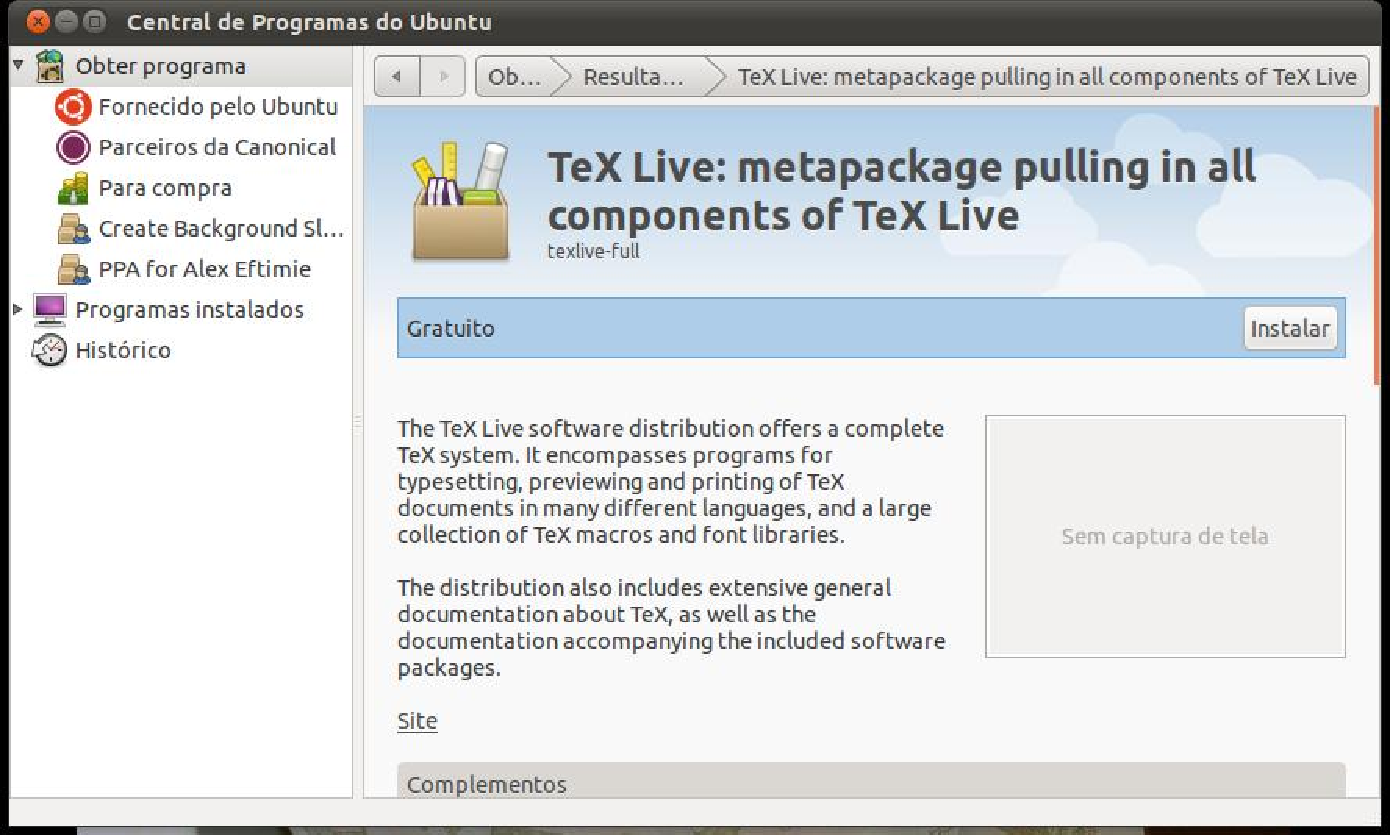
\includegraphics[width=\textwidth,height=.8\textheight,keepaspectratio]{ubuntu}

\end{frame}

%% \begin{frame}{Instalando o \TeX{} Live no Ubuntu-Linux}
%% \begin{itemize}
%% \item O Ubuntu segue as regras do Projeto Debian; Por isso, a instalação da versão \TeX\ Live/Debian é necessária para resolver as dependências  de outros programas Debian, mas esta versão instalada no Ubuntu não é atualizada na mesma velocidade que a produzida para o TUG (\TeX\ Users Group).
%% \item Ambas as instalações podem conviver no mesmo computador. Leia o documento (em italiano):\\
%% {\small\url{http://profs.sci.univr.it/~gregorio/texlive-ubuntu.pdf}}
%% \item Na instalação deve-se assegurar que a data da versão de \TeX\ Live seja sempre a mais recente, e essa é a versão que deve ser usada na preparação de documentos.
%% \end{itemize}
%% \end{frame}

\begin{frame}{Instalando o \TeX{} Live no Ubuntu-Linux}
\begin{block}{Console}
 Usando o apt-get:\\
 apt-get install texlive-full
\end{block}

\begin{block}{Arquivos e mirrors internacionais}
\begin{itemize}
\item O programa de instalação é:
\url{http://mirror.ctan.org/systems/texlive/tlnet/install-tl-unx.tar.gz}

\item Existem muitos mirrors internacionais; veja:
\url{http://ctan.org/mirrors}

\item A instalação de um mirror é preferível já que, geralmente, é mais rápida.
\end{itemize}
\end{block}
\end{frame}

\begin{frame}{\TeX\ Live para MacOS}
\begin{itemize}
\item As máquinas MacOS precisam de uma versão particular do \TeX~Live que chama-se \prog{Mac\TeX}.
\item Veja: \url{http://www.tug.org/mactex/}
\item As instruções são mais simples que em outros sistemas e a instalação é mais rápida.
\end{itemize}
\end{frame}

\begin{frame}{Instalando MiK\TeX\ no Windows}
MiK\TeX\ oferece duas instalações:
\begin{itemize}
\item Instalação básica, que permite instalar os pacotes que faltam, 
quando necessário;
\item Instalação completa (preferível).
\end{itemize}

\end{frame}

\begin{frame}{Instalação da versão MiK\TeX\ básica}
\centering
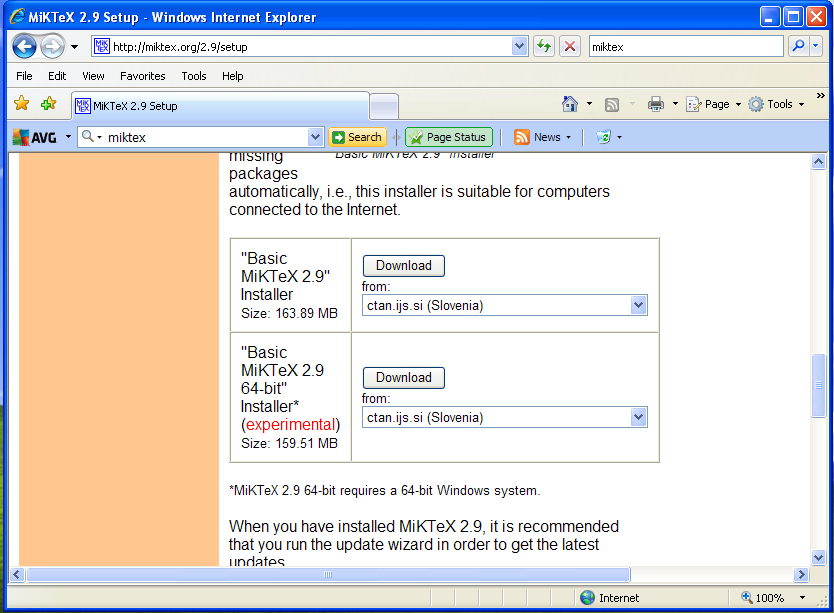
\includegraphics[width=\textwidth,height=\textheight,keepaspectratio]{MiKTeX-Basic}
\end{frame}

\begin{frame}{Instalação da versão MiK\TeX\ completa}
\centering
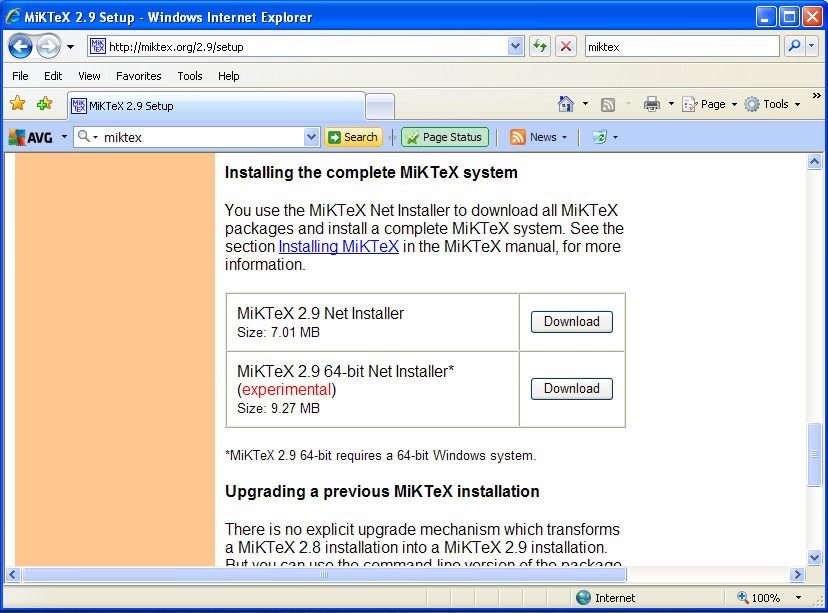
\includegraphics[width=\textwidth,height=\textheight,keepaspectratio]{MiKTeX-Complete}
\end{frame}

%\section{Aula 1}
%% AULA 1
%\section{Aula 1}

\begin{frame}{O que é o \TeX?}
\begin{itemize}
\item \prog{\TeX} é um programa criado por Donald E.~Knuth, usado para desenvolvimento de documentos;
\item Formatador de documentos (como troff e groff -- programas hoje obsoletos);
\end{itemize}
\end{frame}

\begin{frame}{O que faz o \TeX?}
\begin{itemize}
\item Permite desenvolver documentos complexos, incluindo facilidades
  para:
  \begin{itemize}
\item Gerar sumário, index, lista de figuras, lista de 
  tabelas e referências bibliográficas;
\item Importar e tratar imagens de vários formatos  (escalando, rotacionando, convertendo, etc.);
\item Desenvolver gráficos diagramáticos;
\item Representar partituras musicais, partidas de xadrez, fórmulas químicas etc.
\end{itemize}
\end{itemize}

\begin{block}{O poder do \TeX}
O poder do \TeX\ reside em sua habilidade de tratar textos técnicos complicados e exibir fórmulas matemáticas.
\end{block}
\end{frame}

\begin{frame}{Vantagens}
\begin{itemize}
\item Qualidade tipográfica superior (fontes e distribuição do texto
  na página);
\item Compatibilidade (Donald Knuth ``congelou'' o
  programa \TeX);
\item Estabilidade e ausência de falhas (uso prolongado \newline do mesmo programa virtualmente
  eliminou todos os erros);
\item Padrão adotado pela \emph{American Mathematical \newline Society} para
  comunicação entre matemáticos.
\end{itemize}
\end{frame}

\begin{frame}{Formatos usados por \TeX}
\begin{itemize}
\item Os formatos usados por \TeX\ permitem sua livre distribuição (formatos abertos -- TEX, DVI e PDF);
\item Converte para outros formatos (PS, HTML e XML);
\item Existe completa compatibilidade dos documentos.
\end{itemize}
\end{frame}

\begin{frame}{Outras características de \TeX}
\begin{itemize}
\item \TeX\ é multiplataforma (existe para virtualmente qualquer máquina e sistema operacional);
\item \TeX\ enfatiza o \emph{projeto lógico de documentos};
\item \TeX\ é modular;
\item Os recursos do \TeX{} podem ser extendidos pela adição de macros.
\end{itemize}
\end{frame}


\begin{frame}{O que é \LaTeX?}
\begin{itemize}
\item \LaTeX\ é um conjunto padrão de macros para \TeX\ que permite
  um aumento da produtividade no uso do programa;
\item Mais macros podem ser incluidas por meio de pacotes (por exemplo: \Xy-pic, MusiX\TeX, CircuiTikz, etc.);
\item Programas externos, desenvolvidos por programadores e usuários
  de \TeX, extenderam as funcionalidades (por exemplo: BiB\TeX,
  makeindex, etc.).
\end{itemize}
\end{frame}

\begin{frame}{Abordagens para o projeto de documentos}
\begin{itemize}
\item Projeto visual $\times$ projeto lógico de documentos:
\begin{itemize}
\item Projeto visual enfatiza o estético e envolve grande esforço de formatação;
\item Projeto lógico enfatiza a estrutura e economiza tempo pois a formatação é consequência da estrutura;
\item Projeto lógico provoca uma reflexão sobre o texto que tem consequências benéficas até sobre o conteúdo sendo desenvolvido;
\end{itemize}
\end{itemize}
\end{frame}

\begin{frame}{Comparação entre processador de textos e \TeX}
Fórmula obtida usando-se um processador de textos típico:
\begin{center}
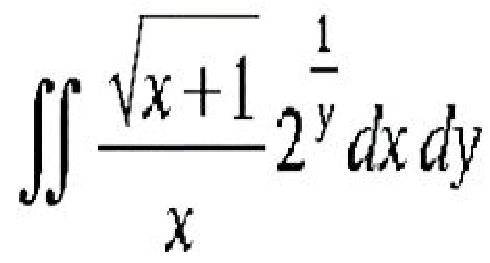
\includegraphics[width=0.5\textwidth]{img/integral.pdf}
\end{center}

Fórmula obtida usando-se \TeX:
\[\int\!\!\!\int\frac{\sqrt{x+1}}{x}2^{\frac{1}{y}}\mathrm{d}x\,\mathrm{d}y\]
\end{frame}

\begin{frame}{Projeto visual $\times$ lógico}
\begin{description}
	\item [Projeto visual] baseado em menus e botões  (o usuário ``desenha'' a fórmula/texto);
	\item [Projeto lógico] baseado em comandos:
\end{description}
	
	\begin{LaTeXcode}[Comandos]
	\string\[\LCmd{int}\string\!\string\!\string\!\LCmd{int}
	\LCmdArg{frac}{\LCmdArg{sqrt}{x+1}}\Larg{x}2\string^\{
	 \LCmdArg{frac}{1}\Larg{y}\}\n
	 \LCmdArg{mathrm}{d}x\string\,\LCmdArg{mathrm}{d}y\string\]
	\end{LaTeXcode}

Produz:
	\begin{LaTeXoutput}[]
	\[\int\!\!\!\int\frac{\sqrt{x+1}}{x}2^{\frac{1}{y}}\mathrm{d}x\,\mathrm{d}y\]
    \end{LaTeXoutput}
\end{frame}

\begin{frame}{Observações}
\begin{itemize}
\item \texttt{\string\[ } e \texttt{\string\]} -- entra e sai do modo matemático;
\item \LCmd{int} -- integral;
\item \texttt{\string\!} -- espaço negativo (para obter o espaçamento correto na integral dupla) -- poderia ter sido usado o comando \LCmd{iint};
\item \LCmdArg{frac}{\ldots}\Larg{\ldots} -- fração;
\item \LCmdArg{sqrt}{\ldots} -- raiz quadrada;
\item \texttt{\string^} -- expoente;
\item \texttt{\string\,} -- espaço pequeno;
\item \LCmdArg{mathrm}{\ldots} -- fonte romano do modo matemático.
\end{itemize}
\end{frame}

\begin{frame}{Projeto lógico}
\begin{itemize}
	\item No projecto lógico, o aspecto estético depende do contexto/estrutura (por 
	exemplo, se a fórmula está dentro de um parágrafo ou destacada do parágrafo). 
	Exemplo:
	\begin{itemize}
		\item O somatório $\sum_{i=0}^\infty a_i/2$ resulta em \dots		
		\item O somatório \[\sum_{i=0}^\infty \frac{a_i}{2}\] resulta em \dots
	\end{itemize}
\end{itemize}
\end{frame}

\begin{frame}{Autor, designer e tipógrafo}
\begin{itemize}
\item Tipografia tradicional: autor $\longrightarrow$ designer $\longrightarrow$ tipógrafo;
\item Designer: responsável pelo layout do documento (escolha dos fontes, número de colunas, margens, etc.). Trabalha baseado em sua percepção do que o autor deseja e em seu conhecimento das regras da tipografia (que privilegiam a facilidade de leitura e não a beleza estética);
\item Tipógrafo: interpreta as anotações geradas pelo designer e produz a matriz para impressão do documento.
\end{itemize}
\end{frame}

\begin{frame}{Tipografia}
\centering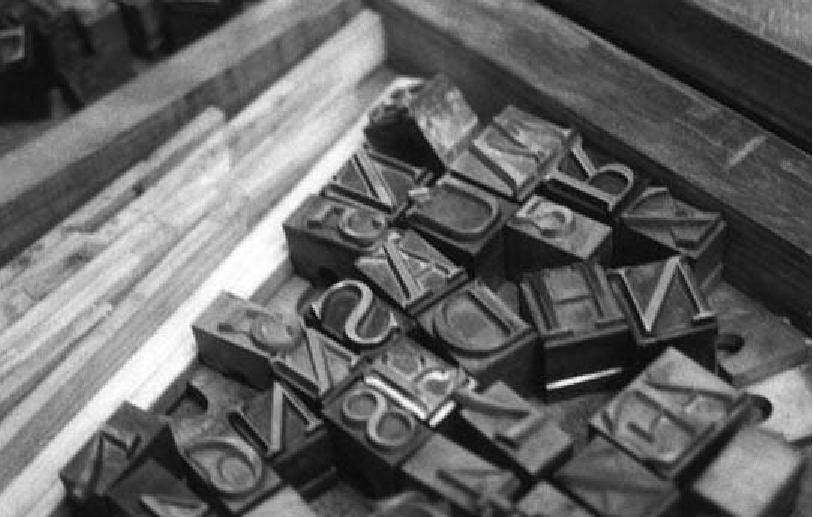
\includegraphics[width=0.85\textwidth]{img/tipografia.pdf}
\end{frame}

\begin{frame}{Funcionamento do \TeX{} e \LaTeX}
\begin{itemize}
\item \LaTeX\ interpreta o papel do designer;
\item \TeX\ interpreta o papel do tipógrafo.
\end{itemize}
\end{frame}

\begin{frame}{\TeX\ e \texttt{pdftex} como um compilador}
\begin{itemize}
\item O programa \TeX\ é um compilador que lê um arquivo de entrada (.TEX) e produz um arquivo de saída (.DVI ou .PDF);
\item O arquivo .TEX é um arquivo ASCII que contém o texto acrescido de comandos ou macros \TeX\ e \LaTeX;
\item O arquivo .DVI usa um formato independente de dispositivo e que pode ser impresso, visualizado ou convertido para outros formatos;
\item Nas versões modernas de \TeX\ o programa de compilação é o \texttt{pdftex}, que pode produzir tanto um arquivo .DVI quanto um arquivo .PDF (Portable Document Format), o qual apresenta vantagens se comparado com o formato DVI -- tornando o formato DVI um pouco obsoleto.
\end{itemize}
\end{frame}

\begin{frame}{Os comandos do \LaTeX}
\begin{itemize}
	\item Os comandos são necessários para que \LaTeX\ possa formatar o texto 
	(\LaTeX\ não é tão inteligente como um designer/tipógrafo humano);
	%
	\item Os comandos \TeX\ normalmente são antecedidos de 
	``\texttt{\textbackslash}'' (por exemplo, para obter \LaTeX\ deve-se digitar 
	\LCmd{LaTeX} e para obter ``\textbackslash'' 	deve-se digitar 
	\texttt{\$}\LCmd{backslash}\texttt{\$} ou \LCmd{textbackslash});
	%
	\item A linguagem \TeX\ segue as regras/ideias de linguagens de programação 
	(declarações e corpo do programa; ligação de bibliotecas; regras de escopo; 
	etc.);
\end{itemize}
	
    \begin{block}{Observação}
    Maiúsculas $\neq$ minúsculas.
    \end{block}
\end{frame}

\begin{frame}{Como funciona o processo de compilação}
\begin{itemize}
\item  \LaTeX{} funciona como um compilador de uma passagem, gerando ao final do processo de compilação um arquivo .AUX que será lido no início da próxima execução do programa;
\item Por isto, frequentemente é necessário compilar mais de uma vez o fonte para resolver todas as pendências;
\item Ao final da execução de \LaTeX, é gerado também um arquivo .LOG contendo informações sobre a compilação.
\end{itemize}
\end{frame}

\begin{frame}{Editando o documento \TeX}
Existem diversos editores ASCII que se adaptam bem para o uso com \TeX: \prog{Emacs}, \prog{TeXmaker}, \prog{\TeX{works}}, \prog{TeXstudio}, \prog{TeXShop}, \prog{WinEdt}, \prog{\TeX{}nicCenter}, etc.
\end{frame}

\begin{frame}{Emacs}
\begin{itemize}
\item Editor disponível para Linux, Windows e MacOS, entre outras plataformas;
\item Veja: \url{http://www.gnu.org/software/emacs/}

\vspace{0.3cm}

\centering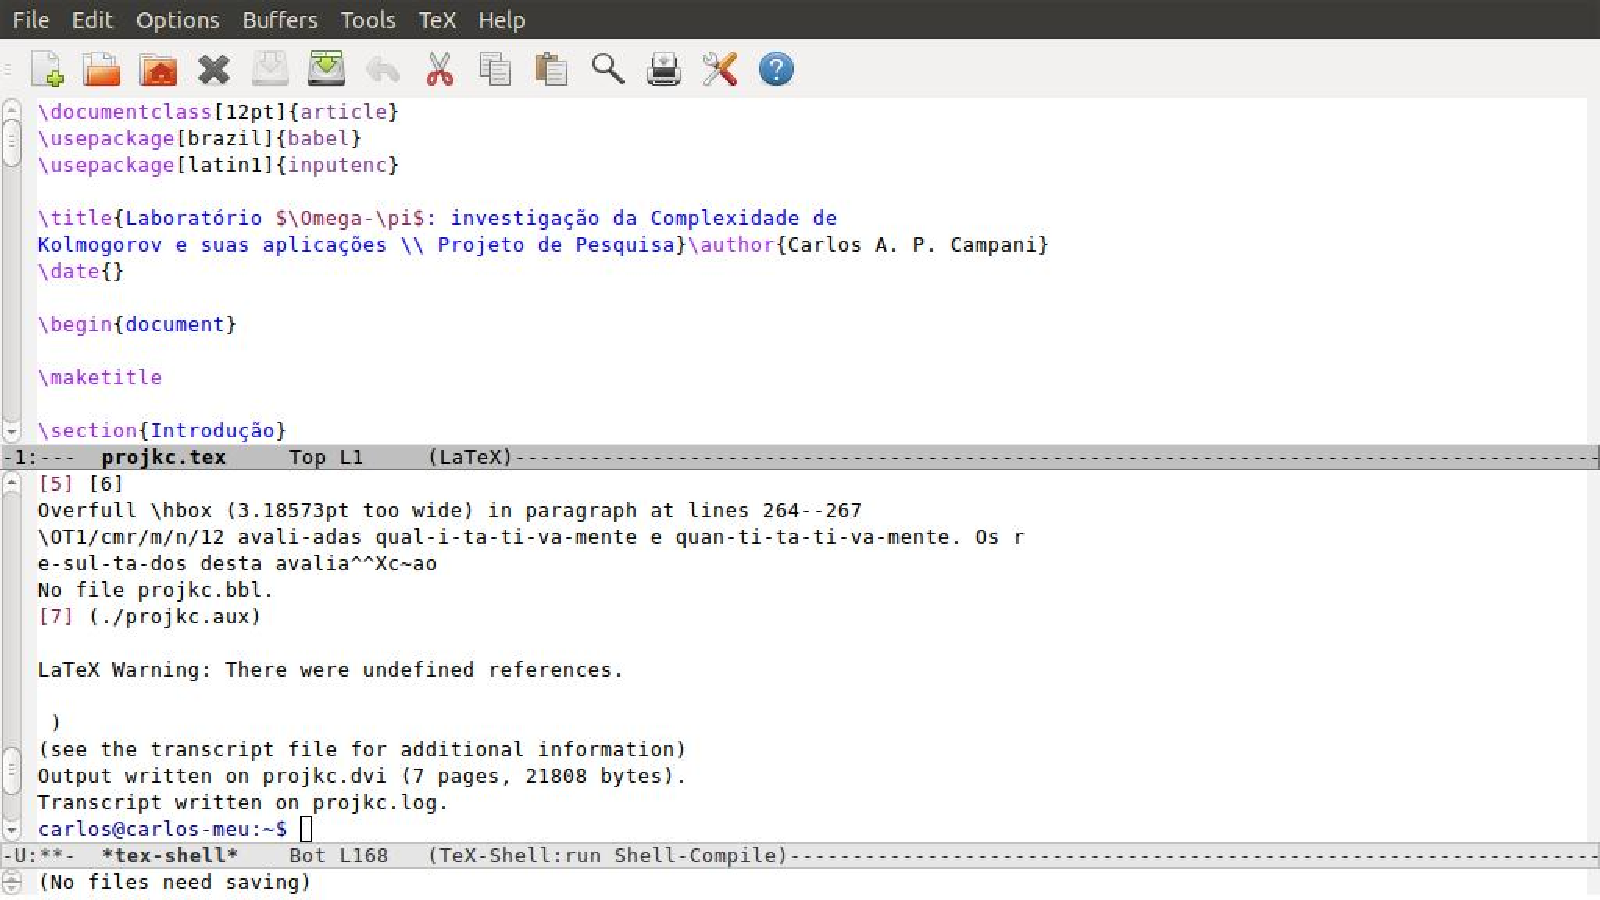
\includegraphics[width=0.85\textwidth]{img/emacs.pdf}
\end{itemize}
\end{frame}

\begin{frame}{TeXmaker}
\begin{itemize}
\item Disponível para Linux, Windows e MacOS
\item Veja: \url{http://www.xm1math.net/texmaker/}

\vspace{0.5cm}

\centering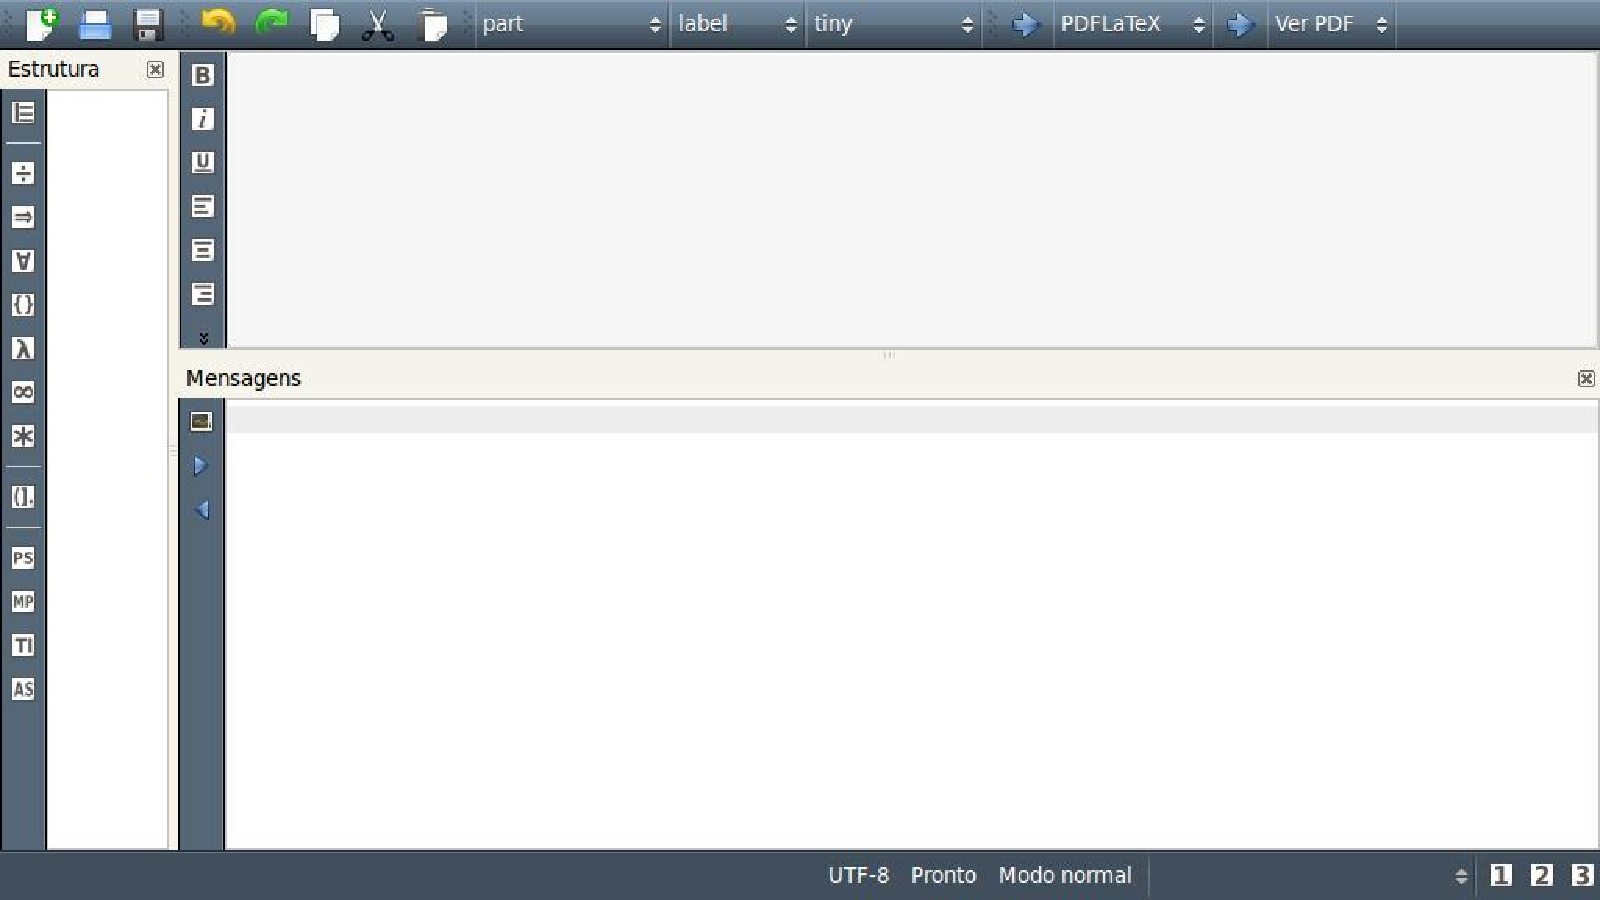
\includegraphics[width=0.85\textwidth]{img/texmaker.pdf}
\end{itemize}
\end{frame}

\begin{frame}{\TeX{works}}
\begin{itemize}
\item Disponível para Linux, Windows e MacOS
\item Veja: \url{http://www.tug.org/texworks/}

\vspace{0.25cm}

\centering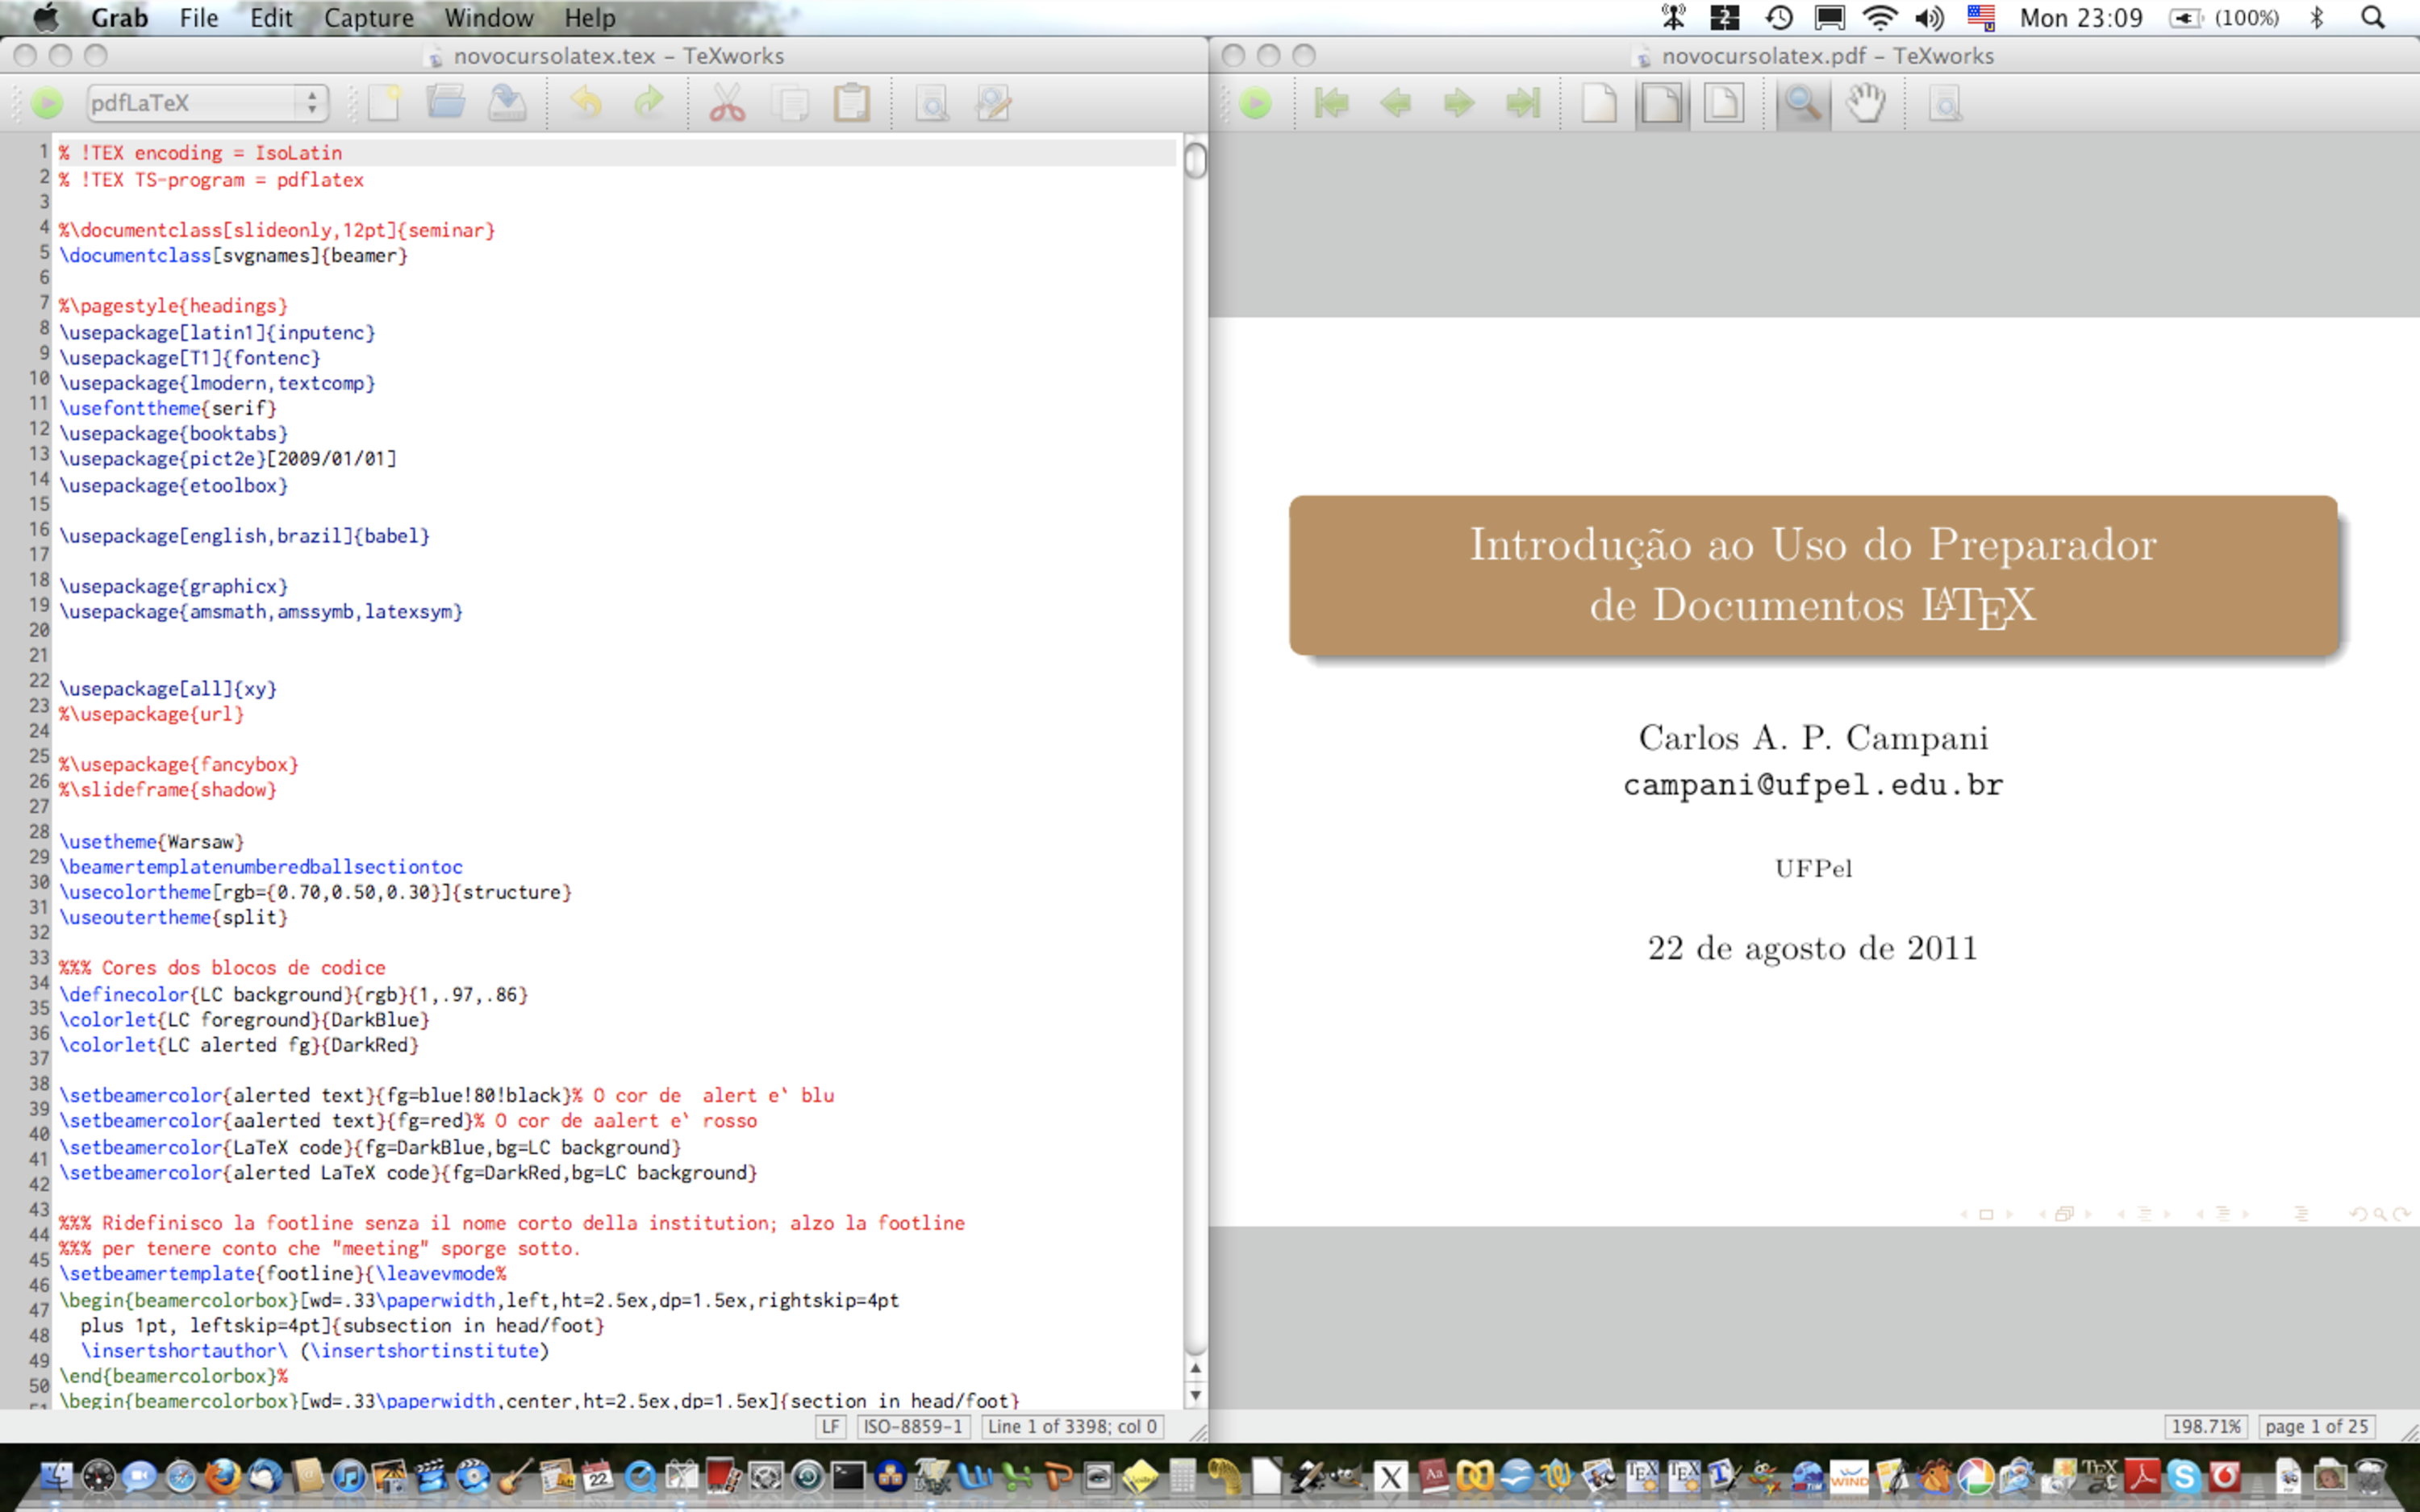
\includegraphics[width=0.80\textwidth]{img/TeXworksPDF.pdf}
\end{itemize}
\end{frame}


\begin{frame}{TeXShop}
\begin{itemize}
\item Disponível somente para MacOS
\item Instalado com Mac\TeX.
\end{itemize}

\centering
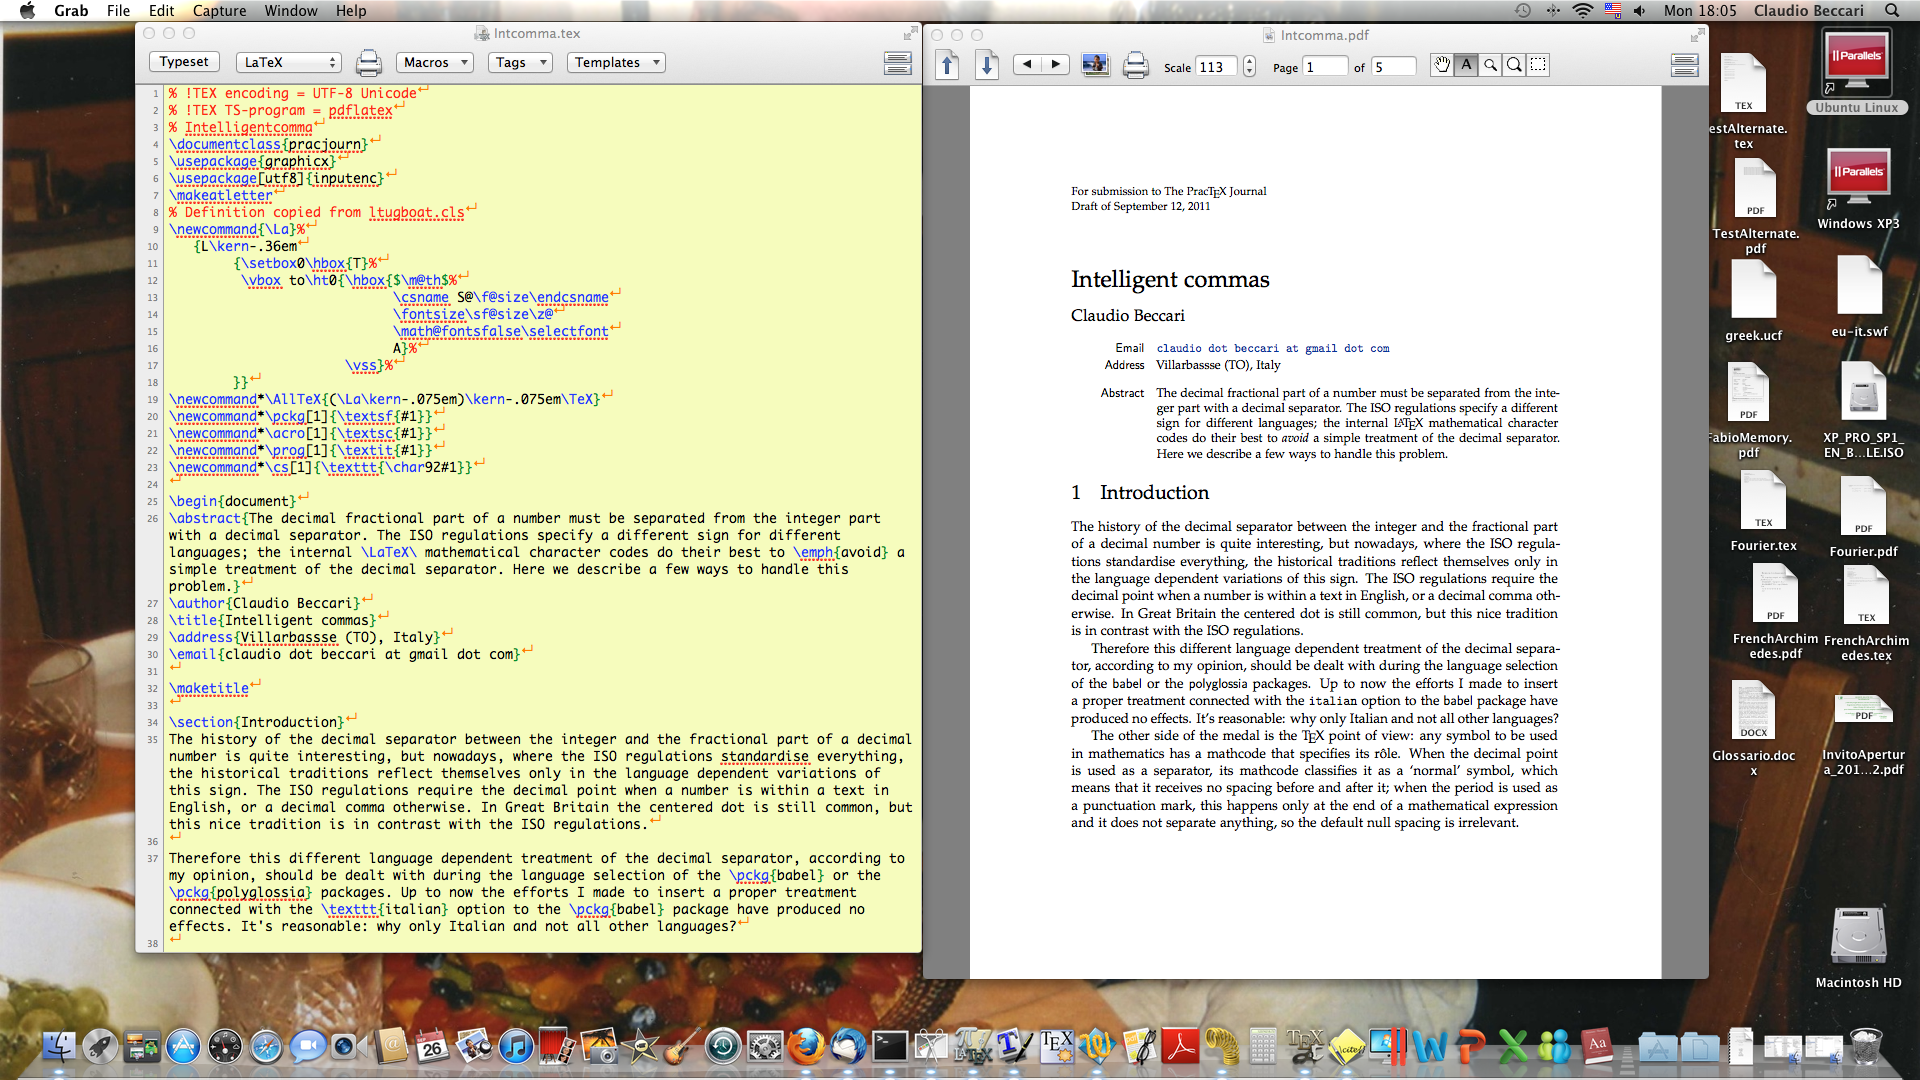
\includegraphics[width=\textwidth,height=.7\textheight,keepaspectratio]{img/TeXShopPNG.png}
\end{frame}

\begin{frame}{WinEdt}
\begin{itemize}
\item Programa shareware;
\item Disponível somente para Windows
\item Veja: \url{http://www.winedt.com/}

\centering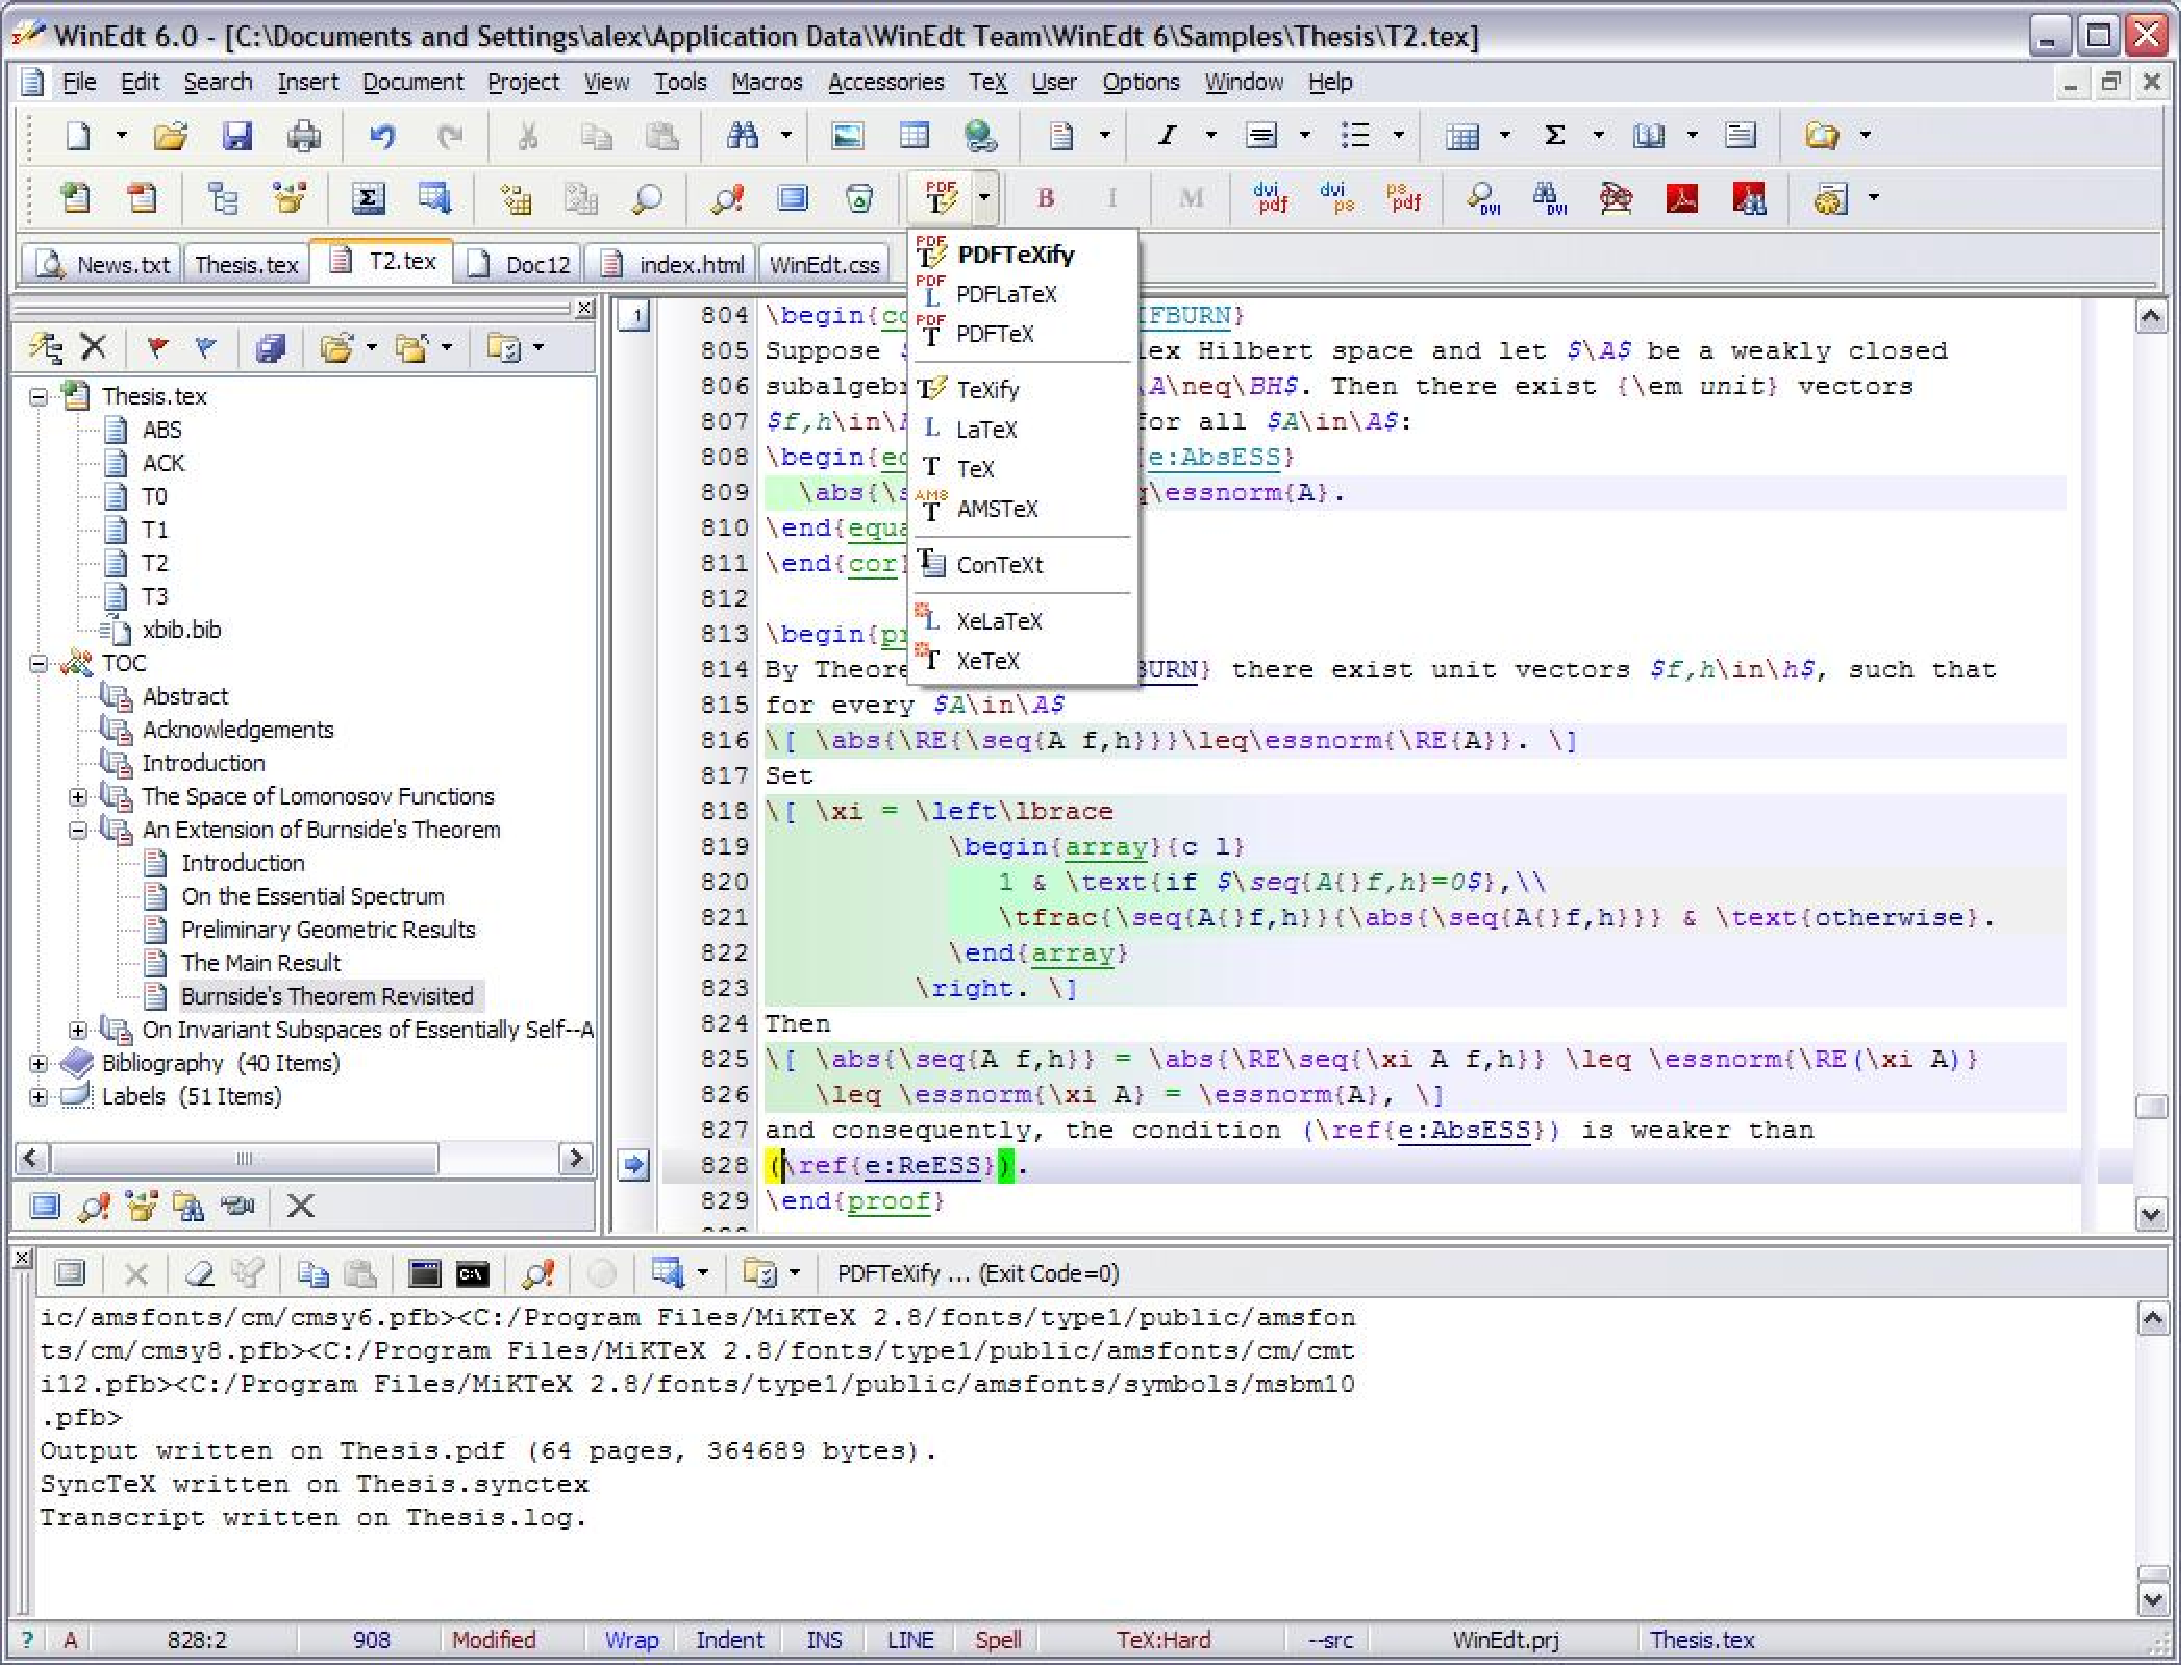
\includegraphics[width=0.65\textwidth]{img/WinEdt.pdf}
\end{itemize}
\end{frame}

\begin{frame}{\TeX{}nicCenter}
\begin{itemize}
\item Disponível somente para Windows
\item Veja: \url{http://www.texniccenter.org/}

\vspace{0.5cm}

\centering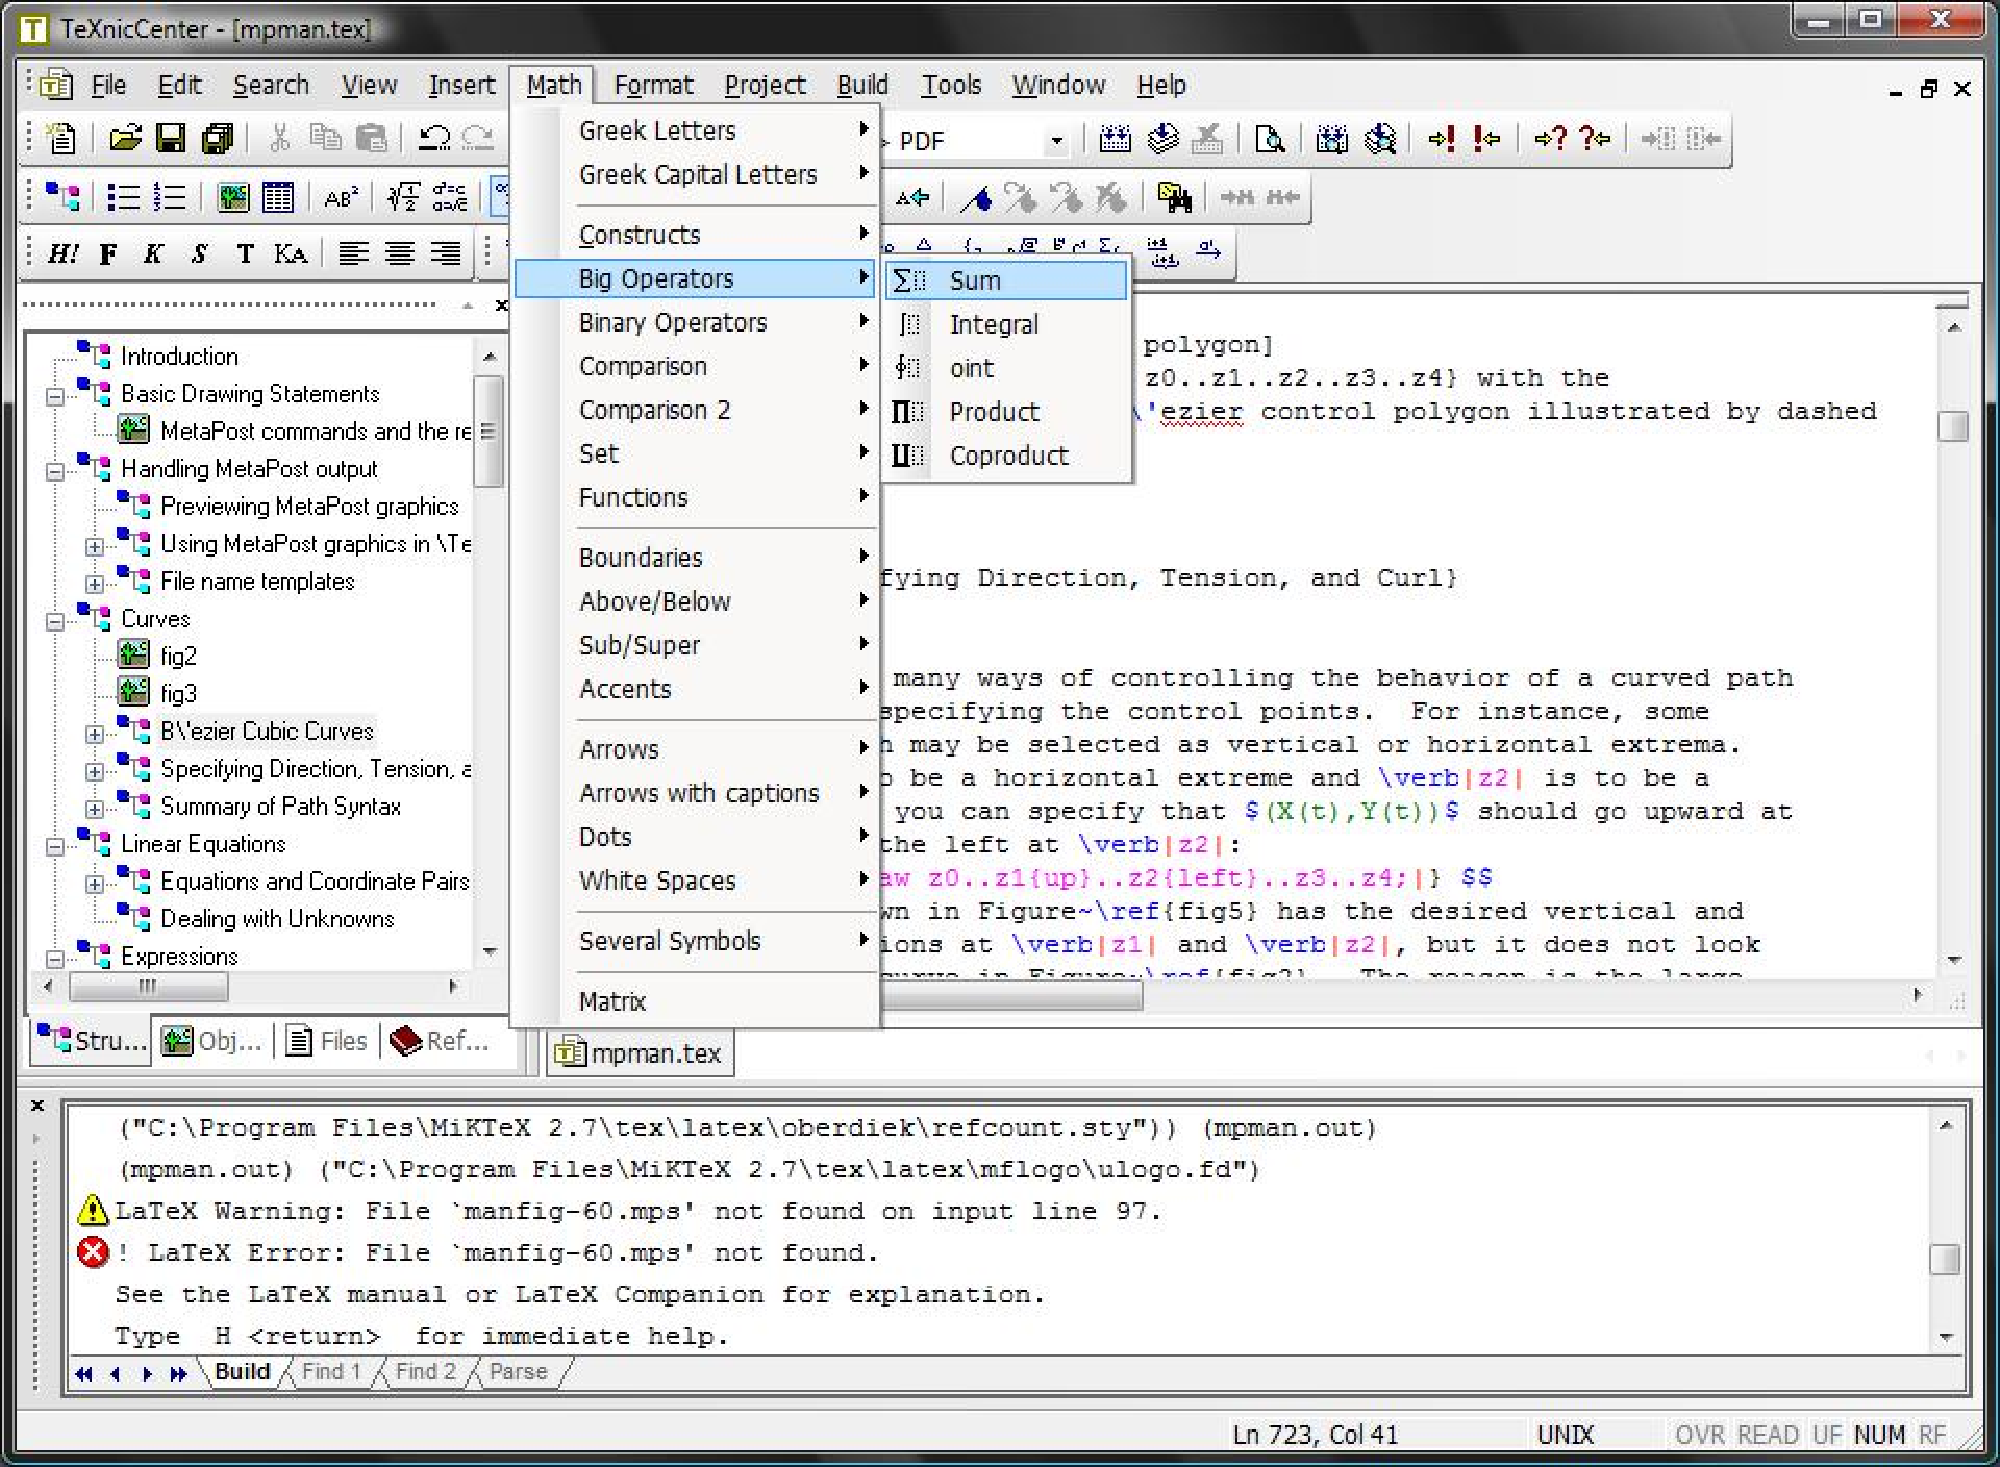
\includegraphics[width=0.70\textwidth]{img/texniccenter.pdf}
\end{itemize}
\end{frame}

\begin{frame}{ShareLaTex}
Editor On-Line: \url{http://sharelatex.com}
\begin{center}
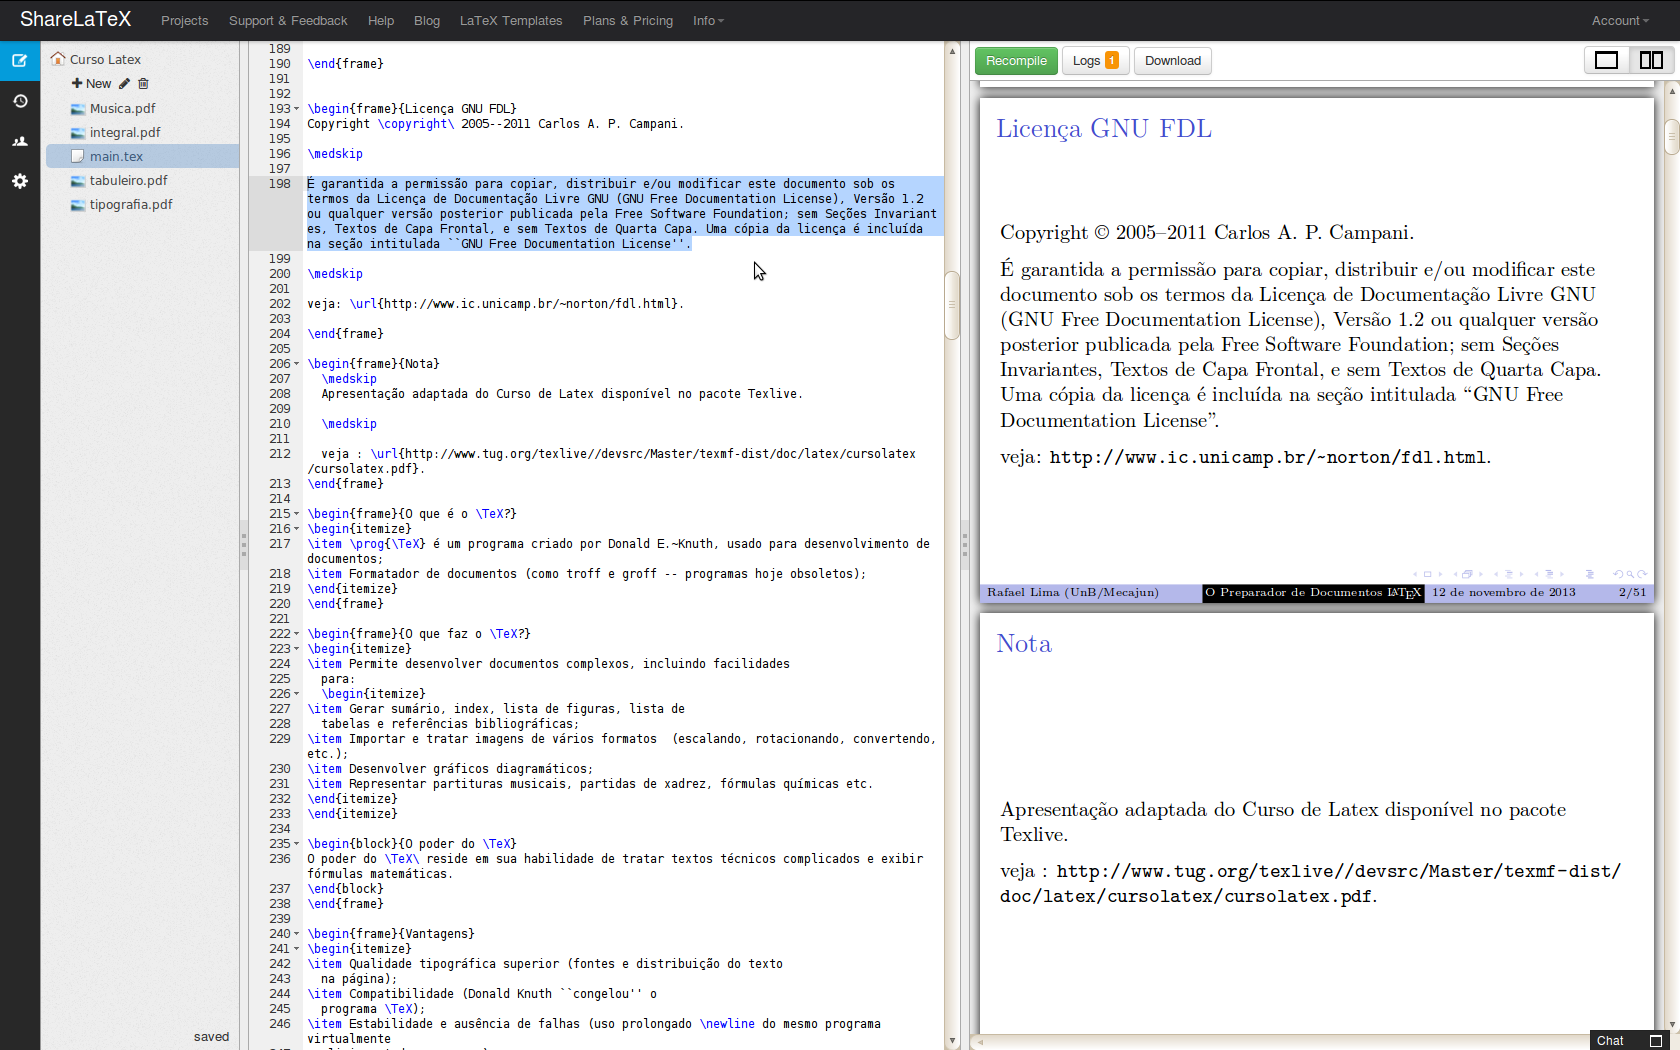
\includegraphics[width=0.85\textwidth]{img/sharelatex.png}
\end{center}
\end{frame}

\begin{frame}{LyX}
Editor WYSWG\footnote{WYSWG - What You See What You Get} para LaTeX % /TODO Explicar o termo WYSWG
\begin{center}
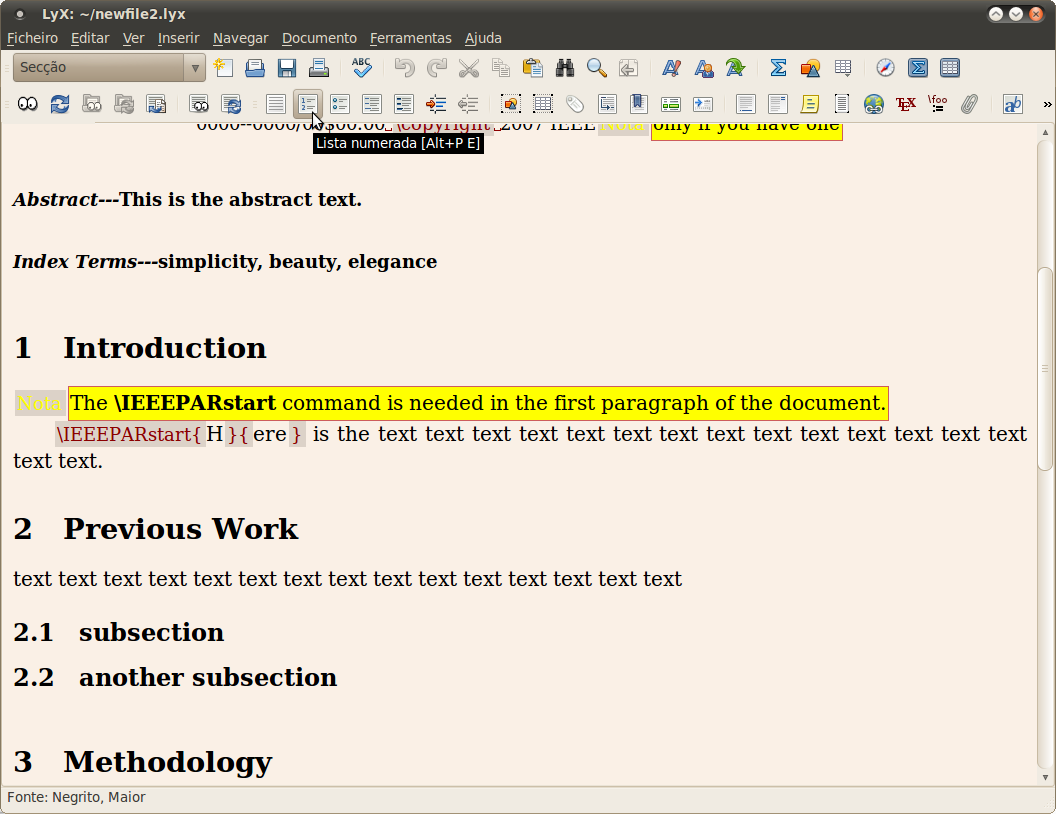
\includegraphics[width=0.70\textwidth]{img/LyX.png}
\end{center}
\end{frame}

\begin{frame}[fragile] % /TODO Verificar este slide
\frametitle{Compilando, visualizando e imprimindo}
\begin{itemize}
\item Compilação: Abrir o Terminal do Linux e usar o comando \verb+$ pdflatex teste.tex+ (para compilar, por exemplo, o arquivo \verb+teste.tex+) ou usar o menu \emph{TeX/TeX File} no \prog{Emacs}. No \prog{\TeX{works}} clicar no botão verde;
\item Visualização: \verb+$ xdg-open teste.pdf+ (o arquivo é recarregado automaticamente a cada modificação). Em alguns programas o resultado em .PDF aparece direitamente numa segunda janela;
\item Convertendo para html: \verb+$ latex2html teste.tex+;
\item Imprimindo: \verb+$ dvips teste.dvi+ ou \verb+$ lpr teste.ps+ no Terminal do Linux. Para imprimir no \prog{\TeX{Shop}} use \emph{File/Print}
\end{itemize}
\end{frame}

\begin{frame}{Estrutura e comandos \LaTeX}
\begin{LaTeXcode}[Estrutura geral]
\LCmdOptArg{documentclass}{opcionais}{classe}\n
declarações\n
\LCmdArg{begin}{document}\n
documento\n
\LCmdArg{end}{document}
\end{LaTeXcode}

\medskip

\begin{LaTeXcode}[Para trabalhar com arquivos grandes]
\LCmdArg{include}{nomearquivo}
\% inclui comandos de um arquivo\n \% gera nova página antes\nn
\LCmdArg{input}{nomearquivo} 
\% inclui comandos de um arquivo\n \% não gera nova página
\end{LaTeXcode}
\end{frame}

\begin{frame}{Estrutura dos comandos}
\begin{itemize}
\item Comandos \LaTeX{} são normalmente precedidos por \texttt{\textbackslash} e seguidos de parâmetros opcionais (delimitados por ``\texttt{[}`` e ``\texttt{]}'') e/ou parâmetros obrigatórios (delimitados por ``\texttt{\lb}'' e ``\texttt{\rb}'');
\begin{LaTeXcode}[Exemplos]
\LCmd{TeX}\n
\LCmd{LaTeX}\n
\LCmdArg{documentclass}{book}\n
\LCmdOptArg{documentclass}{12pt}{article}\n
\LCmdArg{begin}{document}
\end{LaTeXcode}

\bigskip

\item Uma excessão a esta regra é ``\texttt{\$}'' que delimita o ambiente matemático. Exemplo: \texttt{\$3+2\LCmdArg{sqrt}{2}\$}, que produz $3+2\sqrt{2}$.
\end{itemize}
\end{frame}

\begin{frame}{Espaços}
\begin{itemize}
\item Diversos espaços em branco, tabulações e novas linhas são desprezados (são considerados como um ``espaço branco simples'');
\item Os espaços adicionais são consumidos.
\end{itemize}
\end{frame}

\begin{frame}{Espaços após um comando \TeX}
Espaços após um comando serão consumidos até encontrar um caracter diferente de branco, resultando que
\begin{LaTeXcode}
\LCmd{TeX} é legal!
\end{LaTeXcode}
Produz:

\begin{LaTeXoutput}
\TeX é legal!
\end{LaTeXoutput}

Para evitar isto, use \texttt{\textbackslash\textvisiblespace}\footnote{O símbolo \texttt{\textvisiblespace}  serve para representar o espaço no texto fonte.} ou \texttt{\{\}}, que interrompe o consumo de espaços em branco, ou \texttt{\textasciitilde} (espaço em branco indivisível):
\begin{LaTeXcode}
\LCmd{TeX}\textbackslash\textvisiblespace é legal!\n
ou\n
\LCmd{TeX}\{\}\textvisiblespace é legal!\n
ou\n
\LCmd{TeX}\textasciitilde é legal!
\end{LaTeXcode}
\end{frame}

\begin{frame}{Delimitação de parágrafos}
Uma ou mais linhas em branco delimita os parágrafos:

\begin{LaTeXcode}[Exemplo]
Este é o\textvisiblespace\textvisiblespace\textvisiblespace\textvisiblespace primeiro \n parágrafo.\n

E este é o segundo!
\end{LaTeXcode}

Produz:
\begin{LaTeXoutput}
Este é o         primeiro
parágrafo.

E este é o segundo!
\end{LaTeXoutput}
\end{frame}

\begin{frame}{Comentários no arquivo fonte}
Comentários em \TeX\ são obtidos usando-se \texttt{\%}

Exemplo:
\begin{LaTeXcode}[Arquivo fonte com comentários]
Este é um exemplo\n
\% comentários são considerados\n
\% espaços em branco\n
de uso de comentários. \% fim do exemplo
\end{LaTeXcode}

Produz:
\begin{LaTeXoutput}
Este é um exemplo
% comentários são considerados
% espaços em branco
de uso de comentários. % fim do exemplo
\end{LaTeXoutput}
\end{frame}

\begin{frame}{Classes disponíveis}
\begin{itemize}
\item Principais classes disponíveis:
\begin{description}
\item [\Lcls{article}] Artigos curtos;
\item [\Lcls{report}] Artigos mais longos, monografias, relatórios;
\item [\Lcls{book}] Livros;
\end{description}

\medskip

\item Principais opções: 

\medskip

\begin{itemize}
\item \Lopt{11pt} -- fonte de 11 pontos;
\item \Lopt{12pt} -- fonte de 12 pontos;
\item \Lopt{twoside} -- imprime em ambos os lados da página;
\item \Lopt{twocolumn} -- produz saída em duas colunas.
\end{itemize}

\medskip

\item Lembre-se: \LCmdOptArg{documentclass}{opções}{classe}
\end{itemize}
\end{frame}

\begin{frame}{Estilos de página}
\begin{LaTeXcode}
\LCmdArg{pagestyle}{estilo}\n
ou\n
\LCmdArg{thispagestyle}{estilo}
\end{LaTeXcode}

Estilos disponíveis:

\begin{description}
\item [plain] número de página centralizado no rodapé;
\item [headings] capítulo corrente e número de página no cabeçalho;
\item [empty] cabeçalho e rodapé vazios;
\end{description}
\end{frame}

\begin{frame}{Ambientes}
O \LaTeX{} trabalha com \emph{ambientes}; o escopo de um ambiente é
definido pelos comandos \LCmdArg{begin}{\dots} e
\LCmdArg{end}{\dots}. Exemplos:

\begin{LaTeXcode}
\LCmdArg{begin}{document}
...
\LCmdArg{end}{document}
\end{LaTeXcode}
e
\begin{LaTeXcode}
\LCmdArg{begin}{center}
...
\LCmdArg{end}{center}
\end{LaTeXcode}
\end{frame}

\begin{frame}{Exemplo de um arquivo .TEX simples}
\begin{LaTeXcode}[Exemplo de arquivo .TEX]
\LCmdOptArg{documentclass}{12pt}{article}\n
\LCmdArg{begin}{document}\n
Oi, mundo!\n

Eu sou \LCmd{LaTeX}!\n
\LCmdArg{end}{document}
\end{LaTeXcode}
que produz na saída:

\begin{LaTeXoutput}
Oi, mundo!

Eu sou \LaTeX!
\end{LaTeXoutput}
\end{frame}

\begin{frame}{Usando pacotes}

\begin{itemize}
\item Amplia as funcionalidades do \LaTeX;
\item Modularidade;
\item \LOA{usepackage}[opções]{pacote};
\end{itemize}
\end{frame}

\begin{frame}{Usando pacotes}
\begin{LaTeXcode}[Exemplo]
\LCmdArg{documentclass}{article}\n
\LOA usepackage[brazilian]{babel}\n
\LOA usepackage[latin1]{inputenc}\n
\LOA usepackage[T1]{fontenc}\n
\LCmdArg{usepackage}{lmodern}\n
\LCmdArg{usepackage}{graphicx}\n
\LCmdArg{usepackage}{amsmath,amssymb}\n
\LCmdArg{usepackage}{indentfirst}\n
\LCmdArg{usepackage}{url}\n
\LCmdArg{begin}{document}\n
\dots\n
\LCmdArg{end}{document}
\end{LaTeXcode}
\end{frame}

\begin{frame}{Usando pacotes}\fontsize{10}{11}\selectfont
\begin{lista}
\item [babel] determina a língua usada no texto (\Lopt{brazilian}  é o português com as variantes brasileiras);
\item [inputenc] determina a codificação usada (use  \Lopt{latin1} no Linux, \Lopt{ansinew} no Windows e \Lopt{utf8} para a codificação universal UNICODE);
\item[fontenc] determina a codificação dos fontes usados na saída; para o português é importante usar a codificação \Lopt{T1};
\item[lmodern] escolhe um fonte vetorial com a codificação \Lopt{T1} (melhora a qualidade dos fontes no PDF);
\item [graphicx] permite incorporar imagens no texto (formatos PDF, JPG, PNG, MPS e EPS);
\item [amsmath e amssymb] fontes e símbolos  matemáticos adicionais da AMS;
\item [indentfirst] indentação em início do primeiro parágrafo de seção;
\item [url] permite colocar urls no texto usando o comando \LCmdArg{url}{http://\dots}.
\end{lista}

\end{frame}

\begin{frame}{Definindo divisões do texto}
\LaTeX\ gera automaticamente a numeração das seções, existindo os 
seguintes comandos para a sua numeração:

\begin{LaTeXcode}[Comandos de divisão do texto]
\LCmd{part}\n
\LCmd{chapter}\n
\LCmd{section}\n
\LCmd{subsection}\n
\LCmd{subsubsection}\n
\LCmd{paragraph}\n
\LCmd{subparagraph}
\end{LaTeXcode}

A classe \Lcls{article} não permite o comando \LCmd{chapter}.
\end{frame}

\begin{frame}{Divisões do texto}
\begin{LaTeXcode}[Exemplo]
\LCmdArg{documentclass}{article}\n
\LOA usepackage[brazilian]{babel} \LOA usepackage[utf8]{inputenc}\n
\LOA usepackage[T1]{fontenc} \LCmdArg{usepackage}{lmodern}\n
\LCmdArg{begin}{document}\n
\LCmdArg{section}{Introdução}\n
bla, bla, bla\n
\LCmdArg{section}{Usando o \LCmd{LaTeX}}\n
\LCmdArg{subsection}{Uso Básico}\n
bla, bla, bla\n
\LCmdArg{subsection}{Uso Avançado}\n
\LCmdArg{section}{Conclusão}\n
bla, bla, bla\n
\LCmdArg{end}{document}
\end{LaTeXcode}
\end{frame}

\begin{frame}{Símbolos especiais}
Os seguintes sete símbolos especiais podem ser facilmente obtidos 
pelos seguintes comandos:

\begin{center}
\begin{tabular}{r*6c}
\$ &\& &\% &\# &\_ &\{ &\} \\
\LCmd{\$} &\LCmd{\&} &\LCmd{\%} &\LCmd{\#} &\LCmd{\textunderscore} &\LCmd{\lb} &\LCmd{\rb}
\end{tabular}
\end{center}

Esses símbolos são especiais porque são usados em comandos na sintaxe de \LaTeX{} e não podem ser obtidos direitamente.
\end{frame}

\begin{frame}[fragile]
\frametitle{Acentos e cedilha no texto}
\begin{center}\let\tt\ttfamily
\begin{tabular}{*7c}
ò & ó & ô & ö & õ & ç & Ç \\
\LCmdArg{`}{o} &\LCmdArg{'}{o} &\LCmdArg{\textasciicircum}{o} &\LCmdArg{\string"}{o} &\LCmdArg{\textasciitilde}{o} &\LCmdArg{c}{c} &\LCmdArg{c}{C}
\end{tabular}
\end{center}
\end{frame}

\begin{frame}{Conversão automática dos acentos}
O pacote \texttt{inputenc} faz internamente a conversão automática dos acentos e o usuário não tem de preocupar-se com os comandos de acentuação:

\begin{center}
á $\longrightarrow$ \texttt{\LCmd{'}a}
\end{center}

No entanto, se não existirem recursos no teclado de sua máquina para acentuar, você ainda poderá acentuar seu texto usando os comandos.
\end{frame}

\begin{frame}{Especificação das línguas usadas no documento}
\begin{itemize}
\item O pacote babel especifica as línguas usadas no documento (\Lopt{brazilian}, \Lopt{english}, etc.), definindo, entre outras coisas, as regras de hifenação (separação silábica);
\item A última língua especificada entre as opções é a língua geral do documento;
\item Exemplo:
\begin{LaTeXcode}[Especificação das línguas do documento]
\LOA usepackage[italian,english,brazilian]{babel}
\end{LaTeXcode}
e a língua geral do documento é o português do Brasil.
\end{itemize}
\end{frame}

\begin{frame}{Seleção das línguas do documento}
\begin{itemize}
\item O documento pode ser composto somente nas línguas especificadas no pacote \Lsty{babel}; 
\item A distribuição \TeX\ Live possui suporte para quase 50 línguas;
\item Isso implica que o \LaTeX\ muda as palavras como ``Capítulo'', por exemplo, em ``Chapter'', dependendo da língua escolhida.
\item Pode-se compor um trecho de texto em inglês, em um documento em português, com:
\begin{LaTeXcode}[Seleção local da língua]
\LCmdArg{begin}{otherlanguage}\Larg{english}\n
English text\n
\LCmdArg{end}{otherlanguage}
\end{LaTeXcode}
\end{itemize}
\end{frame}

\begin{frame}{Seleção das línguas do documento}
Um pequeno pedaço de texto em inglês, envolto por texto em português,  pode-se compor com:
\begin{LaTeXcode}[Texto estrangeiro em linha]
texto em português \LCmdArg{foreignlanguage}{english}\Larg{English text}
outro texto em português \dots
\end{LaTeXcode}
\end{frame}

\begin{frame}{Hifenação (divisão silábica)}
A hifenação é feita automaticamente por \LaTeX, desde que o pacote babel tenha sido carregado. No caso de ocorrer uma hifenação incorreta, a correção é feita usando-se:
\begin{LaTeXcode}[Hifenação irregular]
\LCmdArg{hyphenation}{PYTHON com-pu-ta-dor} \% (usado na área\n \% de declarações/correção global)\nn
com\LCmd{-}pu\LCmd{-}ta\LCmd{-}ção \% (usado no corpo do texto/local)
\end{LaTeXcode}
\end{frame}

\begin{frame}{Produzindo texto}
\begin{itemize}
\item Aspas: Não use \texttt{\string"\dots\string"}; use \texttt{`{}`\dots'{}'} que produz ``\dots''. 
\item Apóstrofes: \texttt{d'alembertiano} produz d'alembertiano;
\item Hífens:
\begin{center}\let\tt\ttfamily
\begin{tabular}{ll}
\tt madeira-branca & madeira-branca \\
\tt linhas 117-{}-138 & linhas 117--138 \\
\tt verdadeiro-{}-{}-ou falso? & verdadeiro---ou falso? \\
\tt \$-3.2\$ & $-3.2$
\end{tabular}
\end{center}
\end{itemize}
\end{frame}

\begin{frame}{Reticências}
\begin{itemize}
\item Para exprimir uma reticência no texto, usa-se \LCmd{dots};
\item Note a diferença entre \texttt{...} que produz ... e \texttt{\string\dots} que produz \dots;
\item Três pontinhos não são adequados pois são interpretados como três sentenças vazias;
\item Na matemática existem várias reticências; na linha da base, no meio da linha, e vertical e diagonal nas matrizes:
\begin{center}
\begin{tabular}{ll}
\ldots 		& \LCmd{ldots} \\
\vdots 		& \LCmd{vdots} \\
$\ddots$ 	& \texttt{\$\string\ddots\$}\\
$a,\dots,z$	& \texttt{\$a, \string\ldots, z\$} ou \texttt{\$a, \string\dots, z\$} \\
$a+\dots+ z$	& \texttt{\$a+ \string\cdots+ z\$} ou \texttt{\$a+ \string\dots+ z\$} \\
\end{tabular}
\end{center}
\item \LCmd{dots} sempre produz a reticência adequada pelo contexto.
\end{itemize}
\end{frame}

\begin{frame}{Ligaduras}
\begin{itemize}
\item As ligaduras mas frequentes são:

\medskip

 ff fi fl ffi \ldots ao invés de f{}f f{}i f{}l f{}f{}i;
\item Para evitar use-se um grupo vazio: \texttt{f\{\}f} que produz f{}f.
\end{itemize}

 \bigskip

\begin{block}{Usando a lupa}
{\Huge ff fi fl ffi} \ldots ao invés de {\Huge f{}f f{}i f\mbox{}l f{}f{}i}.
\end{block}
\end{frame}

\begin{frame}{Mudando o estilo do texto}
\let\tt\ttfamily

\begin{tabular}{lll}
				& Comando		& Declaração \\
\textbf{Bold} & \tt\string\textbf\{\dots\}	& \tt\{\string\bfseries \dots\} \\
\texttt{Máquina de escrever} & \tt\string\texttt\{\dots\} & \tt\{\string\ttfamily \dots \}\\
\textit{Itálico} & \tt\string\textit\{\dots\}	& \tt\{\string\itshape\dots\} \\
\textsf{Sans serif} & \tt\string\textsf\{\dots\}& \tt\{\string\sffamily\dots\} \\
\textsc{Small Caps}	& \tt\string\textsc\{\dots\}& \tt\{\string\scshape\dots\} \\
Ênfase  & \tt\string\emph\{\dots\} & \tt\{\string\em \dots\}
\end{tabular}

\begin{itemize}
\item Deve-se observar que o ênfase não usa sublinhado\footnote{O sublinhado jamais é usado em tipografia.}, e é obtido com itálico se o texto é normal e normal se o texto é itálico;
\item Os comandos produzem seu efeito somente sobre seu argumento (escopo);
\item Comandos e/ou declarações podem ser acumulados: \\ \texttt{\string\textbf\{\string\itshape\ Itálico negro\}} produz \textbf{\itshape Itálico negro}.
\end{itemize}
\end{frame}

\begin{frame}{Serifas}
\begin{itemize}
\item As serifas são os pequenos traços ou hastes que ocorrem nos prolongamentos das letras;
\item Servem para guiar o olhar ao longo do texto;
\item As serifas na base das letras formam uma linha que serve como referência para o olho ``trafegar'' na linha de texto (como um trem no trilho);
\item Ela aumenta a legibilidade do corpo do texto\footnote{Jamais se usa fonte \emph{sans serif} no corpo do texto.}.

\begin{block}{Comparação}
\centering{\Large\string_\string_\textrm{Com serifa}\string_\string_ \hspace{2cm} \string_\string_\textsf{Sem serifa}\string_\string_}
\end{block}
\end{itemize}
\end{frame}

\begin{frame}{Mudando o tamanho dos fontes}
\let\tt\ttfamily

\begin{center}
\begin{tabular}{ll}
\tiny tiny & \tt\{\string\tiny\ \dots\} \\
\scriptsize scriptsize & \tt\{\string\scriptsize\ \dots\} \\
\footnotesize footnotesize & \tt\{\string\footnotesize\ \dots\} \\
\small small & \tt\{\string\small\ \dots\} \\
\normalsize normalsize &\tt\{\string\normalsize\ \dots\} \\
\large\strut large & \tt\{\string\large\ \dots\} \\
\Large\strut Large & \tt\{\string\Large\ \dots\} \\
\LARGE\strut LARGE & \tt\{\string\LARGE\ \dots\} \\
\huge\strut huge & \tt\{\string\huge\ \dots\} \\
\Huge\strut Huge & \tt\{\string\Huge\ \dots\}
\end{tabular}
\end{center}

\begin{block}{}
Escopo da definição delimitado pelo grupo.
\end{block}
\end{frame}

\begin{frame}{Alinhamento do texto}
Ambientes \emph{center}, \emph{flushleft} e \emph{flushright}:

\begin{center}
\Huge Centrado
\end{center}

\begin{flushleft}
\Huge Esquerda
\end{flushleft}

\begin{flushright}
\Huge Direita
\end{flushright}
\end{frame}

\begin{frame}{Sobre espaçamento}\fontsize{10}{12}\selectfont
\begin{itemize}
\item Para produzir espaço no texto pode-se usar ``\LCmd{\textvisiblespace}'', que representa o espaço simples;
\item Para produzir espaço negativo: \texttt{\string\!};
\item ``\texttt{\textasciitilde}'' produz um espaço que não pode ser dividido em uma quebra de linha; por exemplo: \texttt{fone:\ 51\textasciitilde5551234};
\item \TeX\ assume que sentenças terminam com ``.'', introduzindo um espaço adicional ao final da frase. O comando \LCmd{frenchspacing} desabilita este espaço adicional;
\item Para obter espaço vertical: \LCmdArg{vspace}{espaço} (não permite obter espaço no início de uma página) e \LCmdArg{vspace*}{espaço} (conserva o espaço no início de uma página);
\item \LCmdArg{hspace}{espaço} permite obter espaço horizontal dentro de uma linha;
\item Pode-se usar as dimensões em pontos (pt), polegadas (in), milímetros (mm), centímetros (cm) etc.
\end{itemize}
\end{frame}

\begin{frame}{Quebra de linha, parágrafo e página}


\begin{itemize}
\item Quebra de linha: \texttt{\string\\ } ou \texttt{\string\newline};
\item Quebra de página: \texttt{\string\newpage}.
\end{itemize}

\end{frame}

\begin{frame}{Notas de rodapé}


As notas de rodapé podem ser obtidas colocando-se, no lugar do 
texto onde deve ser referenciada a nota, o comando \LCmdArg{footnote}{Texto da nota}, tendo como argumento o texto da nota. 

\begin{LaTeXcode}[Exemplo]
42\LCmdArg{footnote}{A resposta para a vida o universo e tudo mais}
\end{LaTeXcode}

Produz a saída:
\begin{LaTeXoutput}
42\footnote{A resposta para a vida o universo e tudo mais}
\end{LaTeXoutput}
\end{frame}

\begin{frame}{Produzindo títulos de trabalhos}
\begin{LaTeXcode}[Declarações]
\LCmdArg{title}{Título}\n
\LCmdArg{author}{Autor}\n
\LCmdArg{date}{Data} ou \LCmdArg{date}{}
\end{LaTeXcode}

Observações:
\begin{itemize}
\item \texttt{\string\date\{\}} omite a data do documento;
\item Omitindo-se o comando \texttt{\string\date}, é tomada a data corrente da máquina.
\end{itemize}

\begin{LaTeXcode}[Produzindo]
\LCmd{maketitle}
\end{LaTeXcode}
\end{frame}

\begin{frame}{Exemplo de uso de título de trabalho}
\begin{LaTeXcode}[Estrutura no fonte]
\LCmdArg{documentclass}{book}\n
\LCmdArg{title}{O Guia do Mochileiro das Galáxias}\n
\LCmdArg{author}{Douglas Adams}\n
\LCmdArg{date}{}\n
\LCmdArg{begin}{document}\n
\LCmd{maketitle}\n

O Universo é tão grande que comparado a ele mesmo ele é infinitamente menor...
\LCmdArg{end}{document}
\end{LaTeXcode}
\end{frame}

\begin{frame}{Resultado da composição do título}
\begin{LaTeXoutput}[Estrutura produzida]
{\centering
{\Large O Guia do Mochileiro das Galáxias}\\[\baselineskip]
{Douglas Adams}\par}

\vspace{4\baselineskip}

O Universo é tão grande que comparado a ele mesmo ele é infinitamente menor...
\end{LaTeXoutput}
\end{frame}

\begin{frame}{Produzindo sumários}
Estes podem ser obtidos pelos comandos: 
\begin{itemize}
\item \LCmd{tableofcontents},
\item \LCmd{listoffigures}, 
\item \LCmd{listoftables}.
\end{itemize}
\end{frame}

\begin{frame}{Estrutura geral}
\begin{LaTeXcode}[Estrutura de um artigo com sumários]
\LCmdArg{documentclass}{article}\n
...\n
\LCmdArg{begin}{document}\n
\LCmd{maketitle}\n
\LCmd{tableofcontents}\n
\LCmd{listoffigures}\n
\LCmd{listoftables}\n
\LCmdArg{section}{Introdução}\n
...\n
\LCmdArg{end}{document}
\end{LaTeXcode}

\begin{block}{Observação}
São produzidos os arquivos .TOC, .LOF e .LOT. Posteriormente eles podem ser editados.
\end{block}
\end{frame}

%\section{Aula 2}
%%% AULA 2
\begin{frame}{Itens, enumerados e descrições}
\begin{LaTeXcode}[Exemplo de itens com marcador]
\LCmdArg{begin}{itemize} \n
\LCmd{item} Primeiro item; \n
\LCmdArg{begin}{itemize} \n
\LCmd{item} Sub-item; \n
\LCmd{item Outro} sub-item; \n
\LCmdArg{end}{itemize} \n
\LCmd{item} Último item. \n
\LCmdArg{end}{itemize}
\end{LaTeXcode}

Produz:
\begin{LaTeXoutput}
\begin{itemize}
\item Primeiro item;
\begin{itemize}
\item Sub-item;
\item Outro sub-item;
\end{itemize}
\item Último item.
\end{itemize}
\end{LaTeXoutput}
\end{frame}

\begin{frame}{Itens, enumerados e descrições}
\begin{LaTeXcode}[Exemplo com numeração]
\LCmdArg{begin}{enumerate} \n
\LCmd{item} Primeiro; \n
\LCmd{item} Segundo; \n
\LCmdArg{begin}{enumerate} \n
\LCmd{item} Sub-item; \n
\LCmd{item} Sub-item. \n
\LCmdArg{end}{enumerate} \n
\LCmdArg{end}{enumerate}
\end{LaTeXcode}

Produz:
\begin{LaTeXoutput}
\begin{enumerate}
\item Primeiro;
\item Segundo;
\begin{enumerate}
\item Sub-item;
\item Sub-item.
\end{enumerate}
\end{enumerate}
\end{LaTeXoutput}
\end{frame}

\begin{frame}{Itens, enumerados e descrições}
\begin{LaTeXcode}[Exemplo de descrição]
\LCmdArg{begin}{description} \n
\LCmd{item} [Windows] Sistema operacional da Microsoft; \n
\LCmd{item} [MacOS] Sistema operacional da Apple; \n
\LCmd{item} [Linux] Sistema operacional livre. \n
\LCmdArg{end}{description}
\end{LaTeXcode}

Produz:

\begin{LaTeXoutput}
\begin{description}
\item [Windows] Sistema operacional da Microsoft;
\item [MacOS] Sistema operacional da Apple;
\item [Linux] Sistema operacional livre.
\end{description}
\end{LaTeXoutput}
\end{frame}

\begin{frame}{Construido Tabelas}
O ambiente \Lenv{tabular} é usado para definir tabelas em modo texto (que não contenham nenhuma ou pouca matemática).

\begin{LaTeXcode}[Sintaxe]
\LCmdArg{begin}{tabular}\Larg{colunas}
linhas \\
\LCmdArg{end}{tabular}

\LCmdArg{begin}{tabular*}\Larg{tamanho}\LOptArg[posição]{colunas}
linhas \\
\LCmdArg{end}{tabular*}
\end{LaTeXcode}
\end{frame}

\begin{frame}{Ambiente \Lenv{tabular}}
\begin{description}
	\item [pos] Posicionamento vertical em relação ao texto (Detalhado melhor aqui)
	\item [tamanho] Este argumento se aplica apenas para o ambiente %\verb+tabular*+
	\item [colunas] Comando de formatação das colunas. Aonde é definido a posição do texto em cada coluna bem como as bordas laterais e espaçamentos.
\end{description}
	\begin{description}
	\item [l] Conteúdo da coluna alinhado a esquerda
	\item [c] Conteúdo da coluna alinhado ao centro
	\item [r] Conteúdo da coluna alinhado a direita
	\item [|] Desenha uma linha vertical
	\item [||] Desenha duas linhas verticais , uma seguida da outra
	\end{description}
\end{frame}

\begin{frame}{Ambiente \Lenv{tabular}}
\begin{description}
	\item [p\{wd\}] O texto na coluna é inserido em linha com largura \emph{wd} e a primeira linha é alinhada com as outras colunas.
	\item [@\{texto\}] Insere em cada linha o texto ou expressão
	\item [Linhas] Cada linha deve terminar com \string\ \string\. Dentro da linha as celulas de cada coluna são separadas por \& conforme da definido antes.
	\item [\string\hline] Este comando desenha um traço horizontal depois da linha da coluna anterior e antes da subsequente.
\end{description}
\end{frame}

\begin{frame}{Ambiente \Lenv{tabular}}
\begin{LaTeXcode}[Exemplo]
\LCmdArg{begin}{tabular}\Larg{l|c|r}  
\LCmd{hline}\n
Elemento   \&  Porcentagem \& Fator \string\\ \n
\string\hline\string\hline \n
Ferro      \&  10          \& 3     \string\\ \string\hline \n
Cloro      \&  33          \& 7     \string\\ \string\hline \n
Oxigênio   \&  51          \& 1     \string\\ \string\hline \n
\LCmdArg{end}{tabular}
\end{LaTeXcode}

\begin{block}{Observação}
As letras ``l'', ``c'' e ``r'' referem-se ao posicionamento do conteúdo nas colunas da tabela.
\end{block}
\end{frame}

\begin{frame}{Ambiente \Lenv{tabular}}
\fontsize{10}{11}\selectfont
Produz:
\begin{LaTeXoutput}
\begin{tabular}{l|c|r}                   
\hline
Elemento    &  Porcentagem  & Fator \\ \hline \hline
Ferro   &  10   & 3     \\ \hline
Cloro   &  33   & 7     \\ \hline
Oxigênio  &  51   & 1 \\ \hline
\end{tabular}
\end{LaTeXoutput}
\end{frame}

\begin{frame}{Ambiente \Lenv{tabular}}
\begin{itemize}
\item \texttt{@\{\}} na especificação do comando tabular resulta em uma divisão com espaçamento zero. Podemos usar para alinhar números pelo ponto decimal;
\item \LCmd{multicolumn} serve para juntar colunas da tabela.
\end{itemize}
\end{frame}

\begin{frame}{Ambiente \Lenv{tabular}}
\begin{LaTeXcode}[Exemplo]
\LCmdArg{begin}{tabular}\Larg{c r @\{,\} l}\n
Expressão \& \LCmd{multicolumn}\Larg{2}\Larg{c}\Larg{Valor} \string\\ \string\hline\n
\$\string\pi\$ \& 3 \& 1415 \string\\ \n
\$\string\pi\string^2\$ \& 9 \& 869 \string\\ \n
\$\string\pi\string^3\$ \& 31 \& 0062 \n
\LCmdArg{end}{tabular}
\end{LaTeXcode}

Produz:
\begin{LaTeXoutput}
\begin{tabular}{c r @{,} l}
Expressão & \multicolumn{2}{c}{Valor} \\ \hline
$\pi$ & 3 & 1415 \\
$\pi^2$ & 9 & 869 \\
$\pi^3$ & 31 & 0062
\end{tabular}
\end{LaTeXoutput}
\end{frame}

\begin{frame}{Referências cruzadas}
\begin{block}{Referenciando seções, subseções, fórmulas, etc.}
\begin{itemize}
\item Para marcar: \LCmdArg{label}{marca};
\item Para referenciar: \LCmdArg{ref}{marca};
\item Para referenciar trocando o nome do link: \LCmdOptArg{hyperref}{marca}{texto}
\item Referenciando a página: \LCmdArg{pageref}{marca}.
\end{itemize}
\end{block}

\begin{block}{Observação}
As referências são armazenadas no arquivo .AUX e por isto pode ser necessária mais de uma compilação para resolver as pendências.
\end{block}
\end{frame}

\begin{frame}{Referências cruzadas}

\begin{LaTeXcode}[Exemplo]
\LCmdArg{begin}{equation} \LCmdArg{label}{eqn:integral}\n
\string\int\ x\string\,\string\mathrm\{d\}x\n
\LCmdArg{end}{equation}\n
A equação~(\LCmdArg{ref}{eqn:integral}) define \string\dots
\end{LaTeXcode}

Produz:
\begin{LaTeXoutput}
\begin{equation} \label{eqn:integral}
\int x\,\mathrm{d}x
\end{equation}
A equação~(\ref{eqn:integral}) define \dots
\end{LaTeXoutput}
\end{frame}

\begin{frame}{Citações e versos}
\begin{LaTeXcode}[Exemplo]
Bilbo costumava dizer:\n
\LCmdArg{begin}{quote}\n
É perigoso sair porta afora, Frodo. Você pisa na Estrada, e, se não controlar seus pés, não há como saber até onde você pode ser levado \ldots\n
\LCmdArg{end}{quote}
\end{LaTeXcode}

Produz:

\begin{LaTeXoutput}
Bilbo costumava dizer:
\begin{quote}\normalfont
É perigoso sair porta afora, Frodo. Você pisa na Estrada, e, se não controlar seus pés, não há como saber até onde você pode ser levado \ldots
\end{quote}
\end{LaTeXoutput}
\end{frame}

\begin{frame}{Versos}
\begin{LaTeXcode}[Exemplo de versos]
Esta é uma poesia sem sentido retirada de
`{}`Alice Através do Espelho'{}':
\nn
\LCmdArg{begin}{center}\n
\LCmdArg{textbf}{Pargarávio}\n
\LCmdArg{end}{center}\n
\LCmdArg{begin}{verse}\n
Solumbrava, e os lubriciosos touvos \string\\ \n
Em vertigiros persondavam as verdentes; \string\\ \n
Trisciturnos calavam-se os gaiolouvos \string\\ \n
E os porverdidos estriguilavam fientes.\n
\LCmdArg{end}{verse}
\end{LaTeXcode}
\end{frame}

\begin{frame}{Versos}
Produz:

\begin{LaTeXoutput}
Esta é uma poesia sem sentido retirada de
``Alice Através do Espelho'':

\begin{center}
\textbf{Pargarávio}
\end{center}
\begin{verse}
Solumbrava, e os lubriciosos touvos \\
Em vertigiros persondavam as verdentes; \\
Trisciturnos calavam-se os gaiolouvos \\
E os porverdidos estriguilavam fientes.
\end{verse}
\end{LaTeXoutput}
\end{frame}

\begin{frame}{Figuras e tabelas}
São \emph{corpos flutuantes}. Obtidos usando-se os ambientes:
\begin{LaTeXcode}[Figuras e Tabelas]
\LCmdArg{begin}{figure}\Lopt[especificação] \n
... \n
\LCmdArg{caption}{texto} \n
\LCmdArg{end}{figure} \n
e \n
\LCmdArg{begin}{table}\Lopt[especificação] \n
... \n
\LCmdArg{caption}{texto} \n
\LCmdArg{end}{table}
\end{LaTeXcode}

\begin{block}{Observação}
\LCmdArg{caption}{\dots} serve para incluir uma legenda.
\end{block}
\end{frame}

\begin{frame}{Figuras e tabelas}
A especificação pode ser um ou mais dos seguintes (não será necessariamente seguido pelo \LaTeX):
\begin{description}
\item [h] aqui;
\item [t] alto da página;
\item [b] embaixo da página;
\item [p] página especial;
\item [!] não considera alguns parâmetros internos.
\end{description}

\begin{block}{}
A ordem em que são usados é relevante -- maior prioridade é dada ao primeiro e menor ao último.
\end{block}
\end{frame}

\begin{frame}{Figuras e tabelas}
\fontsize{10}{11}\selectfont

\begin{LaTeXcode}[Exemplo]
\LCmdArg{begin}{table}\Lopt[!tp] \n
\LCmdArg{caption}{Tabela sem sentido} 
\LCmdArg{label}{tab:semsentido} \n
\LCmd{centering} \n
\LCmdArg{begin}{tabular}\Larg{l|l} \string\hline \n
Parâmetro \& Valor \string\\ \string\hline\string\hline \n
XYZ \& 123 \string\\ \n
ABC \& 321 \string\\ \string\hline \n
\LCmdArg{end}{tabular} \n
\LCmdArg{end}{table} \n
A Tabela\string~\LCmdArg{ref}{tab:semsentido} apresenta \string\dots
\end{LaTeXcode}

\begin{block}{Observações}
\begin{itemize}
\item \texttt{\string\centering} serve para centralizar o tabular;
\item comando \texttt{\string\caption\{\dots\}} usado acima do tabular devido a ABNT;
\item comando \texttt{\string\label\{\dots\}} deve ser usado após o comando \texttt{\string\caption\{\dots\}}.
\end{itemize}
\end{block}
\end{frame}

\begin{frame}{Figuras e tabelas}
\fontsize{10}{11}\selectfont

Produz:

\begin{LaTeXoutput}
\begin{table}
\caption{Tabela sem sentido}% 
\label{tab:semsentido}
\centering
\begin{tabular}{l|l} \hline
Parâmetro & Valor \\ \hline\hline
XYZ & 123 \\
ABC & 321 \\ \hline
\end{tabular}
\end{table}
A Tabela~\ref{tab:semsentido} apresenta \ldots
\end{LaTeXoutput}
\end{frame}

\begin{frame}{Importando imagens}
O programa compilador \prog{pdftex}, usado nas atuais versões de \LaTeX{}, pode importar imagens nos formatos: JPG, PNG, PDF, MPS e EPS.

\begin{itemize}
\item \LCmdArg{usepackage}{graphicx};
\item \LOA includegraphics[especificação]{nome do arquivo sem extensão};
\item[] Especificação:
\begin{description}
\item [width] largura;
\item [height] altura;
\item [angle] rotaciona a figura;
\end{description}
\end{itemize}
\end{frame}

\begin{frame}{Importando imagens}
\begin{LaTeXcode}[Exemplo]
\LCmdArg{documentclass}{article}\n
...\n
\LCmdArg{usepackage}{graphicx}\n
\LCmdArg{begin}{document}\n
...\n
\LCmdArg{begin}{figure}\LOpt{!tp}\n
\LCmd{centering}\n
\LOA includegraphics[width=0.6\LCmd{textwidth}]{grafo}\n
\LCmdArg{caption}{\dots}\LCmdArg{label}{chave}\n
\LCmdArg{end}{figure}\n
...\n
\LCmdArg{end}{document}
\end{LaTeXcode}
\end{frame}

\begin{frame}{Produzindo sumários}
Estes podem ser obtidos pelos comandos: 
\begin{itemize}
\item \LCmd{tableofcontents},
\item \LCmd{listoffigures}, 
\item \LCmd{listoftables}.
\end{itemize}
\end{frame}

\begin{frame}{Estrutura geral}
\begin{LaTeXcode}[Estrutura de um artigo com sumários]
\LCmdArg{documentclass}{article}\n
...\n
\LCmdArg{begin}{document}\n
\LCmd{maketitle}\n
\LCmd{tableofcontents}\n
\LCmd{listoffigures}\n
\LCmd{listoftables}\n
\LCmdArg{section}{Introdução}\n
...\n
\LCmdArg{end}{document}
\end{LaTeXcode}

\begin{block}{Observação}
São produzidos os arquivos .TOC, .LOF e .LOT. Posteriormente eles podem ser editados.
\end{block}
\end{frame}

\begin{frame}{Cores}
Para usar cores é necessário o uso de alguns pacotes adicionais:
\begin{LaTeXcode}
\LCmdArg{usepackage}{color}\n
ou\n
\LCmdOptArg{usepackage}{usenames,dvipsnames,svgnames,table}{xcolor}
\end{LaTeXcode}

Assim podemos definir algumas cores básicas como \textcolor{blue}{azul},\textcolor{green}{verde} ou até mesmo \textcolor{pink}{Rosa} para os elementos do \LaTeX

\end{frame}

\begin{frame}{Cores}
Assim como muitos comandos, podemos indicar as cores de duas formas básicas:

\begin{LaTeXcode}
\LCmdArg{textcolor}{nome-cor}\Larg{algum texto}\n ou\n \Larg{\LCmdArg{color}{nome-cor} algum texto}.
\end{LaTeXcode}

Caso não tenha a cor exata definida pode-se ainda definir uma cor personalizada usando o comando \footnote{Mais detalhes em \url{http://www.las.ic.unicamp.br/pub/ctan/macros/latex/contrib/xcolor/xcolor.pdf}}:
\begin{LaTeXcode}
\LCmdArg{definecolor}{''name''}\Larg{''model''}\Larg{''color-spec''}
\end{LaTeXcode}
\end{frame}

\begin{frame}{Modelos de Cores}
\begin{block}{}
\begin{tabular}{cp{3cm}cl}
\textbf{Modelo} & \textbf{Descrição} & Variação Paramentro\\
\hline
gray & Tons de cinza & 0-1 \\
RGB & Vermelho, Verde, Azul & 0-255 \\
HTML & Vermelho, Verde, Azul & 00-FF \\
cmyk & Ciano, Magenta, Amarelo e Preto & 0-1 \\
\end{tabular}
\end{block}
\end{frame}

\begin{frame}{Modelos de Cores}
\begin{block}{}
\begin{tabular}{cl}
\textbf{Modelo} & \textbf{Exemplo}\\
\hline
gray & \LCmdArg{definecolor}{light-gray}\Larg{gray}\Larg{0.95}\\
rgb & \LCmdArg{definecolor}{orange}\Larg{rgb}\Larg{1,0.5,0}\\
RGB & \LCmdArg{definecolor}{orange}\Larg{rgb}\Larg{255,127,0}\\
HTML & \LCmdArg{definecolor}{orange}\Larg{rgb}\Larg{FF7F00}\\
cmyk & \LCmdArg{definecolor}{orange}\Larg{cmyk}\Larg{0,0.5,1.0}\\
\end{tabular}
\end{block}
\end{frame}

\begin{frame}{Modos do \TeX}
\begin{description}
\item [Modo parágrafo] Divide texto em linhas, parágrafos e páginas; é o modo normal do \TeX;
\item [Modo LR] Descarrega os tipos sem dividir texto; obtido usando-se \LCmdArg{mbox}{} (\LCmd{mbox} pode ser usado quando não desejamos que uma palavra seja dividida em duas linhas/páginas, por exemplo, \LCmdArg{mbox}{555-1234});
\item [Modo matemático] Para produzir fórmulas matemáticas; Obtido usando-se \texttt{\bs(\dots\bs)}, \texttt{\$\dots\$}, \LCmdArg{begin}{displaymath}\dots\LCmdArg{end}{displaymath}, \texttt{\bs\ls\dots\bs\rs}, \LCmdArg{begin}{equation}\dots \LCmdArg{end}{equation} e \LCmdArg{begin}{eqnarray}\dots \LCmdArg{end}{eqnarray}.
\end{description}
\end{frame}



%\section{Aula 3}
%% Aula 3 - Matemática

\begin{frame}{Produzindo textos com matemática}
\begin{itemize}
\item \texttt{\$\dots\$} para produzir fórmulas dentro de um parágrafo em linha com o texto;
\item \texttt{\bs\ls\dots\bs\rs} para produzir equações destacadas do parágrafo;
\item \LCmdArg{begin}{equation}\dots \LCmdArg{label}{marca}\LCmdArg{end}{equation} para produzir uma equação numerada e destacada do parágrafo e poder referencia-la usando \LCmdArg{ref}{marca}.
\end{itemize}
\end{frame}

\begin{frame}{Exemplos}
\begin{LaTeXcode}[Exemplo 1]
Tome \$x\$ e adicione \$y\$. Você obterá \$x+y\$.
Outra equação importante é a 
do segundo grau \bs\ls ax\string^2+bx+c=0\bs\rs\ cuja solução é dada pela \string\emph\{Fórmula de Bhaskara\}.
\nn
Seja, por exemplo, a equação\string~(\LCmdArg{ref}{eqn:exemplo}).\n
\LCmdArg{begin}{equation}\n
2x\string^2-3x+1=0\n
\LCmdArg{label}{eqn:exemplo}\n
\LCmdArg{end}{equation}\n
Podemos dizer que \$x=1\$ é uma
solução da equação.
\end{LaTeXcode}

\end{frame}

\begin{frame}{Exemplo 1}


Produz:
\begin{LaTeXoutput}
Tome $x$ e adicione $y$. Você obterá $x+y$.
Outra equação importante é a 
do segundo grau \[ax^2+bx+c=0\] cuja solução é dada pela \emph{Fórmula de Bhaskara}.

Seja, por exemplo, a Equação~(\ref{eqn:exemplo}):
\begin{equation}\label{eqn:exemplo}
2x^2-3x+1=0
\end{equation}
Podemos dizer que $x=1$ é uma
solução da equação.
\end{LaTeXoutput}

\end{frame}

\begin{frame}{Exemplo 2}


\begin{LaTeXcode}[Exemplo 2]
\LCmd{TeX}\LCmd{\textvisiblespace} deve ser pronunciado como\n
\$\string\tau\string\epsilon\string\chi\$.
\end{LaTeXcode}
Produz:
\begin{LaTeXoutput}
\TeX\ deve ser pronunciado como
$\tau\epsilon\chi$.
\end{LaTeXoutput}

\end{frame}

\begin{frame}{Subscritos e expoentes}
\begin{center}\let\tt\ttfamily
\begin{tabular}{cc}
$x^{2}$ & \tt\$x\string^\{2\}\$ \\
$x^{y^{2}}$ & \tt\$x\string^\{y\string^\{2\}\}\$ \\
$x_{1}^{2}$ & \tt\$x\string_\{1\}\string^\{2\}\$
\end{tabular}
\end{center}
\end{frame}

\begin{frame}{Frações}
\begin{LaTeXcode}
\bs\ls\ a/b \bs\rs
\end{LaTeXcode}
Produz: 
\begin{block}{}
\[a/b\]
\end{block}
\begin{LaTeXcode}
\bs\ls \string\frac\{a\}\{b\} \bs\rs
\end{LaTeXcode}
Produz:
\begin{block}{}
\[\frac{a}{b}\]
\end{block}
\end{frame}

\begin{frame}{Frações}
\begin{itemize}
\item \texttt{/} é preferível quando existe pouca coisa na fração e o espaço é pequeno;
\begin{LaTeXcode}[Exemplo]
\$2\string^\{1/2\}\$ e \$2\string^\string\frac\{1\}\{x+1\}\$.
\end{LaTeXcode}

Produz:
\begin{block}{}
\[2^{1/2} \text{\quad e\quad} 2^\frac{1}{x+1}\]
\end{block}

\medskip

\item Muitas vezes \texttt{\string\frac} parece ruim quando usado dentro de um parágrafo com \texttt{\$\dots\$};
\item Como pode ser visto a partir do exemplo, mesmo nos exponentes o comando \LCmd{frac} não produz um resultado agradável.
\end{itemize}
\end{frame}

\begin{frame}{Integral}
\begin{LaTeXcode}[Exemplo de integral dupla]
\texttt{\string\iint\string\sin\ x\string\cos\ y\string\,\string\mathrm\{d\}x\string\,\string\mathrm\{d\}y}
\end{LaTeXcode}
Produz:
\begin{LaTeXoutput}
\[\iint \sin x\cos y\,\mathrm{d}x\,\mathrm{d}y\]
\end{LaTeXoutput}

\begin{block}{Observações}
\begin{itemize}
\item \texttt{\string\iint} produz $\displaystyle\iint$ 
e \texttt{\string\int\string\int} produz $\displaystyle\int\int$;
\item Comandos \LCmd{iint}, \LCmd{iiint}, \LCmd{iiiint} e \LCmd{idotsint} são produzidos pelo pacote \Lsty{amsmath}. Sem esses comandos é necessário tratar os espaços entre as várias partes da integral.
\end{itemize}
\end{block}
\end{frame}

\begin{frame}{Somatório}
\begin{LaTeXcode}[Exemplo de somatório]
\texttt{\string\sum\string_\{i=1\}\string^\string\infty\ a\string_i}
\end{LaTeXcode}

\bigskip

Produz:
\begin{block}{}
\[\sum_{i=1}^\infty a_i\]
\end{block}
\end{frame}

\begin{frame}{Integral definida}
\begin{LaTeXcode}[Usando limites de integração]
\string\int\string_0\string^\string\frac\{1\}\{2\} x\string^2\string\,\string\mathrm\{d\}x
\end{LaTeXcode}
Produz:
\begin{LaTeXoutput}
\[\int_0^\frac{1}{2} x^2\mathrm{d}x\]
\end{LaTeXoutput}
\end{frame}

\begin{frame}{Matemática em linha ou destacada do parágrafo}
Diferenças na aparência usando \texttt{\$\dots\$} ou \texttt{\bs\ls\dots\bs\rs}; Contraste:
\begin{LaTeXcode}[Matemática em linha]
\$\LCmd{lim}\_\Larg{n\LCmd{to}\LCmd{infty}}\LCmd{sum}\_\Larg{i=1}\^{}n 1/i\$
\end{LaTeXcode}
que produz:
\begin{block}{}
$\lim_{n\to\infty}\sum_{i=1}^n1/i$
\end{block}
com:
\begin{LaTeXcode}[Matemática em display (destacando)]
\bs\ls\ \LCmd{lim}\_\Larg{n\LCmd{to}\LCmd{infty}}\LCmd{sum}\_\Larg{i=1}\^{}n
\LCmd{frac}\Larg{1}\Larg{i}\ \bs\rs
\end{LaTeXcode}
que produz:
\begin{block}{}
\[\lim_{n\to\infty}\sum_{i=1}^n\frac{1}{i}\]
\end{block}
\end{frame}

\begin{frame}{Mais um exemplo}
\begin{LaTeXcode}[Usando quantificador, conjuntos e desigualdade]
\LCmd{forall} x\LCmd{in}\LCmdArg{mathbb}{R}:x\^{}2\LCmd{geq} 0
\end{LaTeXcode}

Produz:
\begin{LaTeXoutput}
\[\forall x\in\mathbb{R}:x^2\geq 0\]
\end{LaTeXoutput}
\end{frame}

\begin{frame}{Igualdades e desigualdades}
\begin{block}{Igualdades e desigualdades}
\begin{center}\let\tt\ttfamily
\begin{tabular}{*6c}
\tt= & \LCmd{neq} & \tt> & \tt< & \LCmd{leq} & \LCmd{geq} \\
$=$ & $\neq$ & $>$ & $<$ & $\leq$ & $\geq$
\end{tabular}
\end{center}
\end{block}

\end{frame}

\begin{frame}{Acentos em modo matemático}
\begin{block}{Acentos em modo matemático}
\begin{center}\tabcolsep=4pt
\begin{tabular}{*4c}
\LCmdArg{hat}{a} & \LCmdArg{grave}{a} & \LCmdArg{bar}{a} & \LCmdArg{check}{a}  \\
$\hat{a}$ & $\grave{a}$ & $\bar{a}$ & $\check{a}$ \\
\LCmdArg{dot}{a} & \LCmdArg{vec}{a} & \LCmdArg{breve}{a} & \LCmdArg{widetilde}{abc} \\
$\dot{a}$ & $\vec{a}$ & $\breve{a}$ & $\widetilde{abc}$ \\
\LCmdArg{tilde}{a} & \LCmdArg{ddot}{a} & \LCmdArg{widehat}{abc} & \LCmdArg{acute}{a} \\
$\tilde{a}$ & $\ddot{a}$ & $\widehat{abc}$ & $\acute{a}$
\end{tabular}
\end{center}
\end{block}
\end{frame}

\begin{frame}{Fontes do modo matemático}
\begin{block}{Alguns fontes do modo matemático}
\begin{center}
\begin{tabular}{*3l}
Caligráfico & \LCmdArg{mathcal}{C} & $\mathcal{C}$ \\
Redobrado	& \LCmdArg{mathbb}{R} & $\mathbb{R}$ \\
Bold 		& \LCmdArg{mathbf}{B} & $\mathbf{B}$ \\
Roman 		& \LCmdArg{mathrm}{M} & $\mathrm{M}$
\end{tabular}
\end{center}
\end{block}

\begin{block}{Observações}
Para poder ser usado, o fonte \texttt{\string\mathbb\{\dots\}} necessita o pacote \Lsty{amssymb}.
\end{block}
\end{frame}

\begin{frame}{Espaçamento em modo matemático}
\begin{block}{Espaçamento matemático}
\begin{center}
\begin{tabular}{ll}
\LCmd{,} 		& espaço pequeno \\
\LCmd{quad} 	& espaço grande \\
\LCmd{qquad} 	& espaço maior
\end{tabular}
\end{center}
\end{block}
\end{frame}

\begin{frame}{Uso do espaçamento}
\begin{LaTeXcode}[Use \LCmd{quad} para separar expressões diferentes]
\LCmd{[}e\string^\Larg{-\LCmd{alpha} t} \LCmd{quad} x\string_1, x\string_2, x\string_3, \LCmd{ldots} \LCmd{quad} x\string_1+x\string_2+x\string_3+\LCmd{cdots}
\end{LaTeXcode}
Produz:
\begin{LaTeXoutput}
\[e^{-\alpha t} \quad x_1, x_2, x_3, \dots \quad x_1+x_2+x_3+\cdots
\]
\end{LaTeXoutput}

\begin{LaTeXcode}[Use \LCmd{qquad} para separar mais as expressões]
\LCmd{[}e\string^\Larg{-\LCmd{alpha} t} \LCmd{qquad} x\string_1, x\string_2, x\string_3, \LCmd{ldots} \LCmd{qquad} x\string_1+x\string_2+x\string_3+\LCmd{cdots}
\end{LaTeXcode}
Produz:
\begin{LaTeXoutput}
\[e^{-\alpha t} \qquad x_1, x_2, x_3, \dots \qquad x_1+x_2+x_3+\cdots
\]
\end{LaTeXoutput}
\end{frame}

\begin{frame}{Uso do espaçamento}
\begin{block}{Observações}
\begin{itemize}
\item Observe o uso de \texttt{\string\ldots} e \texttt{\string\cdots};
\item Esses comandos poderiam ter sido substituidos por \texttt{\string\dots} que funciona bem sempre.
\end{itemize}
\end{block}
\end{frame}

\begin{frame}{Uso do espaçamento \LCmd{,}}
Use \LCmd{,} para colocar ponto final em fórmula:
\begin{LaTeXcode}[Exemplo de uso do \LCmd{,}]
A simplificação desta expressão
resulta em\n
\texttt{\LCmd{[}\LCmdArg{frac}{(x+1)(x-1)}\Larg{y-1}\LCmd{,}.\LCmd{]}}
\end{LaTeXcode}
que produz:
\begin{LaTeXoutput}
A simplificação desta expressão resulta em
\[\frac{(x+1)(x-1)}{y-1}\, .\]
\end{LaTeXoutput}
\end{frame}

\begin{frame}{Uso do espaçamento \LCmd{,}}
Use \LCmd{,} para separar os diferenciais da expressão integranda nos integrais:
\begin{LaTeXcode}
\LCmd{[}
\LCmd{iint}\LCmd{exp}(x\string^2 + y\string^2)\LCmd{,}\LCmdArg{mathrm}{d}x\LCmd{,}\LCmdArg{mathrm}{d}y
\LCmd{]}
\end{LaTeXcode}
Produz:
\begin{LaTeXoutput}
\[
\iint\exp (x^2 + y^2) \,\mathrm{d}x \,\mathrm{d}y
\]
\end{LaTeXoutput}
\end{frame}

\begin{frame}{Raízes}
\begin{LaTeXcode}[Raiz quadrada]
\LCmdArg{sqrt}{x+1}
\end{LaTeXcode}
Produz:
\begin{LaTeXoutput}
\[\sqrt{x+1}\]
\end{LaTeXoutput}
e
\begin{LaTeXcode}[Raiz $n$-ésima]
\LOA sqrt[3]{2}
\end{LaTeXcode}
Produz:
\begin{LaTeXoutput}
\[\sqrt[3]{2}\]
\end{LaTeXoutput}
\end{frame}

\begin{frame}{\LCmd{overline}, \LCmd{underline}, \LCmd{overbrace} e \LCmd{underbrace}}


\begin{LaTeXcode}[\LCmd{overline}]
\LCmdArg{overline}{a+b}
\end{LaTeXcode}
Produz:
\begin{LaTeXoutput}
\[\overline{a+b}\]
\end{LaTeXoutput}
e
\begin{LaTeXcode}[\LCmd{underbrace}]
10110\LCmdArg{underbrace}{111\LCmd{dots}1}\string_\Larg{\string\times\ 56}000
\end{LaTeXcode}
Produz:
\begin{LaTeXoutput}
\[10110\underbrace{111\dots1}_{\times 56}000\]
\end{LaTeXoutput}
\end{frame}

\begin{frame}{Derivada}
\begin{LaTeXcode}[Derivadas]
y=x\string^2 \LCmd{qquad} y'=2x \LCmd{qquad} y'{}'=2
\end{LaTeXcode}
Produz:
\begin{LaTeXoutput}
\[y=x^2 \qquad y'=2x \qquad y''=2\]
\end{LaTeXoutput}

\begin{LaTeXcode}[Derivadas como frações]
y=x\string^2 \LCmd{qquad} \LCmdArg{frac}{\string\mathrm\{d\}y}\Larg{\string\mathrm\{d\}x}=2x \LCmd{qquad} \LCmdArg{frac}{\string\mathrm\{d\}\string^2y}\Larg{\string\mathrm\{d\}x\string^2}=2
\end{LaTeXcode}
Produz:
\begin{LaTeXoutput}
\[
y=x^2 \qquad \frac{\mathrm{d}y}{\mathrm{d}x} =2x \qquad \frac{\mathrm{d}^2y}{\mathrm{d}x^2} =2
\]
\end{LaTeXoutput}

\end{frame}

\begin{frame}{Vetores}
 Use \LCmd{vec}, \LCmd{overrightarrow}, e \LCmd{overleftarrow}. 
\begin{LaTeXcode}[Exemplo]
\LCmd{vec} a \qquad \LCmdArg{overrightarrow}{AB} \qquad
\LCmdArg{overleftarrow}{AB}
\end{LaTeXcode}
Produz:
\begin{LaTeXoutput}
\[\vec a \qquad \overrightarrow{AB} \qquad \overleftarrow{AB}\]
\end{LaTeXoutput}
\end{frame}

\begin{frame}{Coeficientes binomiais}
Use o pacote \Lsty{amsmath}.

\begin{LaTeXcode}
\LCmdArg{binom}{n}\Larg{k} = \n
\null\qquad\LCmdArg{frac}{(n)(n-1)\LCmd{cdots}(n-k+1)}\Larg{(1)(2)\LCmd{cdots}(k)}
\end{LaTeXcode}
Produz:
\begin{LaTeXoutput}
\[\binom{n}{k} = \frac{(n)(n-1)\cdots(n-k+1)}{(1)(2)\cdots(k)}\]
\end{LaTeXoutput}
\end{frame}

\begin{frame}{Delimitadores}
\fontsize{10}{11}\selectfont

Usa-se \LCmd{left} e \LCmd{right} para determinar automaticamente o tamanho dos delimitadores esquerdo e direito. Usa-se \LCmd{bigl}, \LCmd{Bigl}, \LCmd{biggl}, \LCmd{Biggl} e \LCmd{bigr}, \LCmd{Bigr}, \LCmd{biggr}, \LCmd{Biggr} para fixar determinados tamanhos dos delimitadores esquerdo e direito.

\begin{LaTeXcode}[Exemplo]
x+\LCmd{left}(\LCmdArg{frac}{1}\Larg{x+1}\LCmd{right})\string^3
\end{LaTeXcode}
Produz:
\begin{LaTeXoutput}
\[x+\left(\frac{1}{x+1}\right)^3\]
\end{LaTeXoutput}

\begin{LaTeXcode}[Outro exemplo]
\LCmd{Bigl}((x+1)(x-1)\LCmd{Bigr})\string^2
\end{LaTeXcode}
Produz:
\begin{LaTeXoutput}
\[\Bigl((x+1)(x-1)\Bigr)^2\]
\end{LaTeXoutput}
\end{frame}

\begin{frame}{Delimitadores de tamanho determinado}
\begin{itemize}
\item Os descritores de tamanho podem ser usados com qualquer delimitador.

\begin{LaTeXcode}
\LCmd{bigl}(\LCmd{Bigl}(\LCmd{biggl}(\LCmd{Biggl}(\n
\null\qquad\LCmd{bigr}\LCmd{\}}\LCmd{Bigr}\LCmd{\}}\LCmd{biggr}\LCmd{\}}\LCmd{Biggr}\LCmd{\}}
\end{LaTeXcode}
Produz:
\begin{LaTeXoutput}
\[\big(\Big(\bigg(\Bigg(\quad\big\}\Big\}\bigg\}\Bigg\}\]
\end{LaTeXoutput}

\item As terminações  \texttt{l} (\emph{left}, esquerda) e de \texttt{r} (\emph{r}, direita) determina os espaços corretos quando o delimitador é de esquerda ou de direita.
\end{itemize}
\end{frame}

\begin{frame}{\Lenv{eqnarray} e \Lenv{align}}
\begin{itemize}
\item Ambiente \Lenv{eqnarray} foi desenvolvido para mostrar listas de fórmulas como tabelas de três colunas alinhadas na coluna do meio (onde normalmente está o ``='' );
\item Ambiente \Lenv{eqnarray} está obsoleto, pois foi o primeiro ambiente desenvolvido para o \LaTeX{} e possui um erro de espaçamento;
\item Preferível usar o ambiente \Lenv{align}, carregando o pacote \Lsty{amsmath};
\item Assim como existe o ambiente \Lenv{eqnarray*}, também existe o ambiente  \Lenv{align*} nos quais  as equações não são numeradas.
\end{itemize}
\end{frame}

\begin{frame}{Exemplos de uso do ambiente \Lenv{align}}
\begin{LaTeXcode}[Primeiro exemplo]
\LCmdArg{begin}{align}\n
f(x) \& =  x\string^2 \LCmd{\bs}\n
f'(x) \& =  2x \LCmd{\bs}\n
\LCmd{int}\string_0\string^x f(y)\LCmd{,}\LCmdArg{mathrm}{d}y \& = \LCmdArg{frac}{x\string^3}\Larg{3}
\LCmdArg{end}{align}
\end{LaTeXcode}
Produz:
\begin{LaTeXoutput}
\begin{align}
f(x) & = x^2 \\
f'(x) & = 2x \\
\int_0^x f(y)\,\mathrm{d}y & =  \frac{x^3}{3}
\end{align}
\end{LaTeXoutput}

\end{frame}

\begin{frame}{Exemplos de uso do ambiente \Lenv{align}}
\begin{LaTeXcode}[Segundo exemplo]
\LCmdArg{begin}{align}
\LCmd{sin} x \& =  x -\LCmdArg{frac}{x\string^3}\Larg{3!}+
\LCmdArg{frac}{x\string^5}\Larg{5!}- \LCmd{notag} \LCmd{\bs}\n
\&\LCmd{qquad} \LCmdArg{frac}{x\string^7}\Larg{7!}+\LCmd{cdots}
\LCmdArg{end}{align}
\end{LaTeXcode}
Produz:
\begin{LaTeXoutput}
\begin{align}
\sin x & =  x -\frac{x^3}{3!}+
\frac{x^5}{5!}- \notag \\
&\qquad  \frac{x^7}{7!}+\cdots
\end{align}
\end{LaTeXoutput}
\begin{block}{Observação}
\texttt{\string\notag} elimina a numeração na linha.
\end{block}
\end{frame}

\begin{frame}{Descrevendo variáveis}
\begin{LaTeXcode}[Descrição das variáveis]
\LCmd{[}a\string^2+b\string^2=c\string^2\LCmd{]}
\nn
\LCmdArg{begin}{tabular}\Larg{lp\lb.8\string\textwidth\rb}\n
Onde: \& \$a\$, \$b\$ -{}- são os catetos
de um triângulo retângulo\LCmd{tabularnewline}\n
\& \$c\$ -{}- é a hipotenusa do triângulo retângulo.
\LCmdArg{end}{tabular}
\end{LaTeXcode}

Produz:
\begin{LaTeXoutput}
\[a^2+b^2=c^2\]

\begin{tabular}{lp{.8\textwidth}}
Onde: & $a$, $b$ -- são os catetos
de um triângulo retângulo\tabularnewline
& $c$ -- é a hipotenusa do triângulo retângulo.
\end{tabular}
\end{LaTeXoutput}
\end{frame}

\begin{frame}{Descrevendo variáveis}
\begin{LaTeXcode}[Usando \texttt{\string\parindent}]
\LCmd{[}a\string^2+b\string^2=c\string^2\LCmd{]}
\nn
\{\LCmdArg{settowidth}{\string\parindent}\{Onde:\string\ \}\n
\string\noindent\ Onde:\string\ \$a\$, \$b\$ -{}- são os catetos
de um triângulo retângulo\n\n
\$c\$ -{}- é a hipotenusa do triângulo retângulo.\}
\end{LaTeXcode}

Produz:
\begin{LaTeXoutput}
\[a^2+b^2=c^2\]

{\settowidth{\parindent}{Onde:\ }
\noindent Onde: $a$, $b$ -- são os catetos
de um triângulo retângulo

$c$ -- é a hipotenusa do triângulo retângulo.}
\end{LaTeXoutput}
\end{frame}

\begin{frame}{Símbolos matemáticos}

\begin{center}\tabcolsep=4pt
\begin{tabular}{*8l}
\toprule
\multicolumn8c{\bfseries Letras gregas}\\
\midrule
$\alpha$      	& \LCmd{alpha} 		&
$\beta$       	& \LCmd{beta} 		&
$\gamma$      	& \LCmd{gamma} 		&
$\delta$      	& \LCmd{delta} 		\\
$\epsilon$    	& \LCmd{epsilon} 	&
$\varepsilon$	& \LCmd{varepsilon}&
$\zeta$			& \LCmd{zeta} 		&
$\eta$			& \LCmd{eta} 		\\
$\theta$		& \LCmd{theta} 		&
$\vartheta$		& \LCmd{vartheta} 	&
$\iota$			& \LCmd{iota} 		&
$\kappa$		& \LCmd{kappa} 		\\
$\lambda$		& \LCmd{lambda} 	&
$\mu$			& \LCmd{mu} 		&
$\nu$			& \LCmd{nu} 		&
$\xi$			& \LCmd{xi} 		\\
$\pi$			& \LCmd{pi} 		&
$\varpi$		& \LCmd{varpi} 		&
$\rho$			& \LCmd{rho} 		&
$\varrho$		& \LCmd{varrho} 	\\
$\sigma$		& \LCmd{sigma} 		&
$\varsigma$		& \LCmd{varsigma} 	&
$\tau$			& \LCmd{tau} 		&
$\upsilon$  	& \LCmd{upsilon} 	\\
$\phi$			& \LCmd{phi} 		&
$\varphi$		& \LCmd{varphi} 	&
$\chi$			& \LCmd{chi} 		&
$\psi$			& \LCmd{psi} 		\\
$\omega$		& \LCmd{omega}		&
$\Gamma$		& \LCmd{Gamma} 		&
$\Delta$		& \LCmd{Delta} 		&
$\Theta$		& \LCmd{Theta} 		\\
$\Lambda$		& \LCmd{Lambda} 	&
$\Xi$			& \LCmd{Xi} 		&
$\Pi$			& \LCmd{Pi} 		&
$\Sigma$		& \LCmd{Sigma} 		\\
$\Upsilon$ 		& \LCmd{Upsilon} 	&
$\Phi$			& \LCmd{Phi} 		&
$\Psi$			& \LCmd{Psi} 		&
$\Omega$		& \LCmd{Omega} 		\\
\bottomrule
\end{tabular}
\end{center}
\end{frame}

\begin{frame}{Operações binárias}
\fontsize{10}{11}\selectfont
\begin{center}\tabcolsep=3pt
\begin{tabular}{*8l}
\toprule
\multicolumn8c{\bfseries Operações binárias}\\
\midrule
$\pm$		& \LCmd{pm} &
$\mp$		& \LCmd{mp} &
$\times$	& \LCmd{times} &
$\div$		& \LCmd{div} \\
$\ast$		& \LCmd{ast} &
$\star$		& \LCmd{star} &
$\circ$		& \LCmd{circ} &
$\bullet$	& \LCmd{bullet} \\
$\cap$		& \LCmd{cap} &
$\cup$      & \LCmd{cup} &
$\uplus$	& \LCmd{uplus} &
$\sqcap$	& \LCmd{sqcap} \\
$\sqcup$	& \LCmd{sqcup} &
$\vee$		& \LCmd{vee} &
$\wedge$	& \LCmd{wedge} &
$\setminus$	& \LCmd{setminus}\\
$\bigtriangleup$ & \LCmd{bigtriangleup} &
$\cdot$		& \LCmd{cdot} &
$\diamond$	& \LCmd{diamond} &
$\wr$		& \LCmd{wr} \\
$\bigtriangledown$ & \LCmd{bigtriangledown} &
$\lhd$		& \LCmd{lhd} &
$\rhd$		& \LCmd{rhd} &
$\amalg$	& \LCmd{amalg} \\
$\triangleleft$ & \LCmd{triangleleft} &
$\bigcirc$	& \LCmd{bigcirc} &
$\unrhd$	& \LCmd{unrhd} &
$\unlhd$	& \LCmd{unlhd} \\
$\triangleright$ & \LCmd{triangleright} &
$\oplus$	& \LCmd{oplus} &
$\ominus$	& \LCmd{ominus} &
$\otimes$	& \LCmd{otimes} \\
$\oslash$	& \LCmd{oslash} &
$\odot$		& \LCmd{odot} &
$\dagger$ 	& \LCmd{dagger} &
$\ddagger$	& \LCmd{ddagger} \\
\bottomrule
\end{tabular}
\end{center}
\end{frame}

\begin{frame}{Relações binárias}
\begin{center}%\tabcolsep3pt
\begin{tabular}{*6l}
\toprule
\multicolumn6c{\bfseries Relações binárias}\\
\midrule
$\leq$		& \LCmd{leq} &
$\prec$		& \LCmd{prec} &
$\preceq$	& \LCmd{preceq} \\
$\ll$		& \LCmd{ll} &
$\subset$	& \LCmd{subset} &
$\subseteq$	& \LCmd{subseteq} \\
$\sqsubset$	& \LCmd{sqsubset} &
$\sqsubseteq$   & \LCmd{sqsubseteq} &
$\in$		& \LCmd{in} \\
$\ni$		& \LCmd{ni} &
$\dashv$	& \LCmd{dashv} &
$\equiv$	& \LCmd{equiv} \\
$\sim$		& \LCmd{sim} &
$\simeq$	& \LCmd{simeq} &
$\asymp$	& \LCmd{asymp} \\
$\approx$	& \LCmd{approx} &
$\cong$		& \LCmd{cong} &
$\neq$		& \LCmd{neq} \\
$\vdash$	& \LCmd{vdash} &
$\geq$		& \LCmd{geq} &
$\succ$		& \LCmd{succ} \\
$\succeq$	& \LCmd{succeq} &
$\gg$		& \LCmd{gg} &
$\supset$	& \LCmd{supset} \\
$\supseteq$	& \LCmd{supseteq} &
$\sqsupset$	& \LCmd{sqsupset} &
$\sqsupseteq$	& \LCmd{sqsupseteq}\\
$\doteq$	& \LCmd{doteq} &
$\propto$	& \LCmd{propto} &
$\models$	& \LCmd{models} \\
$\perp$		& \LCmd{perp} &
$\mid$		& \LCmd{mid} &
$\parallel$	& \LCmd{parallel}\\
$\bowtie$	& \LCmd{bowtie} &
$\Join$		& \LCmd{Join} &
$\smile$	& \LCmd{smile} \\
$\frown$	& \LCmd{frown}\\
\bottomrule
\end{tabular}
\end{center}
\end{frame}

\begin{frame}{Setas}
\fontsize{10}{11}\selectfont

\begin{center}\makebox[\textwidth]{\tabcolsep=3pt
\begin{tabular}{*4l}
\toprule
\multicolumn4c{\bfseries Setas}\\
\midrule
$\leftarrow$		& \LCmd{leftarrow} &
$\Leftarrow$		& \LCmd{Leftarrow} \\
$\rightarrow$		& \LCmd{rightarrow} &
$\Rightarrow$		& \LCmd{Rightarrow}\\
$\leftrightarrow$	& \LCmd{leftrightarrow} &
$\Leftrightarrow$ 	& \LCmd{Leftrightarrow}\\
$\mapsto$		& \LCmd{mapsto} &
$\hookleftarrow$	& \LCmd{hookleftarrow} \\
$\leftharpoonup$	& \LCmd{leftharpoonup} &
$\Longleftrightarrow$	& \LCmd{Longleftrightarrow} \\
$\longmapsto$		& \LCmd{longmapsto} &
$\hookrightarrow$	& \LCmd{hookrightarrow} \\
$\rightharpoonup$	& \LCmd{rightharpoonup} &
$\rightharpoondown$	& \LCmd{rightharpoondown} \\
$\leadsto$		& \LCmd{leadsto} &
$\uparrow$		& \LCmd{uparrow} \\
$\Uparrow$		& \LCmd{Uparrow} &
$\downarrow$		& \LCmd{downarrow} \\
$\leftharpoondown$	& \LCmd{leftharpoondown} &
$\rightleftharpoons$	& \LCmd{rightleftharpoons} \\
$\longleftarrow$	& \LCmd{longleftarrow} &
$\Longleftarrow$	& \LCmd{Longleftarrow} \\
$\longrightarrow$	& \LCmd{longrightarrow} &
$\Longrightarrow$       & \LCmd{Longrightarrow} \\
$\longleftrightarrow$	& \LCmd{longleftrightarrow} &
$\Downarrow$		& \LCmd{Downarrow}\\
$\updownarrow$		& \LCmd{updownarrow} &
$\Updownarrow$		& \LCmd{Updownarrow} \\
$\nearrow$		& \LCmd{nearrow} &
$\searrow$		& \LCmd{searrow} \\
$\swarrow$		& \LCmd{swarrow} &
$\nwarrow$		& \LCmd{nwarrow} \\
\bottomrule
\end{tabular}}
\end{center}
\end{frame}

\begin{frame}{Micelânea}
\begin{center}\tabcolsep=2pt
\begin{tabular}{*8l}
\toprule
\multicolumn8c{\bfseries Micelânea}\\
\midrule
$\aleph$		& \LCmd{aleph} &
$\hbar$			& \LCmd{hbar} &
$\imath$		& \LCmd{imath} &
$\jmath$		& \LCmd{jmath} \\
$\ell$			& \LCmd{ell} &
$\wp$			& \LCmd{wp} &
$\Re$			& \LCmd{Re} &
$\Im$			& \LCmd{Im} \\
$\mho$			& \LCmd{mho} &
$\angle$		& \LCmd{angle} &
$\forall$		& \LCmd{forall} &
$\exists$		& \LCmd{exists} \\
$\neg$			& \LCmd{neg} &
$\flat$			& \LCmd{flat} &
$\natural$		& \LCmd{natural} &
$\sharp$		& \LCmd{sharp} \\
$\backslash$	& \LCmd{backslash} &
$\partial$		& \LCmd{partial} &
$\prime$		& \LCmd{prime} &
$\emptyset$		& \LCmd{emptyset} \\
$\nabla$		& \LCmd{nabla} &
$\surd$			& \LCmd{surd} &
$\top$			& \LCmd{top} &
$\bot$			& \LCmd{bot} \\
$\|$			& \LCmd{|} &
$\Box$			& \LCmd{Box} &
$\Diamond$		& \LCmd{Diamond} &
$\triangle$		& \LCmd{triangle} \\
$\spadesuit$	& \LCmd{spadesuit} &
$\clubsuit$		& \LCmd{clubsuit} &
$\diamondsuit$	& \LCmd{diamondsuit} &
$\heartsuit$	& \LCmd{heartsuit} \\
$\infty$		& \LCmd{infty} \\
\bottomrule
\end{tabular}
\end{center}
\end{frame}

\begin{frame}{Símbolos de tamanho variável}
\begin{center}
\begin{tabular}{*4l}
\toprule
\multicolumn4c{\bfseries Símbolos de tamanho variável}\\
\midrule
$\sum$		& \LCmd{sum} &
$\prod$		& \LCmd{prod} \\
$\coprod$	& \LCmd{coprod} &
$\int$		& \LCmd{int} \\
$\oint$		& \LCmd{oint} &
$\bigcap$	& \LCmd{bigcap} \\
$\bigcup$	& \LCmd{bigcup} &
$\bigsqcup$	& \LCmd{bigsqcup} \\
$\bigvee$	& \LCmd{bigvee} &
$\bigwedge$	& \LCmd{bigwedge} \\
$\bigodot$	& \LCmd{bigodot} &
$\bigotimes$	& \LCmd{bigotimes} \\
$\bigoplus$	& \LCmd{bigoplus} &
$\biguplus$	& \LCmd{biguplus} \\
\bottomrule
\end{tabular}
\end{center}
\end{frame}

\begin{frame}{Funções matemáticas}
\begin{LaTeXcode}[Funções matemáticas]
\LCmd{arccos} \LCmd{arcsin} \LCmd{arctan} \LCmd{arg} \LCmd{cos}
\LCmd{cosh} \LCmd{cot} \LCmd{coth} \LCmd{csc} \LCmd{deg} \LCmd{det}
\LCmd{dim} \LCmd{exp} \LCmd{gcd} \LCmd{hom} \LCmd{inf} \LCmd{ker} \LCmd{lg}
\LCmd{lim} \LCmd{liminf} \LCmd{limsup} \LCmd{ln} \LCmd{log} \LCmd{max}
\LCmd{min} \LCmd{Pr} \LCmd{sec} \LCmd{sin} \LCmd{sinh} \LCmd{sup} \LCmd{tan}
\LCmd{tanh}
\end{LaTeXcode}
\end{frame}

\begin{frame}{Arrays}
\fontsize{10}{11}\selectfont

O ambiente \Lenv{array} permite descrever material matemático em formato de matriz, com linhas e  colunas.

\begin{LaTeXcode}[Exemplo]
\LCmdArg{begin}{array}\Larg{clcr}\n
a+b+c \& uv    \& x-y \& 27  \LCmd{\bs}\n
a+b   \& u+v   \& z   \& 134 \LCmd{\bs}\n
a     \& 3u+vw \& xyz \& 2,978 \LCmd{\bs}\n
\LCmdArg{end}{array}
\end{LaTeXcode}
Produz:
\begin{LaTeXoutput}
\[
\begin{array}{clcr}
a+b+c & uv    & x-y & 27  \\
a+b   & u+v   & z   & 134 \\
a     & 3u+vw & xyz & 2{,}978 \\
\end{array}
\]
\end{LaTeXoutput}

\begin{block}{Observação}
Os descritores de colunas \texttt{clcr} são somente para exemplificar; normalmente as colunas das matrizes tem seu conteúdo centrado.
\end{block}
\end{frame}

\begin{frame}{Matrizes delimitadas}
Matrizes podem ser obtidas usando-se delimitadores (``\lb'', ``\ls'', 
``(''). Para indicar se o delimitador é o esquerdo ou o direito 
anteceder o delimitador por \LCmd{left} ou \LCmd{right}.

\begin{LaTeXcode}[Exemplo]
\LCmd{[} \LCmd{left}\ls\ 
\LCmdArg{begin}{array}\Larg{*4c}\n
a+b+c \& uv    \& x-y \& 27  \LCmd{\bs}\n
a+b   \& u+v   \& z   \& 134 \LCmd{\bs}\n
a     \& 3u+vw \& xyz \& 2,978 \LCmd{\bs}\n
\LCmdArg{end}{array}
\LCmd{right}\rs\ \LCmd{]}
\end{LaTeXcode}

Produz:
\begin{LaTeXoutput}
\[ \left [
\begin{array}{*4c}
a+b+c & uv    & x-y & 27  \\
a+b   & u+v   & z   & 134 \\
a     & 3u+vw & xyz & 2{,}978 \\
\end{array}
\right ] \]
\end{LaTeXoutput}
\end{frame}

\begin{frame}{Matrizes}
Mais um exemplo:
\begin{LaTeXcode}[Usando ``('' como delimitador]
\LCmd{[} \LCmd{left}(
\LCmdArg{begin}{array}\Larg{*3c}\n
a\string_\{11\} \& a\string_\{12\} \& \LCmd{dots} \LCmd{\bs}\n
a\string_\{21\} \& a\string_\{22\} \& \LCmd{dots} \LCmd{\bs}\n
\LCmd{vdots}  \& \LCmd{vdots}  \& \LCmd{ddots}          \n
\LCmdArg{end}{array} \LCmd{right}) \LCmd{]}
\end{LaTeXcode}
Produz:
\begin{LaTeXoutput}
\[ \left (
\begin{array}{ccc}
a_{11} & a_{12} & \ldots \\
a_{21} & a_{22} & \ldots \\
\vdots & \vdots & \ddots
\end{array} \right ) \]
\end{LaTeXoutput}
\end{frame}

\begin{frame}{Delimitador vazio}
\begin{itemize}
\item O delimitador vazio produz-se com um ponto: \LCmd{right.}
\item Serve para mostrar opções usando chaves

\begin{LaTeXcode}[Exemplo]
f(x)=\LCmd{left}\LCmd{\lb}\n
\LCmdArg{begin}{array}\Larg{ll}\n
0 \& x\LCmd{leq} 0 \LCmd{\bs}\n
x\string^2 \& x>0\n
\LCmdArg{end}{array}\n\LCmd{right}.
\end{LaTeXcode}
Produz:
\begin{LaTeXoutput}
\[
f(x)=\left\{
\begin{array}{ll}
0 & x\leq 0 \\
x^2 & x>0
\end{array}\right.
\]
\end{LaTeXoutput}

\item O pacote \Lsty{amsmath} oferece o ambiente \Lenv{cases} que permite obter mas diretamente o mesmo resultado.
\end{itemize}
\end{frame}

%\section{Aula 4}
%% Aula 4 - Macros e pacotes especiais
\begin{frame}{Comandos \LCmd{newcommand} e \LCmd{newtheorem}}
\begin{itemize}
\item O comando \LCmd{newcommand} é usado para definir novos comandos (macros);
\item Sua sintaxe é:
\begin{LaTeXcode}[\LCmd{newcommand}]
\LNCOA{newcommand}{cmd}[args]{definição}\n
ou\n
\LNCOA{newcommand}{cmd}{definição}
\end{LaTeXcode}
\item No primeiro argumento fica o nome do novo comando, o argumento opcional é o número de argumentos do novo comando (numerados a partir de 1) e referenciados com ``\#'' na definição;
\end{itemize}
\end{frame}

\begin{frame}{\LCmd{newcommand}}
\begin{LaTeXcode}[Exemplo]
\LNCOA{newcommand}{titulo}[1]{\lb\string\Large \string\textbf\{\#1\}\rb}\n

\LCmdArg{titulo}{Meu título} 
\end{LaTeXcode}
Produz:
\begin{LaTeXoutput}
\titulo{Meu título}
\end{LaTeXoutput}
\end{frame}

\begin{frame}{\LCmd{newtheorem}}
O comando \LCmd{newtheorem} permite definir teoremas, definições, exemplos, etc.

\begin{LaTeXcode}[Exemplo]
\string\newtheorem\{exe\}\{Exemplo\}\n
...\n
\LCmdArg{begin}{exe}\n
Este é um exemplo.\n
\LCmdArg{end}{exe}
\end{LaTeXcode}
Produz:
\begin{LaTeXoutput}
\textbf{Exemplo 1} \textit{Este é um exemplo.}
\end{LaTeXoutput}
\end{frame}

\begin{frame}{Comando \LCmd{newenvironment}}
O comando \LCmd{newenvironment} permite criar novos ambientes, permitindo personalizar uma região aonde terão comandos executados antes e depois.
\LNCOA{newenvironment}{nomeAmbiente}[numArgumentos]{Comandos Antes}\Larg{Comandos Depois}

\end{frame}

\begin{frame}{Comando \LCmd{newenvironment}}

\begin{LaTeXcode}[Exemplo]
\LCmdArg{newenvironment}{minhaTabela}
\{ \% Comandos executados Antes
\LCmdArg{begin}{table}\n
\LCmd{centering}\n
\LCmdArg{begin}{tabular}\Larg{c r @\{,\} l}\n
Expressão \& \LCmd{multicolumn}\Larg{2}\Larg{c}\Larg{Valor} \string\\ \string\hline\n
\}\n
\{\% Comandos executados depois\n
\LCmdArg{end}{tabular}\n
\LCmdArg{end}{table}\n
\}
\end{LaTeXcode}

\end{frame}

\begin{frame}{Comando \LCmd{newenvironment}}
\begin{LaTeXcode}[Uso do novo Ambiente]
  \LCmdArg{begin}{minhaTabela}\n
\$\string\pi\$ \& 3 \& 1415 \string\\ \n
\$\string\pi\string^2\$ \& 9 \& 869 \string\\ \n
\$\string\pi\string^3\$ \& 31 \& 0062 \n
  \LCmdArg{end}{minhaTabela}
\end{LaTeXcode}
\end{frame}



\begin{frame}{Produzindo verbatim}
Use o ambiente \Lenv{verbatim} ou o comando \LCmd{verb}. O argumento de \LCmd{verb} deve ser delimitado por dois caracteres como \texttt{+} ou \texttt{=}, escolha do usuário; o caracter não deve ser presente na(s) palavra(s) a ser(em) reproduzida(s) verbatim (literalmente). 

\begin{LaTeXcode}[Modo verbatim]
\LCmd{verb}=\bs LaTeX=

ou

\LCmdArg{begin}{verbatim}
\bs LaTeX
\LCmdArg{end}{verbatim}
\end{LaTeXcode}

Produz:
\begin{LaTeXoutput}
\texttt{\bs LaTeX}
\end{LaTeXoutput}

\begin{block}{Observação}
Reproduz o comando sem interpretá-lo.
\end{block}
\end{frame}

\begin{frame}[fragile]
\frametitle{Usando verbatim para compor programas}

\begin{block}{Exemplo de resultado}
{\scriptsize
\begin{verbatim}
int f91(int n){
  if(n<= 100){
    return f91(f91(n + 11));
  }
  else{ 
    return n-10;
  }
}
\end{verbatim}
}
\end{block}
\end{frame}

\begin{frame}{Contadores}
Contadores são uma parte essencial do \LaTeX . Representando o mecanismo principal para numeração de todos os elementos (Listas, legendas, capítulos,...). Para criar um contador novo basta usar o comando:
\begin{LaTeXcode}
\LCmdArg{newcounter}{nome-do-contador}
\end{LaTeXcode}
Ou ainda pode-se relacionar contadores de maneira que um contador seja zerado toda vez que um outro for incrementado.
\begin{LaTeXcode}
\LCmdArg{newcounter}{nome-do-contador}\Larg{outro-contador}
\end{LaTeXcode}
\end{frame}

\begin{frame}{Contadores}
\begin{block}{}
\begin{tabular}{lp{4cm}}
  \LCmdArg{stepcounter}{NomeContador}& Incrementa um\\
  \LCmdArg{refstepcounter}{NomeContador}& Incrementa um e mostra o valor \\
  \LCmdArg{addtocounter}{NomeContador}\Larg{num}& Incrementa valor em $num$ \\
  \LCmdArg{setcounter}{NomeContador}\Larg{num}& Mudar o valor para $num$ \\
\end{tabular}
\end{block}
\end{frame}

\begin{frame}{Contadores}
\begin{tabular}{ll}
  Comando & Exemplo\\
  \hline
  \LCmd{arabic}  & 1,2,3\\
  \LCmd{alph}  & a,b,c\\
  \LCmd{Alph}  & A,B,C\\
  \LCmd{roman}  & i,ii,iii\\
  \LCmd{Roman}  & I,II,III\\
\end{tabular}
\end{frame}

\begin{frame}{Definindo o layout da página}
\begin{itemize}
\item \LCmdArg{setlength}{parâmetro}\Larg{valor};
\item[] Exemplos de parâmetros:
\begin{itemize}
\item \LCmd{parindent} -- endentação do parágrafo;
%\item \LCmd{hoffset} e \LCmd{voffset} -- margens laterais esquerda e superior (mais uma polegada!);
\item \LCmd{oddsidemargin} -- distância entre margem esquerda lateral e texto na página ímpar (mais uma polegada!);
\item \LCmd{evensidemargin}  -- distância entre margem esquerda lateral e texto na página par (mais uma polegada!);
\item \LCmd{textwidth} e \LCmd{textheight} -- tamanho da área de texto.
\end{itemize}
\end{itemize}

\begin{block}{Observação}
Na atual versão de \LaTeX{} é melhor tratar o layout da página usando o pacote \Lsty{geometry}.
\end{block}
\end{frame}

\begin{frame}[fragile]
\frametitle{Pacote \textcolor{white}{geometry}}\fontsize{10}{11}\selectfont
Exemplos de uso:
\begin{itemize}
\item \verb+\usepackage[text={17.8cm,25.4cm},centering]{geometry}+ -- layout de página com texto de 17,8 cm de largura e 25,4 cm de altura centralizado;
\item \verb+\usepackage[total={16.5cm,22.2cm},top=3cm,+ \verb+left=2.3cm, includefoot]{geometry}+ -- texto de 16,5 cm de largura, 22,2 cm de altura, margem superior de 3 cm e lateral esquerdo de 2,3 cm, com número de página no rodapé.
\end{itemize}
\end{frame}

\begin{frame}{Unidades usadas pelo \TeX}
\begin{block}{Algumas unidades usadas pelo \TeX}
\begin{tabular}{ll}
\texttt{pt} & pontos \\
\texttt{mm} & milímetros \\
\texttt{cm} & centímetros \\
\texttt{in} & polegadas \\
\texttt{ex} & altura da letra ``x'' no fonte corrente \\
\texttt{em} & largura da letra ``m'' no fonte corrente
\end{tabular}
\end{block}
\end{frame}

\begin{frame}{Ambiente \Lenv{thebibliography}}

\begin{LaTeXcode}[Exemplo de bibliografia]
\LCmdArg{begin}{thebibliography}\Larg{1}\n
\LCmdArg{bibitem}{bib:lamport} Lamport, Leslie\n
\LCmdArg{emph}{\LCmd{LaTeX}: A Document Preparation System},
Addison-Wesley Publishing Company, 2nd edition,
1994.
\LCmdArg{bibitem}{bib:goossens} Goossens, Michel and\n 
 Mittelbach, Frank and Samarin, Alexander\n
\LCmdArg{emph}{The \LCmd{LaTeX}\LCmd{ }Companion},\n 
Addison-Wesley, 1994.\n
\LCmdArg{end}{thebibliography}
\end{LaTeXcode}
\end{frame}

\begin{frame}{Citações}
Para citar, use o comando \LCmdArg{cite}{\dots}.

\begin{LaTeXcode}[Exemplo]
O livro de Leslie Lamport \LCmdArg{cite}{bib:lamport} é o
clássico de \LCmd{LaTeX}.
\end{LaTeXcode}

Produz:
\begin{LaTeXoutput}
O livro de Leslie Lamport \cite{bib:lamport} é o clássico de \LaTeX.
\end{LaTeXoutput}
\end{frame}

\begin{frame}{Usando BiB\TeX}
\begin{itemize}
\item BiB\TeX\ é um programa externo que permite definir referências bibliográficas;
\item Usa um banco de dados definido em um arquivo .BIB;
\item São importadas apenas as referências indicadas nos comandos \LCmd{cite} e \LCmd{nocite};
\item O programa \prog{bibtex} lê o arquivo .AUX gerado pelo \LaTeX;
\end{itemize}
\end{frame}

\begin{frame}{Usando BiB\TeX}
\begin{itemize}
\item O comando \LCmdArg{bibliography}{nome} informa que a bibliografia encontra-se no arquivo \texttt{nome.bib};
\item O comando \LCmdArg{bibliographystyle}{estilo} define o estilo da bibliografia a ser produzida (estilos disponíveis: \Lsty{plain}, \Lsty{unsrt} e \Lsty{alpha} e muitos outros).
\end{itemize}
\end{frame}

\begin{frame}{Criação e uso do banco de dados bibliográfico}
Passos para obter as referências bibliográficas:
\begin{enumerate}
\item Edite o arquivo .BIB com as referências (por exemplo, \texttt{teste.bib});
\item Edite o arquivo .TEX com os comandos \LCmd{cite} e \LCmd{nocite} (por exemplo, \texttt{teste.tex});
\item Compile o arquivo .TEX (por exemplo, \texttt{\$ pdflatex teste}), gerando assim o arquivo .AUX que será lido pelo programa \prog{bibtex};
\item Execute o programa \prog{bibtex} (por exemplo, \texttt{\$ bibtex teste});
\item Execute novamente o comando \texttt{pdflatex} para gerar o .PDF com a bibliografia.
\end{enumerate}
\end{frame}

\begin{frame}{Estrutura do arquivo .BIB}
Estrutura do arquivo .BIB: Sequência de entradas. Cada entrada é definida como:
\begin{LaTeXcode}
@tipo\Larg{rótulo, chave=valor, chave=valor, \dots}
\end{LaTeXcode}

\begin{block}{Tipos de entradas mais comuns}
{\setbeamersize{description width=8em}%
\begin{description}
\item [book] livro;
\item [inproceedings] artigo em anais de evento;
\item [article] artigo em periódico.
\end{description}}
\end{block}
\end{frame}

\begin{frame}{Banco de dados .BIB}
\fontsize{9}{10}\selectfont
\begin{LaTeXcode}[Exemplo]
@inproceedings\{bib:campani,\n
  author = \string"Carlos A. P. Campani and Paulo Blauth
Menezes\string",\n
  title = \string"Characterizing the Software
Development Process: A New Approach Based on
\{K\}olmogorov Complexity\string",\n
  booktitle = \string"\{Computer Aided Systems Theory -
EUROCAST'2001, 8th International Workshop on
Computer Aided Systems Theory\}\string",\n
  pages = \string"242-256\string",\n
  year = \string"2001\string",\n
  editor = \string"\{Moreno-Díaz and Buchberger and
Freire\}\string",\n
  volume = 2178,\n
  series = \string"\{Lecture Notes in Computer Science\}\string",\n
  publisher = \string"Springer\string" \}
\nn
@book\{bib:li,\n
  author = \string"Ming Li and Paul Vit\string\'\{a\}nyi\string",\n
  title = \string"An Introduction to \{K\}olmogorov
Complexity and its Applications\string",\n
  publisher = \string"Springer\string",\n
  address = \string"\{New York\}\string",\n
  year = 1997 \}
\end{LaTeXcode} 
\end{frame}

\begin{frame}{Produzindo o index}
\begin{itemize}
\item Usar o programa externo \prog{makeindex};
\item Importar pacote \Lsty{makeidx};
\item Habilitar com o comando \LCmd{makeindex};
\item Cada entrada do index é especificada no texto usando o comando \LCmdArg{index}{chave};
\item \LaTeX\ produz um arquivo .IDX.
\end{itemize}
\end{frame}

\begin{frame}{Alguns exemplos de sintaxe das chaves}
\begin{flushleft}
\begin{tabular}{ll}
\toprule
\multicolumn1c{No arquivo .TEX}     &\multicolumn1c{No texto composto}\\
\midrule
\LCmdArg{index}{complexidade}           & complexidade, 10 \\
\LCmdArg{index}{Alcorão Sagrado} & Alcorão Sagrado, 99 \\
\LCmdArg{index}{complexidade!definição}& complexidade \\
                    & \hspace{6mm}definição, 22 \\
\LCmdArg{index}{Kolmogorov|textbf}  & Kolmogorov, \textbf{31}\\
\bottomrule
\end{tabular}
\end{flushleft}

\medskip

\begin{block}{Observação}
O index é produzido no lugar em que ocorrer o comando \LCmd{printindex}.
\end{block}
\end{frame}

\begin{frame}{Criar o index}

\begin{LaTeXcode}[Exemplo]
\LCmdArg{documentclass}{book}\n
\dots\n
\LCmdArg{usepackage}{makeidx}\n
\LCmd{makeindex}\n
\LCmdArg{begin}{document}\n
A complexidade\LCmdArg{index}{complexidade} de
Kolmogorov \dots\n
\LCmd{printindex}\n
\LCmdArg{end}{document}
\end{LaTeXcode}

Para processar o arquivo .IDX:
\begin{LaTeXcode}
\$ pdflatex teste\n
\$ makeindex teste\n
\$ pdflatex teste
\end{LaTeXcode}
\end{frame}

\begin{frame}{Ambiente \Lenv{picture}}

\begin{itemize}
\item Permite desenhar figuras vetoriais.
\begin{LaTeXcode}[Sintaxe]
\LCmdArg{begin}{picture}(largura,altura)(x-orig,y-orig)\n
comandos de \Lsty{picture}\n
\LCmdArg{end}{picture}
\end{LaTeXcode}
\item As limitações do ambiente \Lenv{picture} podem ser superadas pelo uso do pacote \Lsty{pict2e}.
\end{itemize}
\end{frame}

\begin{frame}{Uso de \Lenv{picture}}
\begin{LaTeXcode}[Exemplo]
\LCmdArg{begin}{picture}(60,30)(0,15)\n
\LCmd{Line}(0,0)(15,0) \n
\LCmd{polygon}(15,-9)(15,9)(33,0)  \n
\LCmd{put}(36,0)\Larg{\LCmd{circle}\Larg{6}} \n
\LCmd{Line}(39,0)(54,0) \n
\LCmdArg{end}{picture}
\end{LaTeXcode}
Produz:
\begin{LaTeXoutput}\centering
\begin{picture}(60,30)(0,-15)
\Line(0,0)(15,0) 
\polygon(15,-9)(15,9)(33,0) 
\put(36,0){\circle{6}}
\Line(39,0)(54,0)
\end{picture}
\end{LaTeXoutput}
\end{frame}

\begin{frame}{Uso de \Lenv{picture}}
\begin{LaTeXcode}[Outro exemplo]
\LCmdArg{begin}{picture}(65,30)(0,15)\n
\LCmd{put}(0,0)\Larg{\LCmd{arc}\LOpt{45,-45}\Larg{22}}\n
\LCmd{Line}(0,7)(21,7)\LCmd{Line}(0,-7)(21,-7)\n
\LCmd{put}(15.56,-35)\Larg{\LCmd{arc}\LOpt{90,45}{50.5}}\n
\LCmd{put}(15.56,+35)\Larg{\LCmd{arc}\LOpt{-90,-45}{50.5}}\n
\LCmd{put}(52,0)\Larg{\LCmd{circle}{2.5}}\LCmd{Line}(54,0)(65,0)\n
\LCmdArg{end}{picture}
\end{LaTeXcode}

Produz:

\begin{LaTeXoutput}\centering
\begin{picture}(65,30)(0,-15)
\put(0,0){\arc[45,-45]{22}}
\Line(0,7.)(21,7)\Line(0,-7)(21,-7)
\put(15.56,-35){\arc[90,45]{50.5}}
\put(15.56,+35){\arc[-90,-45]{50.5}}
\put(52,0){\circle{2.5}}
\Line(53,0)(65,0)
\end{picture}
\end{LaTeXoutput}
\end{frame}

\begin{frame}{O pacote \Xy-pic}
\begin{itemize}
\item Usado para desenhar diagramas, autômatos, teoria das categorias,
  etc.
\item Fornece uma notação mnemônica e consistente, baseada na
  composição lógica de componentes visuais;
\item \LOA usepackage[all]{xy};
\item Veja: \url{http://www.ufpel.edu.br/~campani/xypictutorial.pdf}.
\end{itemize}
\end{frame}

\begin{frame}{Exemplos}
\begin{LaTeXcode}[Primeiro exemplo]
\LCmdArg{xymatrix}{\n
1 \LCmd{ar}\LO[dr] \& 2 \LCmd{\bs}\n
3         \& 4 \n   
}
\end{LaTeXcode}
Produz:
\begin{LaTeXoutput}
\[\xymatrix{
1 \ar[dr] & 2 \\
3         & 4 }\]
\end{LaTeXoutput}
\end{frame}

\begin{frame}{Exemplos}
\begin{LaTeXcode}[Segundo exemplo]
\LCmdArg{xymatrix}{\n
1 \LCmd{ar}\LO[dr]\string^\Larg{A}   \LCmd{\bs}\n
2 \LCmd{ar@}(dl,d)\LO[]  \& *+\LO[F-]\Larg{3}  \n 
}
\end{LaTeXcode}
Produz:
\begin{LaTeXoutput}
\[\rule[-65pt]{0pt}{0pt}\xymatrix{
1 \ar[dr]^{A} \\
2 \ar@(dl,d)[]  & *+[F-]{3} }\]
\end{LaTeXoutput}
\end{frame}

\begin{frame}{Exemplos}
\begin{LaTeXcode}[Curvando uma seta pontilhada]
\LCmdArg{xymatrix}{\n
\LCmdArg{textrm}{Início}\n
\LCmd{ar@}/\string^/@\Larg{.>}\LO[rr]\string^{\LCmdArg{mathrm}{atalho}}\n 
\& \LCmdArg{mathrm}{Meio} \& \LCmdArg{mathrm}{Fim}\n
}
\end{LaTeXcode}
Produz:
\begin{LaTeXoutput}
\[\xymatrix{
\textrm{Início} \ar@/^/@{.>}[rr]^{\mathrm{atalho}} & \mathrm{Meio} & \mathrm{Fim}}\]
\end{LaTeXoutput}

\begin{block}{Observação}
Quando é usado o pacote \Lsty{amsmath} o comando \LCmd{textrm} pode ser usado também em modo matemático; o mesmo por outros comandos \LCmd{text\dots}.
\end{block}
\end{frame}

\begin{frame}{Exemplos}
\begin{LaTeXcode}[Terceiro exemplo]
\LCmdArg{xymatrix}{ \n
*++\LO[o]\LO[F-]\Larg{1} \LCmd{ar@}(ul,ul)\LO[] \LCmd{ar}\LO[r]\string^\Larg{1}  \n
\LCmd{ar}\LO[d]\string^\Larg{0} \& *++\LO[o]\LO[F=]\Larg{3} \LCmd{\bs}\n
*++\LO[o]\LO[F-]\Larg{2} \LCmd{ar}\LO[ur]\string_\Larg{1} \LCmd{ar@}(dl,d)\LO[]\string_\Larg{0} 
}
\end{LaTeXcode}
Produz:
\begin{LaTeXoutput}
\[\xymatrix{
*++[o][F-]{1} \ar@(ul,ul)[] \ar[r]^{1}
\ar[d]^{0} & *++[o][F=]{3} \\
*++[o][F-]{2} \ar[ur]_{1} \ar@(dl,d)[]_{0} }\]
\end{LaTeXoutput}
\end{frame}

\begin{frame}{Último exemplo de \Xy-pic}
\[\xymatrix@R=18pt{
 & \mathrm{Khether}\ar@{-}[dl]_{\mathrm{B}}\ar@{-}[ddd]^{\mathrm{G}}\ar@{-}[dr]^{\mathrm{A}} \\
\mathrm{Binah}\ar@{-}[d]_{\mathrm{Ch}}\ar@{-}[ddr]^(.3){\mathrm{Z}}\ar@{-}[rr]|(.4){\mathrm{D}} & & \mathrm{Chokmah}\ar@{-}[d]^{\mathrm{V}}\ar@{-}[ddl]_(.3){\mathrm{H}} \\
\mathrm{Geburah}\ar@{-}[rr]|(.4){\mathrm{T}}\ar@{-}[dd]_{\mathrm{M}}\ar@{-}[dr]_{\mathrm{L}} & &
    \mathrm{Chesed}\ar@{-}[dd]^{\mathrm{Kh}}\ar@{-}[dl]^{\mathrm{I}} \\
 & \mathrm{Thiphereth}\ar@{-}[dr]^{\mathrm{N}}\ar@{-}[dl]_{\mathrm{Hw}}\ar@{-}[dd]^(.3){\mathrm{S}} \\
\mathrm{Hod}\ar@{-}[rr]|(.4){\mathrm{P}}\ar@{-}[dr]^{\mathrm{R}}\ar@{-}[ddr]_{\mathrm{Sh}}
& & \mathrm{Netsach}\ar@{-}[dl]_{\mathrm{Ts}}\ar@{-}[ddl]^{\mathrm{K}} \\
& \mathrm{Iesod}\ar@{-}[d]_(.3){\mathrm{Th}} \\
& \mathrm{Malkhuth}
}\]
\end{frame}

\begin{frame}{Código do último exemplo}
\begin{LaTeXcode}[Código parcial]
\LCmdArg{xymatrix@R=18pt}{ \n
 \& \LCmdArg{mathrm}{Khether}\LCmdArg{ar@}{-}\LO[dl]\string_\Larg{\LCmdArg{mathrm}{B}} \n
   \LCmdArg{ar@}{-}\LO[ddd]\string^\Larg{\LCmdArg{mathrm}{G}} \n
   \LCmdArg{ar@}{-}\LO[dr]\string^\Larg{\LCmdArg{mathrm}{A}}  \LCmd{\bs}\n
\LCmdArg{mathrm}{Binah}\LCmdArg{ar@}{-}\LO[d]\string_\Larg{\LCmdArg{mathrm}{Ch}} \n
\LCmdArg{ar@}{-}\LO[ddr]\string^(.3)\Larg{\LCmdArg{mathrm}{Z}} \n
\LCmdArg{ar@}{-}\LO[rr]|(.4)\Larg{\LCmdArg{mathrm}{D}} \& \&  \n
\dots \n
\& \LCmdArg{mathrm}{Malkhuth} \n
}
\end{LaTeXcode}
\end{frame}

\begin{frame}{Descrevendo partidas de xadrez -- \texttt{skak}}
\begin{itemize}
\item Usa uma notação particular para descrever posições de um tabuleiro de
    xadrez e os movimentos de uma partida;
\item Permite introduzir comentários;
\item Possui comandos para personalizar o desenho do tabuleiro e outras informações;
\item A documentação completa já existe no \TeX\ Live e pode ser lida com o comando \texttt{texdoc skak} na linha de comandos (Terminal).
\end{itemize}

\end{frame}

\begin{frame}{Exemplo: Abertura Ruy Lopez}
\begin{columns}
  \begin{column}{.475\textwidth}
    \begin{LaTeXcode}[Fonte]
    \LCmd{newgame}\n 
    \LCmdArg{mainline}{1.e4 e5 2. Nf3 Nc6 3.Bb5}\n 
    \LCmd{showboard}
    \end{LaTeXcode}
  \end{column}
  \hfill
  \begin{column}{.475\textwidth}
    \begin{LaTeXoutput}\centering
    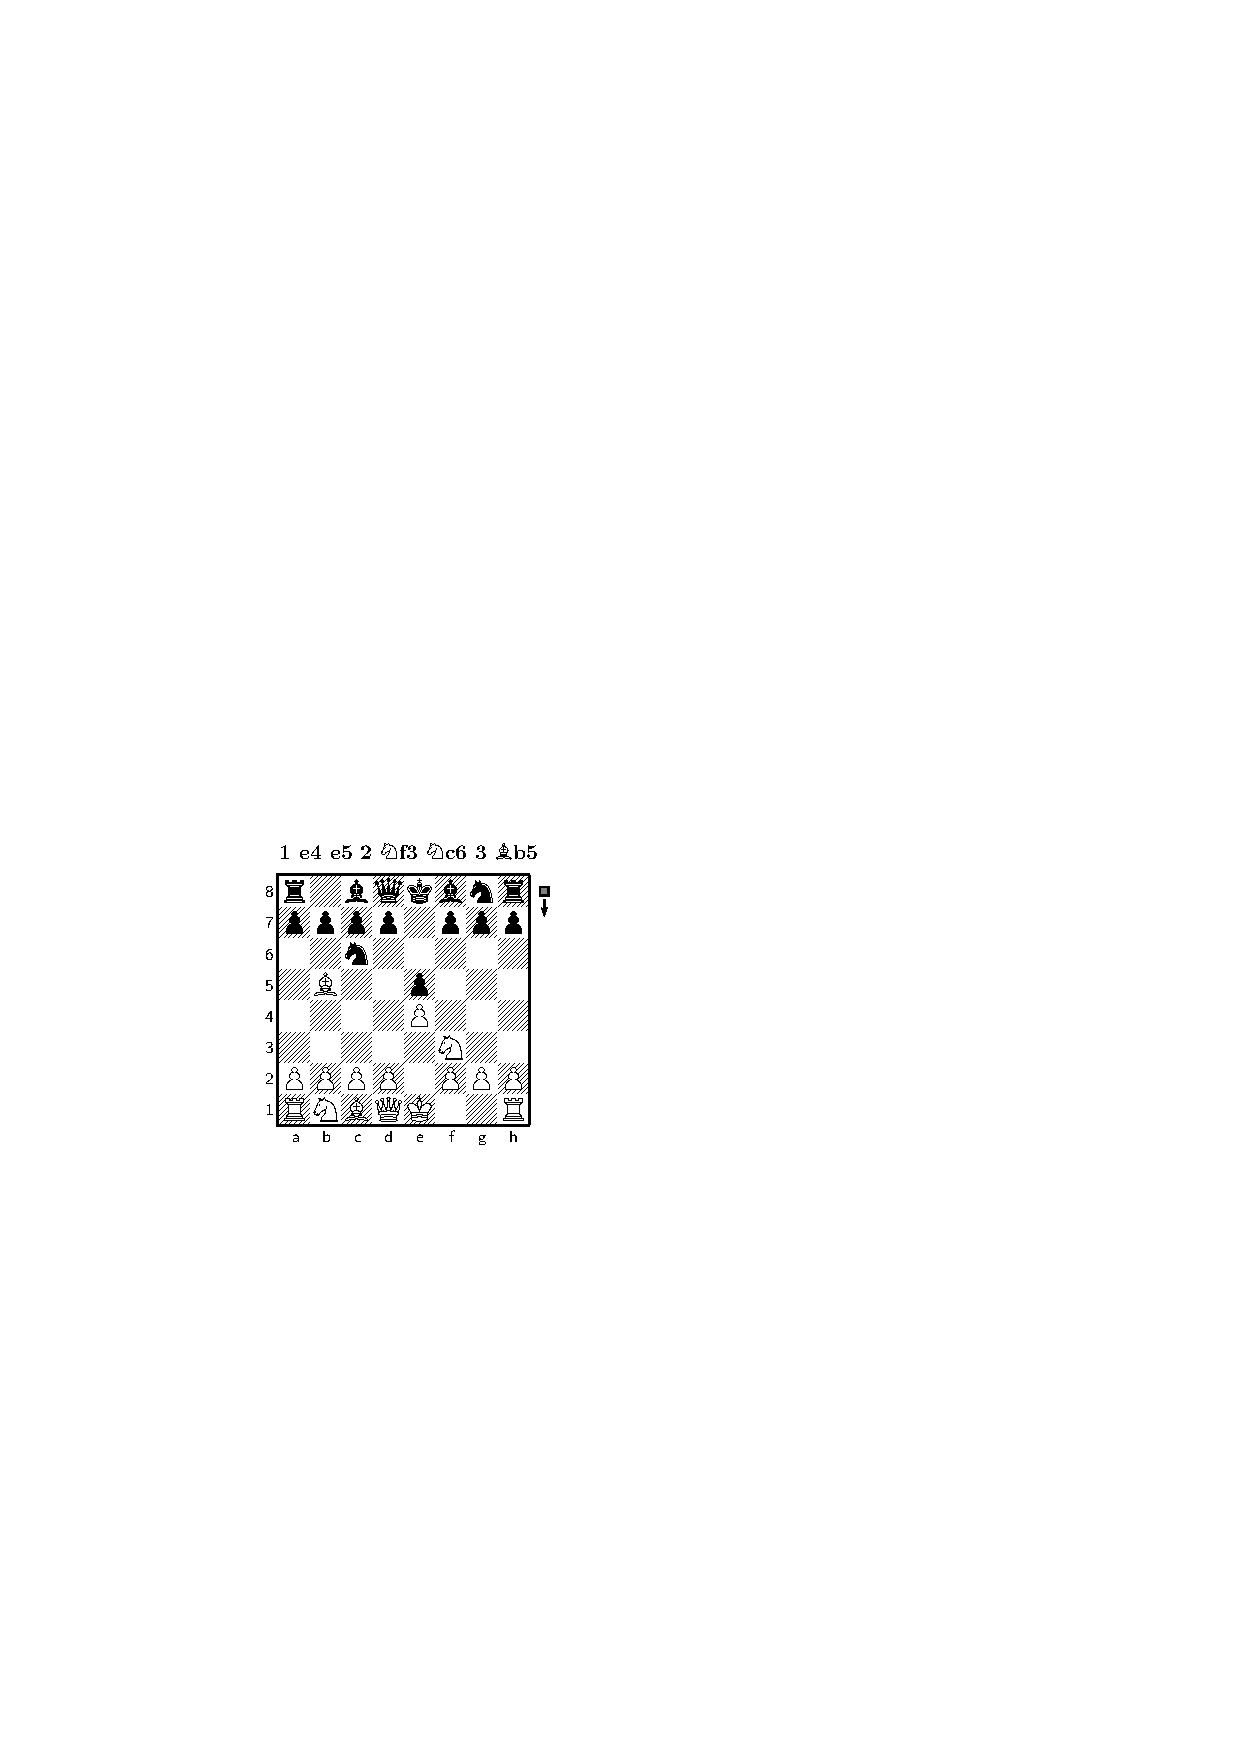
\includegraphics[width=\hsize]{tabuleiro}
    \end{LaTeXoutput}
  \end{column}
\end{columns}
\end{frame}

\begin{frame}{Produzindo partituras musicais com MusiX\TeX}
\begin{itemize}
\item MusiX\TeX{} é incluído no \TeX\ Live;
\item Leia a documentação com o comando \texttt{texdoc musixtex} 
\item Usa notação musical para descrever a partitura;
\item \LCmdArg{usepackage}{musixtex} e \LCmdArg{usepackage}{musixcpt}
\item Rosegarden (sequenciador de midi) -- \url{http://www.rosegardenmusic.com/}
\end{itemize}
\end{frame}

\begin{frame}{Um exemplo de partitura}\fontsize{11}{12}\selectfont
\begin{LaTeXcode}[Fonte da partitura]
\LCmdArg{begin}{music} \string\hsize=100mm \n
\LCmdArg{generalmeter}{\string\meterfrac24}\% \n 
\string\parindent 0pt \string\generalsignature{-3} \n 
\string\startpiece\string\bigaccid \string\NOtes\string\qu\Larg{ce}\string\en\string\bar \n
\string\NOtes\string\qu\Larg{gh}\string\en\string\bar \string\NOtes\string\qu\Larg{=b}\string\en  \n
\string\Notes\string\ds\string\cu g\string\en\string\bar \string\NOtes\string\qu\Larg{\string^f=f}\string\en\string\bar \n
\string\NOtes\string\qu\Larg{=e}\string\itied0e\string\qu\Larg{\string_e}\string\en\string\bar \n
\string\Notes\string\ttie0\string\Qqbu ed\Larg{\string_d}c\string\en\string\bar \n
\string\Notes\string\ibu0b\Larg{-2}\string\qb0\Larg{=b}\string\enotes \n
\string\notes\string\nbbu0\string\qb0\Larg{=a}\string\tqh0N\string\enotes \n
\string\Notes\string\Dqbu cf\string\en\string\bar \n
\string\NOtes\LCmdArg{uptext}{\string\it tr}\string\qu e\%\n
\LCmdArg{uptext}{\string\it tr}\string\qu d\string\en\string\bar \n
\string\NOtes\string\qu c\string\qp\string\en\string\Endpiece \n
\LCmdArg{end}{music} \n
\end{LaTeXcode}
\end{frame}

\begin{frame}{Um exemplo de partitura}
\begin{LaTeXoutput}\centering
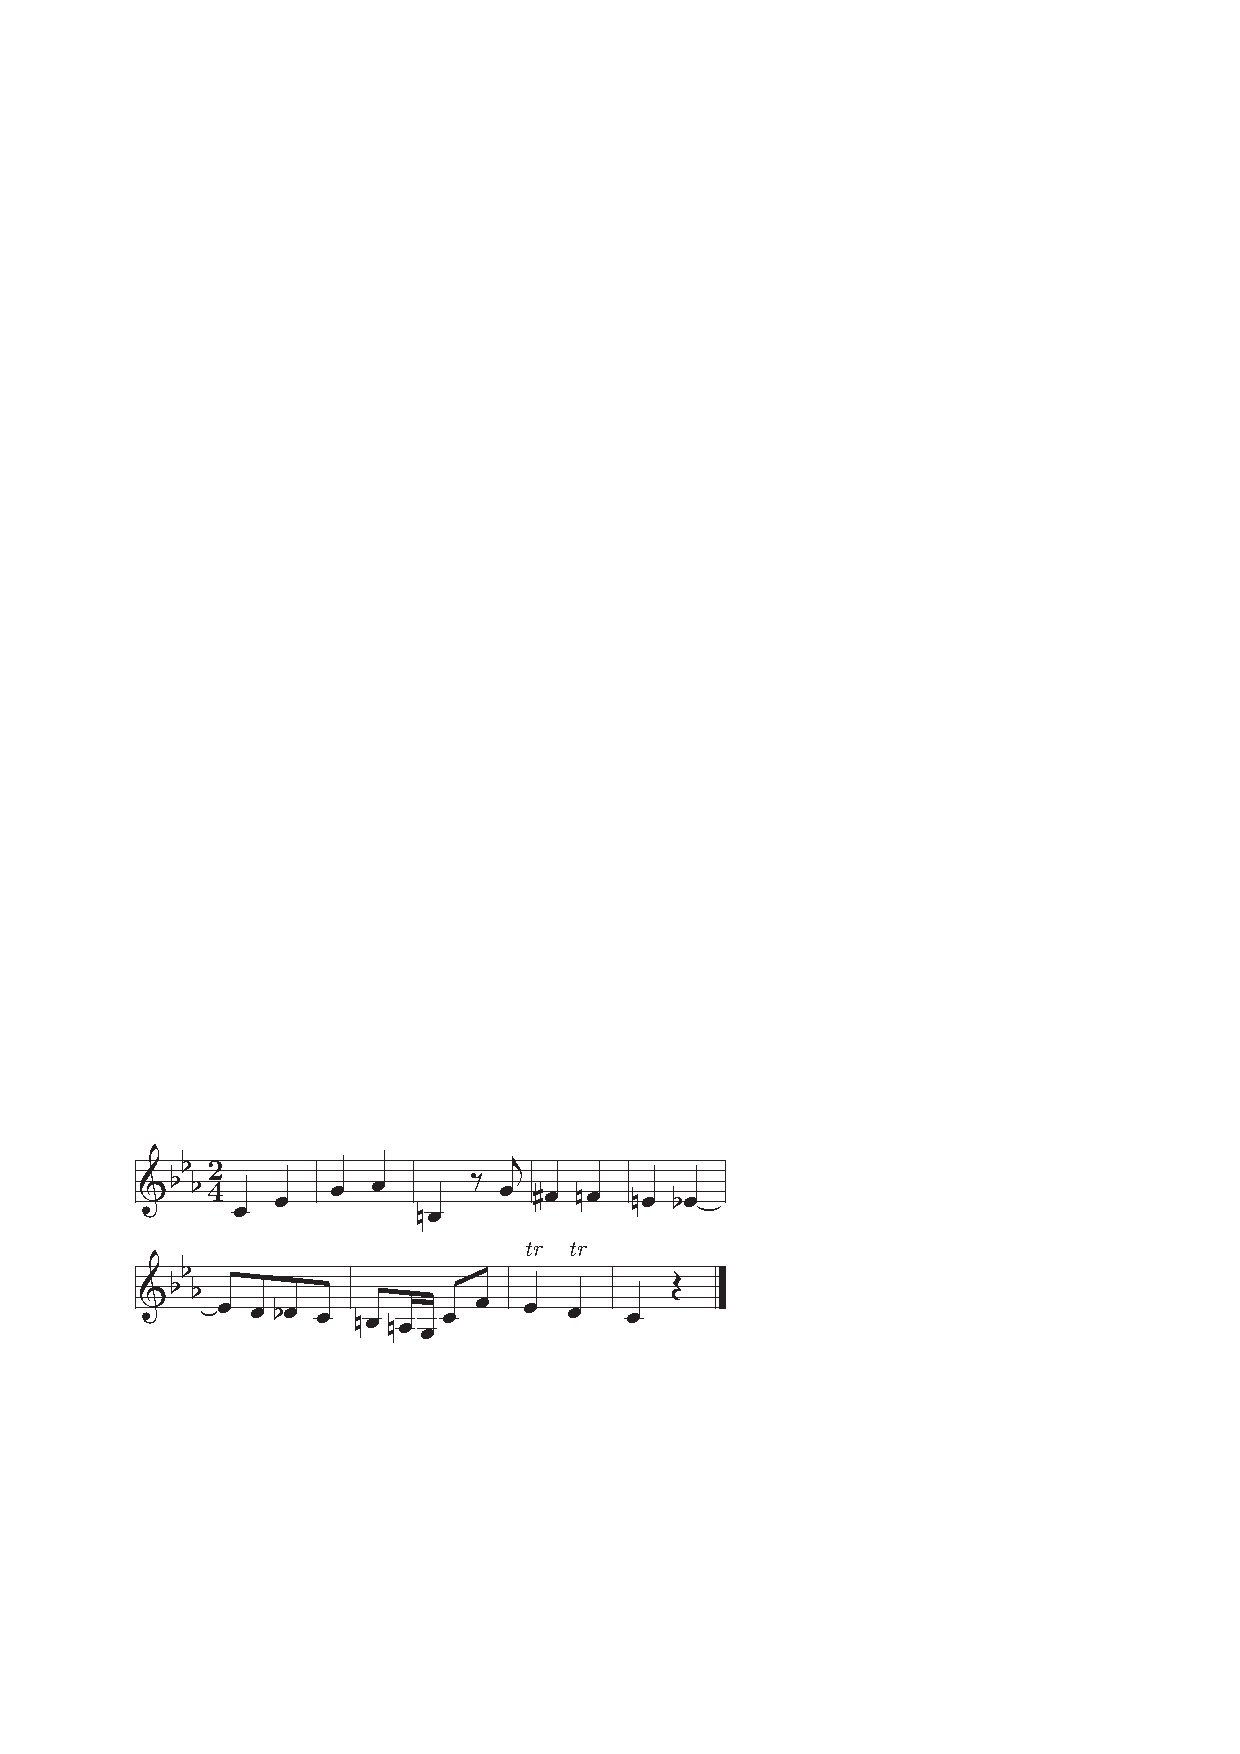
\includegraphics[width=\hsize]{Musica}
\end{LaTeXoutput}

\end{frame}

\begin{frame}[fragile]
\frametitle{Fórmulas químicas}
\begin{itemize}
\item \LaTeX\ possui pacotes para tipografia de textos científicos que, entre outras coisas, permitem a composição de fórmulas químicas;
\item Evita o excesso de subscritos típicos desse tipo de aplicação;
\item Leia a documentação com o comando \texttt{texdoc mhchem};
\item \LCmdOptArg{usepackage}{version=3}{mhchem}
\end{itemize}

\begin{LaTeXcode}[Exemplo]
\LCmdArg{ce}{C6H12O6}
\end{LaTeXcode}

\medskip

Produz:
\begin{LaTeXoutput}
\[ \mathrm{C}_6\mathrm{H}_{12}\mathrm{O}_6 \]
\end{LaTeXoutput}
\end{frame}




%\section{Aula 5}
%% Aula 5 - Beamer

\begin{frame}{Produzindo apresentações com Seminar}
\begin{itemize}
\item \Lsty{Seminar} é incluído no \TeX\ Live
\begin{LaTeXcode}[Declaração]
\LOA documentclass[slideonly,12pt]{seminar}
\end{LaTeXcode}
\item Para obter frame e sombreamento:
\begin{LaTeXcode}[Frame e sombreamento]
\LCmdArg{usepackage}{fancybox}\n
\LCmdArg{slideframe}{shadow}
\end{LaTeXcode}
\end{itemize}
\end{frame}

\begin{frame}{Seminar}

\begin{itemize}
\item Para definir um slide:
\begin{LaTeXcode}[Slide]
\LCmdArg{begin}{slide}\n
\dots\n
\LCmdArg{end}{slide}
\end{LaTeXcode}
\item Para continuar nos slides seguintes:
\begin{LaTeXcode}[Quebra de slide]
\LCmd{newslide}
\end{LaTeXcode}
\end{itemize}
\end{frame}

\begin{frame}{Beamer}
\begin{itemize}
\item Apresentações mais dinâmicas;
\item Incluído no \TeX\ Live;
\item Requer também os pacotes \Lsty{pgf} e \Lsty{xcolor};
\item Veja: \url{http://minerva.ufpel.edu.br/~campani/tutbeamer.tar.gz}
\item Uso:
\begin{itemize}
\item \LCmdArg{documentclass}{beamer};
\item Estrutura usando \LCmd{section} e \LCmd{subsection};
\item Slides individuais dentro de comandos \LCmd{frame};
\item Compilar direitamente com \prog{pdflatex}.
\item Veja: \url{http://www.tug.org/teTeX/tetex-texmfdist/doc/latex/beamer/beameruserguide.pdf}
\end{itemize}
\end{itemize}

\end{frame}

\begin{frame}{Exemplo de documento \LCmd[]{beamer} }
\fontsize{10}{11}\selectfont

\begin{LaTeXcode}[Exemplo]
\LCmdArg{documentclass}{beamer} \n
\LCmdArg{usepackage}{beamerthemesplit} \n
\LCmdArg{title}{Exemplo} \n
\LCmdArg{author}{Till Tantau} \n
\LCmdArg{begin}{document} \n
\LCmdArg{frame}{\LCmd{titlepage}} \n
\LOA section[Outline]{} \n
\LCmdArg{frame}{\LCmd{tableofcontents}} \n
\LCmdArg{section}{Introdução} \n
\LCmdArg{subsection}{Visão geral da classe Beamer} \n
\LCmdArg{begin}{frame}\Larg{Características da classe Beamer} \n
\null\quad  \LCmdArg{begin}{itemize} \n
\null\qquad  \LCmd{item}<1-> Classe \LCmd{LaTeX}\LCmd{ }normal. \n
\null\qquad  \LCmd{item}<2-> Fácil sobreposição. \n
\null\qquad  \LCmd{item}<3-> Sem necessidade de programas externos.  \n     
\null\quad  \LCmdArg{end}{itemize} \n
\LCmdArg{end}{frame} \n
\LCmdArg{end}{document} \n
\end{LaTeXcode}
\end{frame}

\begin{frame}{Alguns comandos de \LCmd[]{beamer}}
\begin{LaTeXcode}[Temas]
\LCmdArg{usetheme}{\dots}
\end{LaTeXcode}

\begin{LaTeXcode}[Frames]
\LCmdArg{begin}{frame}\Larg{Título do frame} \n
\dots \n
\LCmdArg{end}{frame} \nn
ou \nn
\LCmdArg{frame}{\LCmdArg{frametitle}{Título do frame} \n
\dots \n
}
\end{LaTeXcode}
\end{frame}

\begin{frame}{Alguns comandos de \LCmd[]{beamer}}
\begin{LaTeXcode}[Logo]
\LOA pgfdeclareimage[height=1.4cm]{logo}\Larg{unb}
\LCmdArg{logo}{\LCmdArg{pgfuseimage}{logo}}
\end{LaTeXcode}

\begin{block}{Observação}
arquivo de imagem: \texttt{unb.jpg} (retira-se a extensão)
\end{block}

\begin{LaTeXcode}[Blocos]
\LCmdArg{begin}{block}\Larg{Título do bloco} \n
\dots \n
\LCmdArg{end}{block}
\end{LaTeXcode}
\end{frame}

\begin{frame}{Colunas}
\begin{LaTeXcode}[Colunas]
\LCmdArg{begin}{columns}\LO[t]
 \nn
\LCmdArg{begin}{column}\Larg{5cm} \n
\dots \n
\LCmdArg{end}{column}
 \nn
\LCmdArg{begin}{column}\Larg{5cm} \n
\dots \n
\LCmdArg{end}{column}
 \nn
\LCmdArg{end}{columns}
\end{LaTeXcode}
\end{frame}

\begin{frame}{Overlays}
	\begin{LaTeXcode}[Overlays]
		\LCmdArg{begin}{itemize} \n
		\LCmd{item} <1-> Primeira coisa \n
		\LCmd{item} <2-> Segunda coisa \n
		\LCmd{item} <3-> Terceira coisa \n
		\LCmdArg{end}{itemize} \n
	\end{LaTeXcode}
	
	\begin{itemize}
	\item Especificação de overlay:
	\begin{itemize}
		\item \texttt{<3->} -- mostra do 3 em diante;
		\item \texttt{<2-5>} -- mostra entre o 2 e o 5;
		\item \texttt{<-4>} -- mostra até o 4.
	\end{itemize}
\end{itemize}
\end{frame}

\begin{frame}{Transparência}
Para obter transparência: 

\LCmdArg{setbeamercovered}{transparent}
  e usar  \LCmd{uncover} em substituição aos \LCmd{item}.
\end{frame}

\begin{frame}{Destacando}
\begin{LaTeXcode}[Destacando]
\LCmdArg{begin}{itemize} \n
\LCmd{item} <1- | alert@1> Primeira coisa \n
\LCmd{item} <2- | alert@2> Segunda coisa \n
\LCmd{item} <3- | alert@3> Terceira coisa \n
\LCmdArg{end}{itemize}
\end{LaTeXcode}
\end{frame}

\begin{frame}{Overlays com blocos}
\begin{LaTeXcode}[Overlays com blocos]
\LCmdArg{begin}{frame}\Larg{Overlays com blocos} \n
\LCmdArg{begin}{block}\Larg{Primeiro bloco}<1-> \n
Este é o primeiro bloco \n
\LCmdArg{end}{block}
\nn
\LCmdArg{begin}{block}\Larg{Segundo bloco}<2-> \n
Este é o segundo bloco \n
\LCmdArg{end}{block} \n
\LCmdArg{end}{frame}
\end{LaTeXcode}
\end{frame}

\begin{frame}{Efeitos nas transições de lâminas}

\begin{itemize}
\item \LCmd{transdissolve}
\item \LCmd{transsplitverticalout}
\item \LCmd{transblindshorizontal}
\item etc.
\end{itemize}
\end{frame}


\begin{frame}{Conclusão}
\begin{center}\color{red}
\fontsize{50}{60}\selectfont FIM
\end{center}
\end{frame}

\end{document}

